%\documentclass[english]{ipsj}
%\documentclass[english,preprint]{ipsj}
%\documentclass[english,preprint,JIP]{ipsj}
\documentclass[english,sigrecommended,JIP]{ipsj}

%\usepackage{graphicx}
%\usepackage[dvipdfmx]{graphicx}
\usepackage{latexsym}

\usepackage[hyphens]{url}
\usepackage{xpatch}

\def\Underline{\setbox0\hbox\bgroup\let\\\endUnderline}
\def\endUnderline{\vphantom{y}\egroup\smash{\underline{\box0}}\\}
\def\|{\verb|}

\usepackage{enumitem, kantlipsum}

\usepackage{tikz}
\usepackage{amsmath}
\usepackage{amssymb}

\usepackage{minipage}
\usepackage{ulem}
\usepackage{xcolor}
\usepackage{graphicx}
\usepackage{multirow}

\newcommand\reduline{\bgroup\color{red}\markoverwith{\textcolor{black}{\rule[-0.5ex]{2pt}{0.4pt}}}\ULon}
\newcommand\blueuline{\bgroup\color{blue}\markoverwith{\textcolor{black}{\rule[-0.5ex]{2pt}{0.4pt}}}\ULon}
\newcommand\violetuline{\bgroup\color{violet}\markoverwith{\textcolor{black}{\rule[-0.5ex]{2pt}{0.4pt}}}\ULon}
\newcommand\magentauline{\bgroup\color{magenta}\markoverwith{\textcolor{black}{\rule[-0.5ex]{2pt}{0.4pt}}}\ULon}
%\newcommand\magentauline{\bgroup\color{magenta}\markoverwith{\textcolor{black}{}}\ULon}
\newcommand\cyanuline{\bgroup\color{cyan}\markoverwith{\textcolor{black}{\rule[-0.5ex]{2pt}{0.4pt}}}\ULon}
\newcommand\orangeuline{\bgroup\color{orange}\markoverwith{\textcolor{black}{\rule[-0.5ex]{2pt}{0.4pt}}}\ULon}

\newcommand{\red}[1]{\textcolor{red}{#1}}
\newcommand{\blue}[1]{\textcolor{blue}{#1}}
\newcommand{\green}[1]{\textcolor{green}{#1}}

%\usepackage{extpfeil}

\renewcommand\UrlFont{\color{blue}\rmfamily}

\hyphenpenalty=10000\relax
\exhyphenpenalty=10000\relax
\sloppy

\setcounter{volume}{30}% vol25=2017
\setcounter{number}{1}%
\setcounter{page}{1}

%%\received{2020}{12}{31}
%\rereceived{2011}{10}{1}   % optional
%\rerereceived{2011}{10}{31} % optional
%%\accepted{2021}{12}{31}

\usepackage[varg]{txfonts}%%!!
\makeatletter%
\input{ot1txtt.fd}
\makeatother%

\begin{document}

%\title{MKM: Multiple Kernel Memory for Protecting Page Table Switching Mechanism Against Memory Corruption}
%\title{Design and Implementation of Kernel Memory Isolation for Container Resources}
% \title{Designing and Implementing of Kernel Memory Isolation Against Side-Channel Attack with Speculative Execution}

% \title{Mitigation of Side-Channel Attack with Speculative Execution Using Kernel Memory Isolation}
% \title{Mitigating Foreshadow Side-Channel Attack Using Dedicated Kernel Memory Mechanism}
% \title{vkTracer: Vulnerable Kernel Code Tracing to Generate The Profile of Kernel Vulnerability}
% \title{Identification of Vulnerable Kernel Code\\ Using Kernel Tracing Mechanism}
\title{KDPM: Kernel Data Protection Mechanism\\ Using a Memory Protection Key}



% \affiliate{kobe}{Department of Electrical and Electronic Engineering, Graduate School of Engineering, Kobe University, Hyogo, 657--8501, Japan}
\affiliate{kobe}{Graduate School of Engineering, Kobe University, Hyogo, 657--8501, Japan}
% \affiliate{okayama}{Graduate School of Natural Science and Technology, Okayama University, Okayama, 700--8530, Japan}
\affiliate{okayama}{Faculty of Natural Science and Technology, Okayama University, Okayama, 700--8530, Japan}


\author{Hiroki Kuzuno}{kobe}[kuzuno@port.kobe-u.ac.jp]
\author{Toshihiro Yamauchi}{okayama}[yamauchi@okayama-u.ac.jp]
% \author{Toshihiro Yamauchi}{okayama}[\violet{yamauchi@okayama-u.ac.jp}]

% # -*- coding: utf-8 -*-
\begin{abstract}
  % オペレーティングシステムカーネルへの攻撃として,カーネル脆弱性を利用したメモ
  % リ破壊によるカーネルデータの改ざんが知られており,特権昇格攻撃やセキュリティ
  % 機能の無効化が可能とされている.
  % オペレーティングシステムカーネルへの攻撃として,カーネル脆弱性を利用
  % して権限情報を管理者権限に改ざんする特権奪取攻撃が知られている.
  % A known attack on operating system kernels is the modification of kernel data
  The kernel data of an operating system kernel can be modified
%  faces the modification of kernel data 
  through memory corruption by exploiting kernel vulnerabilities. 
  %
  % It achieves that 
  Memory corruption allows privilege escalation and defeats security mechanisms.
  %
  % メモリ破壊により,
  % %
  % カーネルへの攻撃困難化として, KCoFIでは,カーネルコードの呼出し順序の検査を行
  % い,カーネルコードの実行順序の保証, KASLRによるカーネルコード,およびカーネル
  % データの仮想アドレス配置のランダム化がある.また,AKOでは,特権奪取を行う際の
  % 権限情報の変化に着目し,意図しないタイミングでの権限情報の変化検知を行い,書き
  % 戻す事を可能とした.
  % To make it difficult to attack the kernel, 
  % KCoFI 
  The kernel control flow integrity verifies and guarantees the order of
  invoking kernel codes.
  %invocations to guarantee the sequence of kernel code execution, 
  The kernel address space layout randomization randomizes the virtual address
  layout of the kernel code and data. 
  %
  % In addition, 
  The additional kernel observer focuses on the unintended privilege
  modifications to restore the original privileges.
  % , when performing privilege
  % revocation, the focusing on changes in authorization information, the system
  % detects changes in authorization information at unintended times and writes
  % them back to the The new system enables the user to restore the original
  % settings.
  % %
  % KASLRはカーネルコード,およびカーネルデータの仮想アド
  % レスのランダム化を行うことで攻撃困難化を実現する.
  % カーネルにおける攻撃対策として,KCoFIでは,カーネルコードの呼出し順序
  % の検査を行い,KASLRはカーネルコード,およびカーネルデータの仮想アド
  % レスのランダム化を行うことで攻撃困難化を実現する.
  % %
  % また,AKOでは,特権奪取を行う際の権限情報の変化に着目し,意図しない
  % タイミングでの権限情報の変化検知を行い,書き戻す事を可能とした.
  % %
  % しかし,これら既存手法のセキュリティ機構では,カーネルデータへの書込みは禁止
  % されない.攻撃を行うユーザプロセスによる権限情報の書込み制限は行わないことか
  % ら,依然としてカーネル脆弱性の利用に成功した場合,権限情報の改ざんは可能であ
  % る.
  % カーネル脆弱性の利用に成功した場合,カーネルデータは依然として改ざん可能であ
  % り,特権昇格やセキュリティ機能が無効化される可能性は存在する.
  % However, these existing security mechanisms do not prohibit writing to kernel
  % data. It is still possible to overwrite
  However, these existing security mechanisms do not prevent writing to the
  kernel data. Therefore, kernel data can be overwritten by exploiting kernel
  vulnerabilities. Additionally, privilege escalation and the defeat of security
  mechanisms are possible.
  %

  % Vulnerable kernel codes are a threat to an operating system kernel. An
  % adversary's user process can forcefully invoke a vulnerable kernel
  % code to cause kernel memory corruption or denial of service (DoS) on
  % a running kernel.
  % %
  % Attack mitigation strategies, including prevention and isolation
  % mechanisms require modifying kernel design and performance cost.
  % %
  % Moreover, approaches to reduce the vulnerability of kernel codes, such as
  % kRazor and KASR, analyze entire applications and kernel behavior to generate
  % the necessary kernel code for each application.
  % %
  % However, these approaches do not determine the kernel codes even if they are
  % invoked at the exploitation of the kernel. Moreover, the running kernel still
  % contains the vulnerable kernel codes, which are the main threat.
  % %
  % In addition, the detail of vulnerable kernel codes is not provided from the
  % common vulnerabilities and exposures (CVE).
  % %
  %
  % 我々はカーネルにおいて特定のカーネルデータを保護するセキュリティ機構を提案し
  % ており,Memory Protection Key (MPK)を利用し,カーネルデータへの書込み制限
  % 制御を可能としている.    
  %
  % 本稿では,既存手法の課題を解決するため,特定のカーネルデータへの書込みを制限
  % し,権限情報の保護に利用可能なセキュリティ機構を提案する.
  %
  % 提案するセキュリティ機構では,Memory Protection Key を利用し,カーネルデータ
  % の仮想アドレスに対する書込み制限の制御を行う.
  %
  % 提案したセキュリティ機構では,ユーザプロセスの権限情報の保護機能,セキュリ
  % ティ機能に関するカーネルコードの保護機能を提供する.提案しているセキュリティ
  % 機構の拡張性を検討し,書き込み制限対象領域の細粒度化と負荷低減のための機能に
  % ついて考察を進めた.
  %
  % In this paper, 
  %We propose a novel security mechanism that restricts the writing of specific
  We propose a kernel data protection mechanism (KDPM), which is a novel
  security design that restricts the writing of specific kernel data. 
  %
  This mechanism protects privileged information and the security mechanism to
  overcome the limitations of existing approaches.
  %  the security inadequacy of existing approaches.
  %in order to solve the problems of existing approaches.
  %
  The KDPM adopts a memory protection key (MPK) to control the write
  restriction of kernel data. 
  %
  % The proposed security mechanism provides protection capability for user
  % process authorization information and kernel code related to security
  % functions. 
  %  
  % the proposed security mechanism dynamically restricts writing
  %
  The KDPM with the MPK ensures that the writing of privileged information for user
  processes is dynamically restricted during the invocation of specific system
  calls. 
  % the dynamic restriction of the writing of privileged information of user processes 
  %
  %In addition, 
  To prevent the security mechanisms from being defeated, the KDPM dynamically
  restricts the writing of kernel data related to the mandatory access control
  during the execution of specific kernel codes.
  %
  % The extensibility of the proposed security mechanism was examined, and the
  % granularity of the write-restricted area and functions to reduce the load were
  % discussed.
  % %
  % % 攻撃を行うユーザプロセスによる,特権奪取時の権限情報の改ざんを防ぐため,実行
  % % 中のカーネルにおいて,ユーザプロセスに対して,動的に権限情報の書込み制限を実
  % % 現.ならびに,セキュリティ機能の無効化を防ぐため,カーネルに対して動的に強制
  % % アクセス制御に関するカーネルデータの書込み制限を実現する.
  % %
  % In order to prevent user processes from falsifying privilege information
  % during privilege seizure, the kernel dynamically restricts writing of
  % privilege information to user processes during execution. In addition, to
  % prevent the disabling of security functions, the kernel dynamically restricts
  % the writing of kernel data related to mandatory access control to the kernel.
  % %
  % 攻撃を行うユーザプロセスによる,特権奪取時の権限情報の改ざんを防ぐため,実行
  % 中のカーネルにおいて,動的にカーネルデータの書込み制限を実現する.本稿では,
  % 既存手法の課題を解決するため,特定のカーネルデータへの書込みを制限し,権限情
  % 報の保護に利用可能なセキュリティ機構を提案する.
  % %  
  % 提案するセキュリティ機構では,Memory Protection Key を利用し,カーネルデータ
  % の仮想アドレスに対する書込み制限の制御を行う.
  % %
    %
  % To address the threat of kernel vulnerabilities, this study proposes a
  % vulnerable kernel code tracing mechanism (vkTracer), which employs an
  % alternative viewpoint using a proof-of-concept (PoC) code that contains the
  % starting points of a kernel attack process.
  % %
  % vkTracer analyzes the user process of the PoC code to hook the invocation of
  % the vulnerable kernel codes on the running kernel. 
  % %
  % It employs the kernel tracing features (i.e., \verb|kprobe| and
  % \verb|tractpoints|) to attach the kernel while the user process invokes
  % vulnerable kernel codes.
  % %
  % Moreover, vkTracer extracts the whole kernel component's information using
  % running and static kernel image and debug section.
  % %
  % It ensures that vkTracer identifies the virtual address range and function
  % name of the invoked kernel code; then, it creates a profile of kernel
  % vulnerability.
  % %
  % Therefore, the kernel attack surface is reduced, or the kernel is isolated
  % from the effect of vulnerable kernel codes (i.e., CVE registered kernel
  % vulnerability) using the profile generated by vkTracer without kernel
  % reconfiguration.
  % %
  % %
  % 提案方式は,MPKを利用可能なエミュレータ上の Linux にて実現しており, Linuxに
  % て実現している.評価のため特権奪取に利用可能なカーネル脆弱性を導入した環境に
  % おいて,攻撃を行うユーザプロセスによる権限情報の書込み防止可能性について評価
  % した.
  Further, the KDPM is implemented on the latest Linux with an MPK emulator. 
  % For the purpose of evaluation, 
  We also evaluated the possibility of preventing the writing of privileged
  information. 
  % by the attacking user process through a kernel vulnerability that can
  % achieve privilege escalation. in an environment where a kernel vulnerability
  % that can be used to steal privileges has been introduced.
  %
  % 権限情報保護機能の性能評価として,システムコール呼出しに対して 2.96\% から
  % 9.01\% のオーバヘッドであること,ならびにMPK操作にかかる性能負荷を計測した.
  The KDPM showed an acceptable performance cost, measured by the overhead, which 
  was from 2.96\% to 9.01\% of system call invocations, whereas the performance load
  on the MPK operations was 22.1 ns to 1347.9 ns.
  %
  Additionally, the KDPM requires 137 to 176 instructions for the
  implementations.
  %
  % The evaluation results indicated that vkTracer could trace PoC code
  % executions (e.g., kernel memory corruption and DoS), identify vulnerable
  % kernel codes, and generate kernel vulnerability profiles.
  % %
  % Furthermore, the implementation of vkTracer revealed that the
  % identification overhead ranged from 5.2683 s to 5.2728 s on the PoC
  % codes,
  % %
  % the maximum system call latency was 3.7197 $\mu$s, and the acceptable overhead
  % of 100,000 Hypertext Transfer Protocol sessions via the web client program
  % ranged from 0.37 \% to 0.56 \%. 
\end{abstract}

%reducing the vulnerable of a kernel code include
  %These approaches show that it is difficult to avoid only the vulnerable kernel
  %Existing approaches to reducing the vulnerable of a kernel code include
  %kRazor and KASR, which analyze applications and kernel behavior to
  %generate necessary kernel code for each application.
  %kRazor and KASR analyze applications and kernel behavior for the
  %generation of necessary kernel code for each application for
  %kernel attack surface reduction.
  %vkTracer dynamically analyzes the user process of the PoC code to

  %
  %However, for stability, it is necessary to trace the entire kernel
  %code invocation for kernel attack surface reduction;
  %% vkTracer dynamically analyzes the user process of PoC
  %% code to hook the invocation of vulnerable kernel code on the
  %% running kernel.  Moreover, vkTracer identifies the virtual address
  %% range and function name of the invoked kernel code using kernel
  %% debug information; then it creates a profile of kernel vulnerability.
  %
  %
   %approaches for kernel attack surface reduction can

  %Therefore, the approaches of kernel attack surface reduction can
  %exclude only vulnerable kernel code using vkTracer's profile.
    %an adversary's user process can not execute 
    %}  
  %employ the reference of unmapped kernel page to on the running kernel.
  %
  %\reduline{  
  %applications,
  %% The evaluation results demonstrated vkTracer successfully
  %% generate the profiles of kernel vulnerability that were introduced
  %% from PoC code attacks (e.g., kernel memory corruption and DoS).
    %that may lead to 
    %}
    %\reduline{
  %In addition, the implementations of vkTracer indicated
  %the tracing overhead latency
    %

    %
    %Moreover, vkTracer represents 2.459 \% and 2.193 \% as the dynamic
    %kernel tracing overhead.
      %the web client program  access
    %%   overhead of 100,000 Hypertext Transfer Protocol sessions.
    %}
  %and prevents actual
  %that 
  %
  %% \reduline{
  %%   %In addition, the performance results of the KPRM indicated limited
  %%   %kernel processing overhead in benchmarks and a low impact on user
  %%   %applications.
  %%   In addition, the implementations of KPRM indicates that the
  %%   maximum system call overhead latency is 0.703 $\mu$s, while the
  %%   the web client program was from 1.188 \% to 4.093 \% access
  %%   overhead of 100,000 Hypertext Transfer Protocol sessions.
  %%   %
  %%   Moreover, the implementations of KPRM attained 2.459 \% and 2.193
  %%   \% as the kernel compiling time overhead.  }

%%   software benchmarks and a low impact on user
%% applications.
  
%%   low kernel processing overhead in 

%%   can protect the
%%   kernel code and kernel data from a proof-of-concept kernel
%%   vulnerability that could
%%   %
%%   In addition, the performance results of the MKM indicated
%%   low kernel processing overhead in benchmarks and user applications.  

%% %
%% We implemented KPRM on the latest Linux kernel
%% %
%% and showed that it successfully thwarts actual proof-of-concept kernel
%% vulnerability attacks that may cause kernel memory corruption.
%% %
%% In addition, the KPRM performance results indicated limited kernel
%% processing overhead in software benchmarks and a low impact on user
%% applications.

%% \begin{keywords}
%%   Kernel vulnerability, Dynamic analysis, System security, Operating system
%% \end{keywords}

% \begin{IEEEkeywords}
%   Kernel vulnerability, Dynamic analysis, System security, Operating system
% \end{IEEEkeywords}

  %}
    %that %is small program and
    %the invocation placement of vulnerable kernel code within 
    %that relies on 
    %}  
    %the vulnerable kernel
    %code list as a profile, then accept profile to dynamically unmaps
    %the kernel page of vulnerable kernel code. This also protects
    %attack target kernel data.
  %% \blueuline{[N-01]
  %% An adversary's user process compromises the operating system (OS)
  %% kernel. The vulnerable kernel code leads kernel memory corruption.
  %% %
  %% It could overwrite the kernel data containing privilege information
  %% of user process or the kernel code related to security features
  %% (i.e., mandatory access control).
  %% %
  %% %The operating system (OS) comprises a mechanism for sharing the kernel
  %% %address space with each user process.
  %% %
  %% Operating systems researcheres have proposed kernel protection
  %% methods.
  %% %
  %% The approachees of multiple kernel address space divide one kernel
  %% address space to protect kernel memory from memory corruption (e.g.,
  %% Process-local memory and system call isolation).
  %% %
  %% %While user processes create their own kernel address space,
  %% These methods have still kept the vulnerable kernel code on the
  %% kernel memory.
  %% }
  %% %
  %オペレーティングシステムへの攻撃として,カーネル脆弱性を
  %利用したメモリ破壊による特権奪取や競合条件の発生による動作停止が指摘
  %されている.
  %
    %\reduline{
    %OS researcheres have proposed kernel attack surface reduction
    %that provides the minimizing of visible kernel code to mitigate
    %the invocation of vulnerable kernel code from the user process
    %(e.g., kRazor and KASR).
    %
  %These methods
  %Existing approaches for kernel attack surface reduction include
  %Further, these need to trace the entirety of the invocation kernel
  %codes for the stability; it is difficult to only avoid the
  %vulnerable kernel code that is main threat in the kernel memory.
    %that is still located in the kernel memory.
    %when the application and kernel update.
    %latest kernel vulnerability is disclosed, it 
    %}
  %
  %This is because the discovered vulnerable kernel code 
  %
  %% \blueuline{  
  %% To comprises a kernel, adversaries focus on the invocation of latest
  %% vulnerable kernel code that relies on the starting points of the
  %% kernel attack process.
  %% %
  %% An adversary's user process can involve malicious code that elevates
  %% from user mode to kernel mode.
  %% %
  %% Herein, to prevent such subversion attacks, we present the kernel
  %% page reducing mechanism (KPRM), which employs an alternative
  %% design and approaches for novel kernel attack surface reduction.
  %% %
  %% The objective of KPRM mechanism focuses on the prohibition of
  %% vulnerable kernel code execution and prevents writing to the kernel
  %% data from an adversary's user process.
  %% }
  
  %
  %This removes
  %The KPRM manages the reference of the unmapped kernel page from the kernel
  %page table at the system call invocation.
  %
    %Additionally, the KPRM achieves that identification and unmapping of
    %vulnerable kernel code to prevent exploit the kernel through latest
    %kernel vulnerability.
  %
    %\reduline{


\maketitle

\footnotetext{This paper is an extended version of a paper published
  in the 23rd World Conference on Information Security Applications (WISA 2022) \cite{kuzuno22wisa}.}

% # -*- coding: utf-8 -*-
\section{Introduction}\label{seciton:introduction}
% オペレーティングシステム(OS)カーネルに対する攻撃として,特権昇格攻撃とセキュ
% リティ機能の無効化攻撃が課題とされている.
%
The operating system (OS) kernel encounters threats, in which privileges may be
escalated and security mechanisms may be defeated.
% defeat of security mechanism.
% attacks are considered 
% %
% これらの攻撃は,攻撃者のユーザプロセスが,脆弱性を含むカーネルコード(以降,
% カーネル脆弱性)を利用し,メモリ破壊を起こし,権限情報の改ざん,ならびにセキュ
% リティ機能の回避のためにセキュリティ機能に関するカーネルデータを改ざんする攻撃
% である.
% These attacks are attacks in which 
The user process of the adversary exploits the kernel code containing
vulnerabilities (i.e., vulnerable kernel code), thereby corrupting the memory.
%resulting in memory corruption.
%
The kernel vulnerability is reported by the Common Vulnerabilities and Exposures
(CVE). The CVE has the Common Platform Enumeration that indicates the naming of
systems, software, and packages.
%
Until August 2022, xx CVE with CPE of Linux and CVE description contains kernel
memory vulnerabilities were issued in the CVE of National Vulnerability Databse
(NVD)\cite{nvd}, as shown in \figref{fig:linux_memory_cve}.

% It achieves the illegal modification of privileged information and alters kernel
% data of the security mechanism to take full administrator privileges.
%
Therefore, privileged information can be modified and kernel data of the security
mechanism can be altered to gain full administrator privileges.
%  bypass security functions.
% %
% 攻撃事例として,特権奪取攻撃に加え,セキュリティ機能の無効化攻撃ではアクセス
% 制御特権昇格攻撃に加え,セキュリティ機能の無効化攻撃の事例では,
%
% 攻撃事例として,アクセス制御に関するカーネルデータを改ざんの後,管理者権限に昇
% 格し,制限の回避が試みられる\cite{nexus5exploit,grsecurity}.
% From and actual attack case, 
The actual kernel memory corruption cases indicate that the modifying the kernel data
related to mandatory access control (MAC), the user acquires administrator
privileges and circumvents the MAC restrictions \cite{nexus5exploit,grsecurity}.

% オペレーティングシステム(OS)カーネルへの攻撃として,権限情報を管理者
% に改ざんする特権奪取攻撃が課題とされている.
% 特権奪取攻撃は,攻撃を行うユーザプロセスが脆弱性を含むカーネルコード
% (以降,カーネル脆弱性)を利用し,カーネル仮想記憶空間上に配置され,権
% 限情報を格納したカーネルデータに対し,一般ユーザから管理者ユーザ
% に改ざんする攻撃である.
% %
% 攻撃を行うユーザプロセスは計算機の管理者ユーザとして,マルウェアの実行
% や隠蔽を行い,他の計算機への攻撃を試みる.

%
% An operating system (OS) kernel must have the ability to tackle
% vulnerable kernel codes, which can otherwise lead to memory corruption
% or denial of service (DoS), among other problems.
% %
% Moreover, such attacks can leverage privilege escalation or service
% disruption to cause further damage, or suspend the running kernel altogether
% \cite{chen11linux}.

% カーネル脆弱性を介した攻撃の防止手法として,Kernel Address Space Layout
% Randomization (KASLR)は,カーネルコードやカーネルデータの仮想アドレスをランダ
% ム化し,攻撃時の仮想アドレスの特定を困難化した \cite{shacham04ccs}.
% %
% また,不正コード呼出し制限のため,KCoFIでは,コード呼出し順を検査するControl
% Flow Integrity(CFI)\cite{abadi05ccs}をカーネルに適用可能とした
% \cite{criswell14sp}.

% カーネル脆弱性を利用した攻撃の防止手法として,KCoFIでは,コード呼出し
% 順を検査する control flow integrity(CFI)\cite{abadi05ccs}をカーネル
% に適用可能とし,不正なコード呼出しを制限した \cite{criswell14sp}.
% As a method to prevent attacks using kernel vulnerabilities, KCoFI enables
The following are the countermeasures that can prevent kernel attacks via
vulnerable kernel code. Kernel control flow integrity (KCoFI)
% enables control flow integrity (CFI) 
inspects the order of code execution \cite{abadi05ccs} to restrict the
kernel code from being illegally invoked \cite{criswell14sp}.
% Kernel address space layout randomization (KASLR)では,カーネルの仮
% 想記憶空間上のカーネルコードやカーネルデータの仮想アドレスをランダム化
% し,攻撃時の仮想アドレスの特定を困難化した \cite{shacham04ccs}.
Kernel address space layout randomization (KASLR) randomizes the virtual
addresses of the kernel code and kernel data in the kernel memory space to foil
attacks \cite{shacham04ccs}, whereas
% This makes it difficult to identify the virtual address during an attack
%
% また,特権奪取攻撃対策として,Additional kernel observer(AKO)は,カーネルに
% おける権限情報変化に対し,意図しない書替えを検知した場合,元の権限情報に修正
% し,特権奪取攻撃の防止を実現している \cite{yamauchi21ijis}.
%In addition, 
the additional kernel observer (AKO) detects unintentional rewriting in response
to the changes in the privileged information of user processes against a privilege
escalation attack \cite{yamauchi21ijis}.
% the original privilege information
% when it This prevents privilege-grabbing attacks
% \cite{yamauchi21ijis}.

% 既存の手法により,カーネルにおける,カーネル脆弱性を介したカーネルデータ改ざん,
% ならびに不正コード呼出しは軽減される.しかし,攻撃が成功した場合,権限情報やセ
% キュリティ機能に関するカーネルデータは改ざん可能であり,以下の課題があると考えて
% いる.
% 既存の手法では,ユーザプロセスからの特権奪取攻撃の成立困難化として,脆
% 弱なカーネルコード特定,呼出し,ならびに被害の抑制を行う.しかし,権限
% 情報に対する攻撃自体は可能であり,次の課題があると考えている.
% Existing techniques 
%These mitigate illegal modifications of kernel data via kernel vulnerabilities.
These mitigate the kernel data from being illegally modified via kernel
vulnerabilities.
% and malicious code calls in the kernel. 
However, if the kernel memory is successfully corrupted, kernel data can be
overwritten.
%authorization information and security functions 
%
%
% Kernel hardening approaches adopt software and hardware based
% mechanisms. Kernel control flow integrity \cite{abadi05ccs}, kernel
% address randomization (KASLR) \cite{shacham04ccs}, and kernel isolation
% \cite{proclocal,sci} are mechanisms used to harden kernel codes and data
% against attacks.
% %
% A central processing unit (CPU) privilege mechanism provides access and
% execution restrictions between the user and the kernel mode \cite{smap-smep}.
% %
% However, the running kernel still contains vulnerable kernel codes,
% which can be invoked from an adversary's user process.
% \begin{enumerate}[topsep=0pt, leftmargin=1.2cm]%\itemsep=-1.0ex \parskip=1.0ex
%   \item [課題]: {\bf メモリ破壊によるカーネルデータの改ざん}\\
%     %
%     動作中のカーネルは,カーネルモードにおいて,カーネルデータの書込み制限は行わない.カーネル脆弱性
%     を利用し,メモリ破壊に成功する場合,攻撃者は権限情報やセキュリティ機能に関する
%     カーネルデータを書替え可能である.
%     %
%     従来手法では,セキュリティ機能に関するカーネルデータの書込み制限の制御は行われ
%     ないことから,改ざん防止は困難である.
% 特権奪取攻撃では,権限情報の改ざんとして,一般ユーザから管理者ユーザ
% へのユーザIDの書替えが行われる.
% %
% 従来手法では,権限情報は動作中のカーネルに対して読書き制限の制御は行
% われない.
% %カーネルモードにおいては読書き権限の制御は行われていない.
% %
% 実行されたカーネルコードには権限情報の書替え制限は行われないことから,
% 攻撃を行うユーザプロセスから脆弱なカーネルコードを実行された場合,権
% 限情報の改ざんを防ぐことは難しい.
% We consider the following issue induces 
We consider that a running kernel does not restrict the writing of kernel data
in the kernel mode. 
% If the kernel vulnerability is exploited and memory corruption succeeds,
% an adversary can rewrite kernel data. 
% related to authorization information and security functions.
%
Existing approaches do not control the write restrictions of kernel data related to
privileged information and security mechanisms. Therefore, an adversary can 
gain full administrator privileges.
% still take 
% , making it difficult to preventtampering.
%
%     %
% \end{enumerate}
% The identification and restraint of vulnerable kernel code in a running
% kernel is challenging. 
% %
% Although the common vulnerabilities and exposures (CVE) summarizes the overviews
% of kernel vulnerability, these report does not contain the detail of vulnerable
% kernel codes.
% %
% As modern kernels are complex and lengthy, it is hard to identify which kernel
% codes relate to which kernel vulnerabilities.
% %
% In addition, the removal of kernel codes can affect the stability of a user
% process or kernel.

% %
% Approaches, such as KASR and kRazor can reduce the kernel attack surface
% of a running kernel by restraining the vulnerable kernel code \cite{kurmus14dimva,
% zhang18arxiv}.
% %
% These approaches trace benign applications, related kernel codes, and kernel data to
% statically create available kernel images. It is necessary to regularly
% update the software to account for all applications and kernel-related behavior.
% %
% However, the past approaches do not target proof-of-concept (PoC) codes, which are
% small malicious program codes that target the invocation of vulnerable kernel codes
% to attack the kernel.

% 本稿では,特権奪取攻撃における,権限情報の改ざんを緩和するため,特定のカーネル
% データを保護対象(以降,保護対象カーネルデータ)として,書込み制限を動的に制御
% するセキュリティ機構を提案する.
In this study, we propose a kernel data protection mechanism (KDPM), which is
a novel security capability that dynamically controls the write restrictions of
specific kernel data as protected kernel data. 
% (hereinafter referred to as "protected kernel data").
% %
% \figref{fig:approach_overview}に提案手法の概要を示す.提案するセキュリティ機構
% では攻撃の種別に応じ,実現方式1,および実現方式2を備える.実現方式1では,汎用
% 性を重視し,特権昇格攻撃を防止する権限情報保護機能を実現している.実現方式1で
% は,ユーザプロセスに対し,予め許可されたシステムコール発行時のみに保護対象カー
% ネルデータへの書込みを許可する.
Figure \ref{fig:approach_overview} provides an overview of the KDPM,
%  is shown in Figure
%
% The proposed security mechanism 
which determines whether system calls and kernel codes have write permission of
the kernel data in the kernel layer.
%
To ensure kernel data protection and managing write restrictions, the KDPM
adopts the Intel memory protection key (MPK), which is a protection keys for
supervisor (PKS).
%
A PKS provides a protection key that handles write restrictions for each page of
kernel data.
% is specified for the kernel

%When a vulnerable kernel code is executed by the user process of an adversary,
%
The KDPM assumes that the user process of an adversary invokes a vulnerable
kernel code which attempts to modify the kernel data related to privileged
information or security mechanism.
%
The KDPM focuses the mitigation of the illegal overwritten of these kernel
data.
%as protected kernel data.}
% through the kernel memory corruption vulnerability. 
%
The privileged information is changed by specific system calls and the policy of
MAC is modified by specific kernel codes. Moreover, the function pointers of the MAC
are never modified at the running kernel.
%
%\cyanuline{ 
The KDPM provides a straightforward application of the PKS to maintain simple
design of the kernel data protection. Additionally, the KDPM combines the
characteristics of system calls, kernel code behavior, and hardware features. 
%}
%
The limitation of the KDPM is a little difficult to support frequently modified kernel data. 


\begin{figure}[tb]
  \centering        
  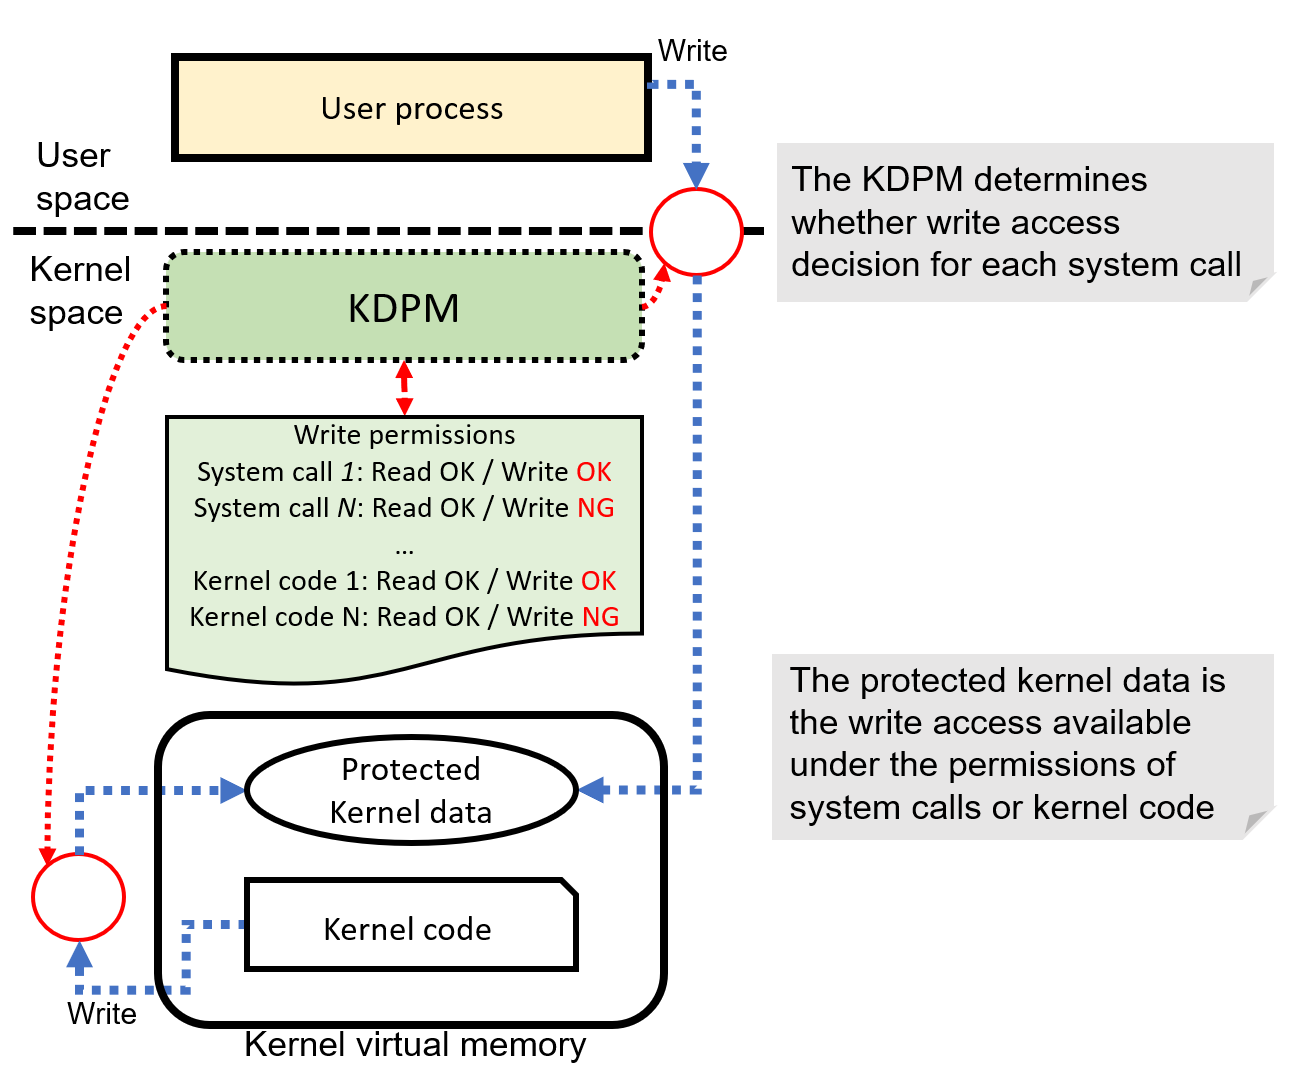
\includegraphics[bb=0 0 972 809, scale=.240]{./imgs/001_screenshot_2021-07-26_17.18.08.png}
  % \vspace{-2.0ex}  
  \caption{
    %
    %提案するセキュリティ機構の概要
    Overview of the kernel data protection mechanism
    %
  }
  \label{fig:approach_overview}
  %\vspace{-5.0ex}
  % \vspace{-2.0ex}  
\end{figure}


% Because the kernel allows the changing of privileged information using specific
% system calls. Additionally, the kernel has never modified the function pointer
% of MAC, and rarely changes MAC policy using specific kernel codes.}
% the privileged information or kernel data of security mechanism 

% the kernel memory corruption vulnerability
% that leads illegal overwritten of these kernel data. 
% that requires the memory write operation
% will not succeed unless the kernel disables the write restriction based on the
% PKS protection key.
% \red{The KDPM prevents the illegal overwritten of these kernel data through the
% kernel memory corruption vulnerability that requires the memory write operation
% will not succeed unless the kernel disables the write restriction based on the
% PKS protection key.}

The KDPM has two implementations that focus on the different types of kernel
attacks.
% i 1 and Realization 2, depending on the type of attack.
%
Implementation 1 is a general purpose for the protection of privileged
information to prevent privilege escalation. This allows user processes to write
to protected kernel data only when write-permitted system calls are invoked.
%
% 実現方式2として,カーネルデータの書き込み制限対象領域の細粒度化とオーバヘッド
% 低減を可能とする,セキュリティ機能の無効化攻撃を防止のためのセキュリティ機能保
% 護機能を検討する.実現方式1では,カーネルに対し,予め許可されたカーネルデータ
% の実行時のみに保護対象カーネルデータへの書込みを許可する.
Implementation 2 protects the kernel data of the security mechanism (e.g., MAC)
%protection function
to prevent security mechanism from being defeated. This reduces overheads to
limit the write restriction timing of protected kernel data.
%granularity and
Further, Implementation 2 allows the protected kernel data to be written only
when executing a write-permitted kernel code.

\begin{itemize}[topsep=0pt]%\topsep=-1.0ex \itemsep=-1.0ex \parskip=1.0ex
%   \item {\bf 実現方式1}:特権昇格攻撃の防止のため,ユーザプロセスの権限情報の保護を目
%   的とし,システムコール単位にて権限情報の書込み制限を制御する手法
%   \item {\bf 実現方式2}:セキュリティ機能の無効化攻撃の防止のため,カーネルコード単位
%   にてセキュリティ機能に関するカーネルデータの書込み制限を制御する手法  


\item {\bf Implementation 1}: To prevent a privilege escalation attack,
Implementation 1 controls the write restriction of privileged information in each
write-permitted system call to protect the privileged information of user processes.
% for the purpose of protecting privilege information of user processes.

\item {\bf Implementation 2}: 
% on security functions, a method to 
Implementation 2 controls the write restriction of the kernel data related to
the security mechanism in each write-permitted kernel code to prevent the
defeating security mechanism attack.


\end{itemize}

% 両実現方式においては,保護対象カーネルデータに対してPKS の Protection keyを指
% 定し書込み制限を行う.攻撃を行うユーザプロセスにより,脆弱なカーネルコードを実
% 行された場合,権限情報やセキュリティ機能に関するカーネルデータの改ざんが試みら
% れるが,権限情報Protection keyに基づく書込み制限をカーネルが無効にしない限り,
% 書込みは成功しない.
% data to be protected, and  
% an attempt is made to tamper with

%
Intel CPUs containing a PKS are not available as of March 2022 and will be implemented
on the next generation CPUs; however, a PKS is available in the QEMU environment
\cite{qemu}.
%
This study is an early application of the forthcoming PKS to protect kernel
data.
%
The following are the contributions of this study:
%
% 脆弱なカーネルコードが呼ばれた場合において
% も,権限情報とセキュリティ機能に関するカーネルデータの不正な改ざんを保護でき,
% 特権昇格攻撃,ならびにセキュリティ機能の無効化攻撃の緩和に繋がる.
%
% 

%
% 権限変更を伴わないシステムコールを介し,攻撃を行ユーザプロセスから権限情報の改ざんの困難化を実現する.
% また,セキュリティ機能
% に関するカーネルデータを保護対象とした場合,セキュリティ機能と関連しないカーネ
% ルコードを介し,攻撃を行うユーザプロセスから権限情報の改ざんの困難化を実現す
% る.

% 提案するセキュリティ機構により,保護対象カーネルデータに対して,PKSを
% 利用した読書き制限の制御が可能になる.
% %
% 権限情報に対して PKS の Protection key (以降,権限情報 Protection
%   key)を指定し,保護対象とすることで,脆弱なカーネルコードが呼ばれた
% 場合においても,権限情報を保護でき,特権奪取攻撃の緩和に繋がる.
% %
% %実現方式においては,
% 提案するセキュリティ機構では,権限情報 Protection key による書込み制限
% をシステムコール発行時に制御し,予め許可されたシステムコール発行時のみ,
% 権限情報の書替えを許可する.
% %
% これにより,攻撃を行うユーザプロセスにおいて,脆弱なカーネルコードを実
% 行された場合,特権奪取攻撃による権限情報の改ざんが試みられるが,権限情
% 報Protection keyに基づく書込み制限をカーネルが無効にしない限り,権限情
% 報への書込みは成功しない.


% セキュリティ機構においては,Intel Memory Protection Key (MPK)Protection Keys
% for Supervisor(PKS)\cite{intel-mpk,pks}を用いて,カーネルデータへの書込み制
% 限を行う.
% %
% PKSはカーネルモードに対し,メモリへの読書き可否を制御する Intel CPUの機能であ
% る.2022年1月時点ではハードウェアは提供されておらず,QEMU環境でのみPKSを利用で
% きる \cite{qemu}.

% 我々は, 動作中のカーネルにおいて,特定のカーネルデータを保護するためのセキュリ
% ティ機構を提案しており\cite{kzn21css},\figref{fig:approach_overview}に概要を示
% す.先行提案の



% This leads to the following research problem that addresses how we can easily
% identify the vulnerable kernel codes and then provide the restraining kernel
% code a list of kernel vulnerabilities,
% %
% so that the removal/isolation of these kernel codes can be performed smoothly
% for a running kernel. 
% %
% It requires the detail of vulnerable kernel codes contains function names or
% virtual addresses of kernel codes leads the kernel exploitation.
%

% 提案するセキュリティ機構においては,保護対象カーネルデータへの書込み制
% 限を Intel Memory Protection Key (MPK)Protection Keys for Supervisor
% (PKS)を用いて制御する.
% %
% PKSは,Intelにより開発中のMPKの機能であり,現在のMPKはユーザモードに対
% するメモリ読書き可否を制御できる.
% %
% PKSはスーパーバイザモード(本稿ではカーネルモードとする)に対し,
% %
% %PKSは,カーネルモード実行中に
% メモリへの読書き可否を制御する機能であり,Persistent memory での利用が
% 検討されている \cite{pks, pks-pmem}.MPK はページテーブルエントリ(PTE)
% 毎に Protection key を指定し,読書き制限の設定を可能とするCPU機能であ
% る(詳細は\ref{seciton:background_mpk}節を参照).
% %
% PKSをサポートするIntelプロセッサは2021年8月時点では提供されておらず,
% 次世代CPUへ実装予定であるが\cite{intel-mpk-cpu},QEMU環境ではPKSを利用
% 可能である\cite{qemu}.
% %
% PKSをカーネルのセキュリティ機構として利用する提案はまだなく,
% %
% 本研究では今後登場するPKSをカーネルの重要なデータの保護に逸早く適用
% するものである.



% This paper describes the features of a novel security approach known
% as the vulnerable kernel code tracing mechanism (vkTracer).
% %
% It has a tracking mechanism that identifies the information of vulnerable kernel
% codes that contains virtual address ranges and kernel function names
% to create a restricted kernel code list, which serves as the profile of kernel
% vulnerabilities.
% %adversary’s 
% %
% It focuses on the behavior of an actual PoC code,
% which subverts the running kernel.


% 提案するセキュリティ機構により,保護対象カーネルデータに対して,PKSを
% 利用した読書き制限の制御が可能になる.
% %
% 権限情報に対して PKS の Protection key (以降,権限情報 Protection
%   key)を指定し,保護対象とすることで,脆弱なカーネルコードが呼ばれた
% 場合においても,権限情報を保護でき,特権奪取攻撃の緩和に繋がる.
% %
% %実現方式においては,
% 提案するセキュリティ機構では,権限情報 Protection key による書込み制限
% をシステムコール発行時に制御し,予め許可されたシステムコール発行時のみ,
% 権限情報の書替えを許可する.
% %
% これにより,攻撃を行うユーザプロセスにおいて,脆弱なカーネルコードを実
% 行された場合,特権奪取攻撃による権限情報の改ざんが試みられるが,権限情
% 報Protection keyに基づく書込み制限をカーネルが無効にしない限り,権限情
% 報への書込みは成功しない.



% vkTracer achieves the following objectives:
% %%
% To identify the vulnerable kernel code, vkTracer executes a PoC code
% that is available online as a user process and then uses kernel tracking
% to record the entire kernel code invocation.
% %
% Next, it extracts the virtual address ranges and function names
% of the vulnerable kernel code as the profile.
% %
% vkTracer manually exploits known kernel vulnerabilities (e.g., CVE).
% %
% It ensures that the profile contains information about the identified
% vulnerable kernel code that relates to memory corruption or DoS.

% The implementation of vkTracer reserves the attaching placement of kernel code
% invocation using the kernel tracing features (i.e., \verb|kprobe| and
% \verb|tractpoints|) while the execution of PoC code.
% %
% Moreover, vkTracer prepares the kernel component information for the profile
% generation. It can relate the virtual address range and function name of kernel
% codes to invocated kernel codes using running and static kernel image contains
% debug with an attributed record format (DWARF) and symbol information.
% %
% It ensures that vkTracer identifies the invoked kernel code, and then
% creates a profile of kernel vulnerability.

% %
% The vkTracer profile can facilitate kernel attack surface reduction or
% kernel isolation approaches. vkTracer can generate the profile of the latest
% vulnerable kernel code to restrict or separate a running kernel when the
% latest PoC code is disclosed with a kernel vulnerability.

% 本稿では,2つの実現方式の機能検討と考察を行い,MPK PKS 利用時における性能評価に
% ついて検証を行なった:


% This study's primary contributions are as follows: %of this study are summarized as follows:
% We studied and discussed the functionality of the two realizations, and verified
% the performance evaluation when using MPK PKS. 

%\vspace{-1.0ex}

\begin{enumerate}[topsep=0pt]%\itemsep=-1.0ex \parskip=1.0ex
%   \item
% カーネル脆弱性を利用した特権奪取攻撃,およびセキュリティ機能無効化の緩和のため,
% 動作中のカーネルにおけるカーネルデータ保護を備えるセキュリティ機構を提案し,設計した.
% %
% 提案手法においては, PKS を利用し,実現方式1として,システムコール発行時の権限情
% 報への書込み制限,および,実現方式2として,カーネルコード実行中におけるセキュリ
% ティ機構に関するカーネルデータの保護を実現した. 
%\item We designed a novel security mechanism that protects kernel data in the
\item We designed the KDPM that protects the kernel data in the running kernel to
prevent privilege escalation and defeat of security mechanism attacks through
vulnerable kernel code.
% vulnerabilities and disabling security features.
%
% In the proposed method, 
The implementations of the latest Linux kernel use a PKS to handle the write restriction
of the kernel code during a specific system call or specific kernel code execution.
% is information, and as implementation method 2,
% The kernel data concerning the security mechanism is protected.

% 管理するセキュリティ機構を提案した.
%実現方式1および2の処理の共通化,ならび
%     に保護対象とするカーネルデータの違いに起因する制御タイミングを比較した.
% 
% め,PKS を利用し,システムコール発行時,およびカーネルコード実行中における
% 権限情報への書込み制限を
% 管理するセキュリティ機構を提案した.
% %
% 動作中のカーネルを対象として,提案手法を実現した Linux にて,セキュリティ機能
% を検証した.


  \item 
% 提案するセキュリティ機構の評価として,特権奪取攻撃に利用可能なカーネル脆弱性を
% カーネルに導入し,攻撃を行うユーザプロセスによる権限情報の改ざんを防止可能である
% ことを確認した.提案するセキュリティ機構の実現方式1におけるシステムコール呼出し
% にかかるオーバヘッドは  2.96\% から 9.01\% であること,ならびにMPK PKS の書込み
% に 22.1 ns,レジスタ操作の読込みに 30.5 ns,および書込みに1347.9 ns の処理負荷が
% かかることを示した.
% As an evaluation of the KDPM,
To evaluate the KDPM,
%we introduced a kernel vulnerability occurs privilege escalation and 
we confirmed that the kernel with Implementation 1 can prevent the modification of privileged
information by the adversary's user process. Additionally, we confirmed that the kernel
with Implementation 2 can prevent the defeat of security mechanisms.
%
The overhead of Implementation 1 requires latency of system call ranging from
2.96\% to 9.01\%, 
% the system call call in the proposed security mechanism
and the processing time for the kernel with Implementation 2 for writing the PKS
is 22.1 ns. Furthermore, reading the register operation requires 30.5 ns, and
writing the register operation requires 1347.9 ns.
% The results are shown below.

% \item 提案するセキュリティ機構の評価として,特権奪取攻撃に利用可能なカー
%   ネル脆弱性をカーネルに導入し,攻撃を行うユーザプロセスによる権限情報
%   の改ざんを防止可能であることを確認した.
%   また,通常アプリケーションおよびカーネルへの影響可能性を検討した.

\end{enumerate}
  
% \begin{enumerate}

% \item The proposed vkTracer method is a novel approach for tracking
%   the vulnerable kernel code for an adversary's user process at the
%   kernel layer.
%   %
%   The key functionality of vkTracer is  to identify
%   vulnerable kernel code information (e.g., virtual address ranges and
%   function names) on the modern OS kernel.
%   %
%   This paper presents the tracing model, security features, limitations,
%   portability of vkTracer, and any future research directions envisioned.

  
% \item The effectiveness of the vkTracer implementation is based on how well
%   it identifies the invocation of vulnerable kernel codes through
%   proven kernel vulnerabilities using the PoC code.
%   %
%   The measurement of the implementations of vkTracer reveals that 
%   the tracing overhead is between 5.2683 s and 5.2728 s for user applications,
%   %
%   the maximum round time overhead for system call is 3.7197 $\mu$s,
%   and the access overhead for 100,000 Hypertext Transfer Protocol (HTTP)
%   downloads via a web application is between 0.37 \% and 0.56 \%.


% \end{enumerate}
% 

%% The operating system (OS) kernel must tackle with vulnerable kernel
%% codes that can cause memory corruption or Denial of Service (DoS).
%% %
%% It can leverage privilege escalation or suspend the running kernel \cite{chen11linux}.
%kernel vulnerability
%  
%The operating system (OS) thwarts 
% to compromise computer devices.
%
%% \blueuline{
%%   The vulnerable kernel code that relys on the user processes share
%%   the kernel address space in the kernel mode; then an adversary's
%%   user process can execute vulnerable kernel code to
%%   overwrite kernel code and kernel data in
%%   %through kernel vulnerability attacks in
%% } \cite{kemerlis14usenix}.
%  can execute 
%  rely on
%hen,


%% \blueuline{
%%   To prevent kernel memory corruption,
%%   researchers proposed that
%%   the kernel protection mechanism provides security capabilities
%%   for each attack method.
%% }
%% \blueuline{
%% In} \cite{abadi05ccs}, \blueuline{the authors have proposed that
%% the kernel adopts a verification of kernel control flow integrity (CFI).
%% %
%% The kernel uses kernel address randomization (KASLR)
%% for the hardening of kernel code and kernel data identification in}
%% \cite{shacham04ccs}.
%% %
%% \blueuline{
%% Moreover, a CPU privilege mechanism provides he supervisor mode access
%% prevention (SMAP) forcefully denies access, and the supervisor mode
%% execution prevention (SMEP) prevents execution between the user mode
%% and the kernel mode in} \cite{smap-smep}.
%% %on the user region.
%% %
%% \blueuline{
%% In} \cite{proclocal}, \blueuline{the authors demonstrated 
%% process-local memory (Proclocal) allocates a specific
%% kernel address space for a user process.}
%% %
%% \blueuline{The authors in} \cite{sci} \blueuline{designed system call
%%   isolation (SCI) creates a dedicated kernel address space for the
%%   processing system call's routines.}
%
%%  kRazor  manages  the approval list of kernel code invocation to user
%% process has been proposed
% however these are not completely solve vulnerable kernel 
% the automatic vulnerable kernel code identification is important
% bud difficult to trace and identify the which kernel code is vulnerable 
% because kernel code cannot harml itself when poc invoke these code 
% take a damge to the kernel behavior
% reducing approache mitigate the potentially remove vulnerable kenrel code
% however not to identify actual vulnerable kenrel code
% these approache require entire kernel and app behavior
% to use it combine the isolation or hrdening approaches to cover the kernel 
% resilience? 
% By restraining vulnerable kernel code, approaches for reducing the
% kernel attack surface enhance security assurance for a running
% kernel.
% %
% For example, kRazor manages a privilege list, which controls whether a
% benign application has permission to call the kernel code \cite{kurmus14dimva}.
% %
% %On the other hand
% However, kernel attack surface reduction (KASR) provides a
% kernel image handling mechanism that controls the visible kernel code
% and kernel data of a virtual machine from the hypervisor, also for
% benign applications \cite{zhang18arxiv}.
%
%% To restrain vulnerable kernel code, the reducing of the kernel attack
%% surface approaches enhance security assurance for the running kernel.
%% %
%% kRazor can manage the privilege list which controls whether
%% the benign application has permission to call the kernel code 
%% %
%% Kernel attack surface reducing (KASR) provides a kernel image handling
%% mechanism that controls the visible kernel code and kernel data of
%% virtual machine from the hypervisor for benign application
%% \cite{zhang18arxiv}.
%
%
%
%These countermeasures can effectively mitigate the invocation of
%These approachees mitigate the invocation of vulnerable kernel codes. 
%However, these approaches leave some of problems unsolved.
% kRazor and KASR 
%It requires the tracing of benign applications, related kernel code, and kernel
%These countermeasures can effectively mitigate the invocation of
%vulnerable kernel code, thereby leave problem unsolved.
  %}
%While these approaches can 
%corruption, they leave two issues remain unaddressed.
%
%% \blueuline{ First, the running kernel still requires full kernel page
%%   mapping of kernel code and kernel data.}
%% %
%% \blueuline{
%% Second, Proclocal and SCI can protect kernel data of specific kernel
%% components without user process-related information owing
%% to stable behavior for kernel processing.}
%% %and SCI creates a statically duplicated kernel address space for each user process 
%
  %\reduline{
%% kRazor and KASR require the tracing of benign application, , related
%% kernel code, and kernel data to statically create the available kernel
%% code list or statically kernel image.
%%   %
%% This is necessary to update the software to account for all
%% application and kernel related behavior.
%
%}
%
%\blueuline{Nevertheless, these assure that potentially vulnerable kernel code and
  %attack targeted kernel code or remaining kernel data share the same
%  attack targeted kernel data share the same kernel address space.}
%
%% \reduline{The invocation of latest vulnerable kernel code at the kernel
%%   layer remains an unaddressed threat.}
%% %
%% \blueuline{ In} \cite{nexus5exploit,grsecurity}, \blueuline{the
%%   authors have already demonstrated that the latest attack idea can
%%   invoke the vulnerable kernel code to escalate privileges and evade
%%   security features (i.e., mandatory access control (MAC)) of SELinux
%% in} \cite{selinux}) \blueuline{for the running kernel.}
%% This paper describes the features of a novel security approach known
%% as the vulnerable kernel code tracing mechanism (vkTracer).
%% %}
%% %  which is a security capability enhancement that identifies vulnerable kernel codes.}
%% %
%% %\reduline{
%% It has the tracking mechanism that can identify vulnerable kernel code
%% information that contains virtual address ranges and kernel function
%% names to create the restriction kernel code list as the adversary's
%% profile.  It focuses on the behavior of actual Proof-of-Concept (PoC)
%% code that subverts the running kernel.
  %}
%
%% \blueuline{Additionally, KPRM has the restriction mechanism that can extend the controlling
%%   of vulnerable kernel code invocation and kernel data access of an
%%   adversary's user process on the running kernel.  }
%%   %  
%%   KPRM uses two types of kernel pages, namely, normal kernel pages and
%%   restricted kernel pages, to run the kernel and user processes.
 %
  %
%% \reduline{KPRM adopts the adversary's profile to assign
  %%   vulnerable kernel code and protected kernel data (e.g., user
  %%   identifiers) to a restricted kernel page; }
  %KPRM assigns vulnerable kernel code and protected kernel data (e.g.,
  %% \blueuline{
  %%   then, KPRM stores the remaining kernel code and kernel data in normal kernel pages.
  %% }
  
    %
%vkTracer achieves the objectives.
%such that vulnerable kernel code is 
%can dynamically 
%vkTracer ensures that the kernel can dynamically reduce the kernel
%attack surface, such that vulnerable kernel code is restricted to the
%running kernel.

%% %  }
%% vkTracer can manually exploit the already known kernel vulnerability
%% (e.g., common vulnerabilities and exposures (CVE)).
%% %
%% To identify the vulnerable kernel code, vkTracer dynamically executes
%% the PoC code online available as user process, then uses the kernel
%% tracking that records the whole of kernel code invocation. Then It
%% extracts the virtual address ranges and function names of vulnerable
%% kernel code as the adversary's profile.
%% %
%% vkTracer ensures that kernel can dynamically reduce the kernel attack
%% surface where vulnerable kernel code is restricted on the running
%% kernel.
    %}
  %% \blueuline{
  %%   Second, KPRM manages the assurance of kernel page handling
  %%   that the adversary's user process can not access restricted
  %%   kernel page references in their own kernel address space to mitigate
  %%   memory corruption.
  %% %
  %%   Finally, KPRM dynamically unmaps restricted kernel page references
  %%   of vulnerable kernel code using the adversary's profile
  %%   for the adversary's user process at the system call invocation.
  %%   }
  %

  %% KPRM applies this mechanism to all user processes without benign
  %% identification, \blueuline{which is manually registered to the benign user process
  %% list on the running kernel.
  %
  %the kernel address space is shared by both vulnerable kernel
  %code and attack target kernel data.
  %kernel address spacecode and attack target kernel code or kernel data.


  %
  %% \blueuline{
  %%   The implementation of KPRM provide two types of attack surface reducing
  %%   prototypes on the latest Linux kernel.
  %% }
  %% %
  %% \reduline{
  %%   This consideration corresponds that the user of KPRM adjusts
  %%   the protection of kernel code and kernel data owing the 
  %%   kernel address space processing performance cost for the running kernel.
  %%   }
  %% %
  %% \blueuline{
  %%   The first implementation provides an additional kernel address space
  %%   to enhance a security capability. It reserves vulnerable
  %%   kernel code of the adversary's profile and protected kernel data
  %%   kernel address spacefor restricted kernel pages
  %%   to prohibit the invocation of vulnerable kernel code and
  %%   the access of kernel data for the adversary's user process.
  %% }
  %% %
  %% \blueuline{The additional kernel address page
  %%   is managed as the dedicated kernel page table.
  %%   %
  %%   KPRM prepares process-context identifiers (PCID) of the translation
  %%   lookaside buffer (TLB) for each page table.
  %%   It reduces the TLB flushing cost
  %%   when the kernel executes the switching of kernel address spaces.
  %%   }
  %% %
  %% \blueuline{
  %%   The second implementation aims to lower the overhead. It is possible
  %%   to reserve protected kernel data of the adversary's profile for
  %%   kernel address spacerestricted kernel pages owing
  %%   to user processes sharing kernel address space.
  %%   }
  %% %
  %% KPRM only handles kernel page references of kernel code related to
  %% \blueuline{the profile of adversary's user process and the protected
  %%   kernel data} for reducing kernel misuse during interruption
  %% processing.

%In short, the primary contributions of this study are summarized as follows:
%The
    %% The proposed vkTracer, is a novel approach of
    %% tracking of vulnerable kernel code for an adversary's user
    %% process at the kernel layer.

    %% %
    %% The key requirements of vkTracer identified vulnerable kernel code
    %% information (e.g., virtual address ranges and function names) on
    %% modern OS kernel.
    %% %
    %% This paper also discusses the tracing model, security features,
    %% limitations, portability, and future work of vkTracer.
    %% %kernel attack surface   reducing to mitigate kernel memory corruption.}

    %access overhead.

    %% The effectiveness of vkTracer implementations is based on how well
    %% they identify the invocation of vulnerable kernel code
    %% through proven kernel vulnerabilities of PoC code.
  %
    %
    %Moreover, vkTracer indicates system benchmarks overhead of 2.459
    %\% to 2.193 \% for Linux kernel dynamic tracing.
 %   }
  %
  %% \blueuline{
  %%   The measurement of KPRM's performance using software benchmarks and 
  %%   applications such as the Apache web server and compiler.
  %%   %
  %%   %The evaluation results indicate that KPRM implementations have
  %%   %low latency overhead effects for the kernel and acceptable cost for
  %%   %user application processing.
  %%   KPRM performance evaluation results indicate that the maximum round time
  %%   overhead for system call is 0.703 $\mu$s.
  %%   %
  %%   The overhead for 100,000 Hypertext Transfer Protocol (HTTP) download
  %%   via a web application from 1.188 \% to 4.093 \% access overhead.
  %%   %
  %%   Moreover, the implementations of KPRM achieved an acceptable performance score that
  %%   indicates the kernel compiling time overhead of 2.459 \% and 2.193 \% for Linux kernel.
  %% }
% through kenrel vulnerabilities}.  
% kernel isolation and hardening are mitigation and prevention
%containted at the running kernel; then the vulnerable kenrel code 
% a running kernel. 
%Because many kernel codes are contained
%in the modern kernels. It 
% to enhance security assurance for 
%is not tracing target for  
%subvert the running kernel.}
% list or a static kernel image. 
%It can smoothly support 
% common vulnerabilities and exposures (CVE)).


% # -*- coding: utf-8 -*-
\section{Background} \label{seciton:background}

\subsection{Memory Protection Key}
% MPK は仮想アドレスを構成するPTEに対して読書き権限を操作可能な Intel
% CPU の機能である.\figref{fig:mpk_overview}に示す通り,PKS はカーネル
% モード用の MPK であり,次の機能が提供される\cite{intel-mpk}.
% MPK is an Intel CPU feature that allows manipulation of read permissions for
% PTEs that comprise a virtual address. As shown in \figref{fig:mpk_overview}, PKS
% is the MPK for kernel mode and provides the following functions
% \cite{intel-mpk}.

% \item Protection keys for supervisor(PKS):カーネルモードで利用する
%   Protection keyである.Control register 0(CR0)Write Protect フラグ
%   かつ CR4 PKS フラグにて有効 / 無効を制御する.
%   %
%   PKS では,PTEに対し,4 bit 割当てられ,16 個の Protection key を指定可能である.
%  Protection key 毎の読書き制限(Write
%     disable(WD),Read disable(RD))2 bit 操作のため, 32bitの読書き
%   制限操作レジスタIA32\_PKRS MSRレジスタ(以降,PKRS)をCPUコア毎に備える.

% MPK は Intel CPU の提供するセキュリティ機能であり,仮想記憶空間のペー
% ジ単位(Page Table Entry, PTE)にて読書き制限を制御可能とする \cite{intel-mpk}.
% %
% MPK では,ユーザモードで利用する Protection Keys for Userspace(PKU)と
% 読書き制限操作レジスタ Protection Key Right for User-mode (PKRU),
% ならびにカーネルモードで利用する Protection Keys for Supervisor(PKS)と
% 読書き制限操作レジスタ \verb|IA32_PKRS_MSR| レジスタ(以降,PKRS)がある.

Intel CPU provides an MPK, which is a security feature provided to control read
and write restrictions on a page basis, that is, page table entry (PTE)
\cite{intel-mpk}.
% in virtual memory space 
%
The MPK includes protection keys for userspace (PKU) and the protection key
right for user mode register for the user mode.
% the There are 
In addition, the MPK includes PKS and \verb|IA32_PKRS_MSR| register
(hereinafter, PKRS) for the kernel mode.

%the PTE has a 4-bit protection key (Pkey) for 16 Pkeys, 
As shown in Figure \ref{fig:mpk_overview}, the PTE has 16 4-bit protection keys
(Pkeys), and the 32-bit flag (two bits per Pkey: write disable (WD) and access
disable (AD)) controls the read and write restriction for each Pkey 
% basis via 
% In addition, read restriction is

The read and write restriction for Pkey {\it i} ($0 \leq i \leq 15$) is performed via the
register. If the value of bit AD {\it i} $\times$ 2 is 0, read is allowed. In contrast,
if the value of bit AD {\it i} $\times$ 2 is 1, read is not allowed.
% of {\it i} $\times$ 2 is 1, read is disallowed; 
%
Additionally, if the value of bit WD {\it i} $\times$ 2+1 is 0, write is allowed; and if the
value of bit WD {\it i} $\times$ 2+1 is 1, write is not allowed.

% In MPK, read and write limits can be controlled separately in the read limit
% operation register. For multiple PTEs, the read restriction can be controlled
% collectively using the read restriction operation register by specifying Pkey.

\begin{figure}[t]
  \begin{center}
    \hspace{-5.5ex}
    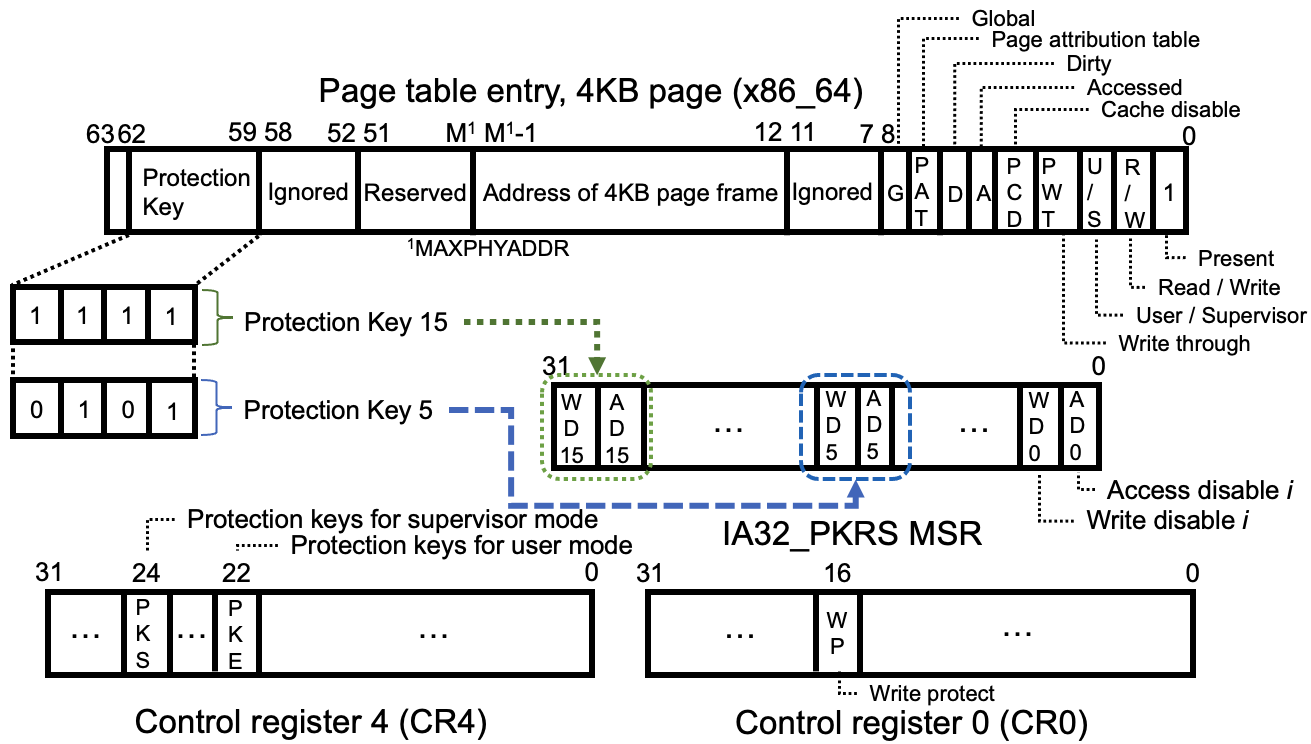
\includegraphics[bb=0 0 1311 744, scale=.200]{./imgs/002_screenshot_2021-07-26_19.13.09.png}
  \end{center}
  %  \vspace{-4.5ex}
% \vspace{-2.0ex}  
  \caption{
    %
    Intel memory protection key \cite{intel-mpk}
    %
  }
%  \vspace{-0.5ex}      
%  \ecaption{
%    Overview of software based side channel attack
%  }
  % \vspace{-3.0ex}
 \label{fig:mpk_overview}
\end{figure}



% \figref{fig:mpk_overview}に示す通り,
% %
% PTE において,4 bit の Protection key (Pkey) が割当てられており,16 個
% の Pkey を指定可能である.また,32 bit の読書き制限操作レジスタ(
%   Pkey あたり,Write disable(WD),Access disable(AD)の2 bit)を
% 介して,Pkey 単位で読書き制限の制御を行う.

% %{\it i}番目の
% Pkey {\it i}($0 \leq i \leq 15$)に対する読書き制限制御は,読書き制限
% 操作レジスタを介して行う.
% %
% {\it i} $\times$ 2のビット AD {\it i} の値が1の場合,読込み不可.0の
% 場合,読込み可,{\it i} $\times$ 2+1 のビットWD {\it i}+1が1の場合,
% 書込み不可,0の場合,書込み可とされる.

% MPKにおいて,読書き制限操作レジスタでの読込み制限,書込み制限は個別に
% 制御可能である.
% %
% また,複数のPTEに対して,Pkey を指定することで,読書き制限操作レジスタ
% を利用して一括に読書き制限制御を可能としている.
%
% 従来,PTE単位での読書き制御は読込みのみ,あるいは読書きの2種類を指定で
% きたが,MPKを用いることで読込み制限,書込み制限を個別に制御可能である.
% %
% また,Protection keyを複数のPTEに指定することで,読書き制限操作レジス
% タのみでの一括制御を可能としている.


% \begin{figure}[t]
%   \centering
%   \includegraphics[bb=0 0 1237 862, scale=.200]{./imgs/A01X_09_screen_shot_2021-12-17_15.29.59.png}
%     %  \vspace{-4.5ex}  
%   \caption{
%     %
%     Overview of privilege escalation and DoS
%     %
%   }
%   \label{fig:overview_kvuln}
% %\vspace{-5.0ex}        
% \end{figure}


% \begin{table}[t]
%   \centering
% \caption{
% %
%   %The comparison of feature among Blockchain.info, WalletExplorer.com, Bitiodine, and our proposed system.
%   %
%   Available PoC code for Linux kernel vulnerability list.
%   DoS: denial-of-service, Mem. Corr.: Memory Corruption
%   %among existing systems and proposed system
%   %
%   % CVE-2017-1000112
%   % https://www.exploit-db.com/exploits/43418
%   % CVE-2017-7533
%   % https://www.exploit-db.com/exploits/44302
%   % CVE-2016-9793
%   % https://www.exploit-db.com/exploits/41995
%   % CVE-2016-4997
%   % https://www.exploit-db.com/exploits/40435
% }
% %  \vspace{-0.5ex}  
% \scalebox{1.0}{
% \begin{tabular}{lll}
% %\hline
% \hline \noalign{\smallskip}
% \begin{tabular}{c}
%   {\bf CVE ID}
% \end{tabular}
% &
% \begin{tabular}{c}
%   {\bf Types}
% \end{tabular}
% %& {\bf PoC} & {\bf Publish Date} &
% &
% \begin{tabular}{c}
%   {\bf Description}
% \end{tabular}  
%     \\
%        \noalign{\smallskip}
%        \hline
%        \noalign{\smallskip}
%        CVE-2016-4997\cite{CVE-2016-4997} & DoS, Mem. Corr. & Boundary check error\\% in setsockopt implementation\\
%        CVE-2016-9793\cite{CVE-2016-9793} & DoS, Mem. Corr. & Boundary check error\\% in net/core/sock.c\\
%        CVE-2017-6074\cite{CVE-2017-6074} & DoS & Use after free\\% in net/core/sock.c\\                     
%        CVE-2017-7533\cite{CVE-2017-7533} & DoS, Mem. Corr. & Race condition\\% in the fsnotify implementation \\
%        CVE-2017-16995\cite{CVE-2017-16995} & DoS, Mem. Corr. & Boundary check error\\% in kernel/bpf/verifier.c\\% occurs memory corruption.\\
%        CVE-2017-1000112\cite{CVE-2017-1000112} & Mem. Corr. & Race condition\\% in net/ipv4/ip\_output.c\\

% \hline
% \end{tabular}
% }
% \label{tb:kernel_vulnerability_list}
% %\vspace{-1.0ex}  
% \end{table}


% \begin{figure*}[t]
%   \begin{center}
%     %\includegraphics[bb=0 0 1254 835, scale=.240]{./imgs/003_screen_shot_2019-08-14_17.12.23.png}
%     \includegraphics[bb=0 0 1581 882, scale=.240]{./imgs/A01X_01_screenshot_2021-09-17_21.18.21.png}
%   \end{center}
% %  \vspace{-1.0ex}
%   \caption{
%     %
%     Overview of the vulnerable kernel code tracer (vkTracer)
%     %
%   }
% %  \vspace{-2.0ex}
%   %\label{fig:restriction_approach_applying}
%   \label{fig:approach_overview}
% %  \vspace{-2.0ex}
% \end{figure*}



\subsection{Kernel Vulnerability}
% カーネル脆弱性は,カーネルへの攻撃に利用可能とされる実装不備とされる
% \cite{chen11linux}.
% %
% 特権奪取攻撃では,カーネル脆弱性を利用して任意のコードを挿入し,カーネ
% ルにおける権限操作を行うカーネル関数\verb|commit_creds| および
% \verb|prepare_kernel_cred|の呼出しによる権限情報の変更
% \cite{CVE-2016-4997,CVE-2016-9793,CVE-2017-1000112},または,カーネル
% 仮想記憶空間上の権限情報を格納するカーネルデータの変数\verb|cred|を改
% ざんし,ユーザプロセスのユーザIDを管理者ユーザへ変更する
% \cite{CVE-2017-16995}.

% 特権昇格攻撃,およびカーネルの提供するセキュリティ機能に対する無効化攻撃では,
% カーネルへの攻撃に利用可能とされる実装不備であるカーネル脆弱性のなかでも,カーネ
% ル脆弱性を介した任意のカーネルコードの挿入,実行によるメモリ破壊攻撃が利用される
% \cite{chen11linux}

% Linux カーネルにおいて,全てのユーザプロセスは同一のカーネルの仮想記憶空間を利用
% している.攻撃の起点となるカーネル脆弱性と共通の仮想記憶空間に存在するカーネル
% コード,およびカーネルデータは,仮想アドレスを指定し参照可能であり,メモリ破壊攻
% 撃に成功した場合,任意のカーネルデータは改ざん可能となる.
% %
% In the Linux kernel, all user processes use the same kernel virtual memory
% space. The kernel code and kernel data in the virtual memory space common to the
% kernel vulnerability that is the starting point of the attack can be referenced
% by specifying a virtual address, and the memory corruption attack If the attack
% succeeds, any kernel data can be tampered with.

%Kernel vulnerabilities are types of improper implementations that lead to kernel
Kernel vulnerabilities are improper implementations that lead to kernel
attacks \cite{chen11linux}.
% 特権昇格攻撃では,カーネルにおける権限操作を行うカーネル関数を強制的に呼出し,権
% 限情報が変更される \cite{CVE-2016-4997,CVE-2016-9793,CVE-2017-1000112}.また,権
% 限情報を格納するカーネルデータの変数 \verb|cred| を改ざんし,ユーザプロセスのユーザ ID
% を管理者ユーザへ変更する \cite{CVE-2017-16995}.
% perform the modification
Privilege escalation forcibly invokes kernel codes that modify privileged
information \cite{CVE-2016-4997,CVE-2016-9793,CVE-2017-1000112}. 
% privilege operations in the kernel and 
Specifically, the variable \verb|cred| of the kernel data that stores privileged
information is overridden from the normal user to the administrator
\cite{CVE-2017-16995}.
% with, and 

% セキュリティ機能である強制アクセス制御の無効化攻撃では,カーネルにおける強制アク
% セス制御を管理する関数ポインタの一覧\verb|selinux_hooks|の一部を強制アクセス制御
% を回避するカーネル関数へのポインタへ変更し,セキュリティ機能の無効化を行う
% \cite{nexus5exploit,grsecurity}.
% %
% 強制アクセス制御が無効化された場合,管理者権限の制限は行われない.特権奪取攻撃と
% 組み合わせることで,管理者権限を自由に利用可能となる.
% In the attack to security feature, 
The defeat of the MAC forcefully modifies the list of function pointers that
manage the access control decisions in the kernel. Meanwhile, the variable
\verb|selinux_hooks| that stores function pointers, is modified to the inserted kernel 
%are changed to inserted kernel
codes that bypass the access control \cite{nexus5exploit,grsecurity}.
% , thereby disabling the security feature

% When the mandatory access control is disabled, no restrictions for
% administrative privilege. 
The combination of privilege escalation and the MAC being disabled provides full
administrator capability to the adversary with no restrictions on the kernel.
%achieves 
% lead 
% privileges can be used freely.
\begin{table}[t]
    \centering
    %\caption{Chen らによるカーネルの脆弱性を用いた攻撃の影響種別 \cite{chen11linux}}
    %\caption{Affection of kernel vulnerability attack \cite{chen11linux}.}
    \caption{Top CWE of kernel memory vulnerability \cite{nvd} %\cite{chen11linux}
    }
    % ($\checkmark$ is supported; $\triangle$ is partially supported)}
    \scalebox{0.62}{  
    \begin{tabular}{llcc}
      %  \hline
        \hline \noalign{\smallskip}
      %  \hline
      \begin{tabular}{c}
        {\bf Type}
      \end{tabular}
      &
      \begin{tabular}{c}
        {\bf Content}
      \end{tabular}
      &
      \begin{tabular}{c}
        {\bf CVE}
      \end{tabular}
      &
      \begin{tabular}{c}
        {\bf PoC}
      \end{tabular}
      \\
       %影響                  & 内容\\
    %    Types             & Content & CVE & PoC\\
       \hline \noalign{\smallskip}
      %  \hline
      CWE-200 	& Exposure of Sensitive Information to an Unauthorized Actor	&125	&6\\
      NVD-CWE-Other 	& Other	&87	&5\\
      CWE-119 	&Improper Restriction of Operations within the Bounds of a Memory Buffer	&82	&3\\
      CWE-401 	&Missing Release of Memory after Effective Lifetime	&78	&0\\
      CWE-399 	&Resource Management Errors	&52	&1\\
      CWE-20 	&Improper Input Validation	&44	&1\\
      CWE-787 	&Out-of-bounds Write	&31	&1\\
      CWE-416 	&Use After Free	&20	&0\\
      CWE-125 	&Out-of-bounds Read	&19	&1\\
      %CWE-362 	&Concurrent Execution using Shared Resource with Improper Synchronization ('Race Condition')	&18	&3\\
      CWE-362 	&Concurrent Execution using Shared Resource ('Race Condition')	&18	&3\\
      CWE-189 	&Numeric Errors	&17	&0\\
      CWE-264 	&Permissions, Privileges, and Access Controls	&17	&2\\
      CWE-190 	&Integer Overflow or Wraparound	&16	&0\\
      CWE-909 	&Missing Initialization of Resource	&14	&0\\
      CWE-400 	&Uncontrolled Resource Consumption	&12	&0\\
      CWE-772 	&Missing Release of Resource after Effective Lifetime	&11	&0\\
      NVD-CWE-noinfo 	&Insufficient Information	&11	&1\\
      \hline \noalign{\smallskip}
      Other CWE & Under 10 CVE & 70&3\\
      \hline \noalign{\smallskip}
      Total & & 724 & 27\\
      \hline \noalign{\smallskip}
    %   \hline

    %    Obtain Information & Information leakage from kernel & $\triangle$\\
    %    Gain Privilege & Taking of administrator privilege   & $\checkmark$\\
    %    Bypass a Restriction & Evading of access control decision & $\checkmark$\\
    %    Overflow & Overwriting of stack or heap region & $\checkmark$\\
    %    Denial of Service & Forcing kernel to stop running & $\checkmark$\\
    %    Memory Corruption & Overwriting or reading of kernel code / data on virtual memory & $\checkmark$\\
      %  Memory corruption  & Overwriting or reading of kernel code / data on virtual memory & $\checkmark$\\
      %  Policy violation   & Miss implementation of access control decision & $\checkmark$\\
      %  Denial of Service  & Forcing kernel to stop running & $\checkmark$\\
      %  OS information leakage  & Information leakage from uninitialized data variables & $\triangle$\\
    %    \hline
    \end{tabular}
  }
    \label{tb:kernel_vulnerability_affection}
  \end{table}
  
  \begin{table}[t]
    \centering
  \caption{
  %
    %The comparison of feature among Blockchain.info, WalletExplorer.com, Bitiodine, and our proposed system.
    %
    % Available PoC code for Linux kernel memory vulnerability list
    Executable PoC code for Linux kernel memory vulnerability list
    ($\checkmark$ is protection available;)
    % $\triangle$ is partially supported)
    % DoS: Denial of Service, Mem. Corr.: Memory Corruption
    %among existing systems and proposed system
    %
    % CVE-2017-1000112
    % https://www.exploit-db.com/exploits/43418
    % CVE-2017-7533
    % https://www.exploit-db.com/exploits/44302
    % CVE-2016-9793
    % https://www.exploit-db.com/exploits/41995
    % CVE-2016-4997
    % https://www.exploit-db.com/exploits/40435
  }
  %  \vspace{-0.5ex}  
  \scalebox{0.75}{
  \begin{tabular}{lllc}
  %\hline
  \hline \noalign{\smallskip}
  \begin{tabular}{c}
    {\bf CVE ID}
  \end{tabular}
  &
  \begin{tabular}{c}
    {\bf CWE}
  \end{tabular}
  &
%   \begin{tabular}{c}
%     {\bf Types}
%   \end{tabular}
  %& {\bf PoC} & {\bf Publish Date} &
%   &
  \begin{tabular}{c}
    {\bf Description}
  \end{tabular}  
  &
  \begin{tabular}{c}
    {\bf KDPM}
  \end{tabular}  
      \\
         \noalign{\smallskip}
         \hline
         \noalign{\smallskip}
         CVE-2016-4997\cite{CVE-2016-4997} & CWE-264 & Boundary check error in setsockopt function & $\checkmark$\\
         CVE-2016-9793\cite{CVE-2016-9793} & CWE-119 & Boundary check error in net/core/sock.c & $\checkmark$\\
        %  CVE-2017-6074\cite{CVE-2017-6074} & & DoS & Use after free\\% in net/core/sock.c\\                     
        %  CVE-2017-7533\cite{CVE-2017-7533} & DoS, Mem. Corr. & Race condition\\% in the fsnotify implementation \\
         CVE-2017-16995\cite{CVE-2017-16995} & CWE-119 & Boundary check error in kernel/bpf/verifier.c & $\checkmark$\\
         % occurs memory corruption.\\
         CVE-2017-1000112\cite{CVE-2017-1000112} & CWE-362 & Race condition in net/ipv4/ip\_output.c & $\checkmark$\\

        %  CVE-2016-4997\cite{CVE-2016-4997} & CWE-264 & DoS, Mem. Corr. & Boundary check error in setsockopt function\\
        %  CVE-2016-9793\cite{CVE-2016-9793} & CWE-119 & DoS, Mem. Corr. & Boundary check error in net/core/sock.c\\
        % %  CVE-2017-6074\cite{CVE-2017-6074} & & DoS & Use after free\\% in net/core/sock.c\\                     
        % %  CVE-2017-7533\cite{CVE-2017-7533} & DoS, Mem. Corr. & Race condition\\% in the fsnotify implementation \\
        %  CVE-2017-16995\cite{CVE-2017-16995} & CWE-119 & DoS, Mem. Corr. & Boundary check error in kernel/bpf/verifier.c\\% occurs memory corruption.\\
        %  CVE-2017-1000112\cite{CVE-2017-1000112} & CWE-362 & Mem. Corr. & Race condition in net/ipv4/ip\_output.c\\  
  \hline \noalign{\smallskip}         
%   \hline
  \end{tabular}
  }
\label{tb:kernel_vulnerability_list}
\end{table}


% Kernel misimplementations result in kernel vulnerabilities, which can
% eventually lead to kernel attacks \cite{chen11linux}.
% %
% A kernel attack can lead to several types of damages to the running
% kernel.
% %
% Figure \ref{fig:overview_kvuln} shows that typical attacks include privilege
% escalation through memory corruption, which can lead to administrator privileges
% (e.g., root account) and DoS through unusual kernel data modification, defeating
% the stability of the kernel \cite{chen11linux}.

% \subsection{PoC Codes}
% %
% Several kernel vulnerabilities have been reported for Linux kernels
% \cite{cvedetails}.
% %
% PoC codes are small programs that directly invoke
% vulnerable kernel codes to exploit a known vulnerability.
% %
% Table \ref{tb:kernel_vulnerability_list} summarizes some of the available PoC
% codes. These include the execution techniques to invoke vulnerable kernel code
% in a specific version of the Linux kernel.
% %
% In this study, several kernel vulnerabilities are applied for the
% evaluation of vkTracer:

% \begin{itemize}

% %\item {\bf Memory corruption}: This overwrites the memory region of the
% \item {\bf Privilege escalation}: This overwrites credential
%   information through the corruption of stack or heap areas
%   and exploits a kernel vulnerability to achieve privilege
%   escalation.
%   %or defeat security mechanisms.

% \item {\bf DoS}: This leads to unstable behavior that forcibly terminates the
%   running kernel. A system becomes vulnerable to DoS attacks because a variable
%   is accessed or freed after its memory has already been freed (known as a
%   use-after-free (UAF) vulnerability), deadlock of mutual exclusion, or finite
%   loops when the flag control fails.

%   %% It leads unstable behavior to forcibly terminate the running kernel.
%   %% %
%   %% DoS was attracted from variable access after the it is freed (known
%   %% as use after free (UAF)) , dead lock of mutual exclusion, or finite
%   %% loop when the failing of flag control.

  
%   %% It overwrites the memory region of stack or
%   %% heap area that exploits kernel vulnerability to achieve privilege
%   %% escalation or defeating security mechanism.
  
%   %UAF is a
%   %Additionally,  is also occurs the DoS for the kernel.
  
%   %Critical section 
%   %The a variable access after the it is freed.
%   %The kernel referred the undefined value that 
%   %Use After Free (UAF): It is 

% %% \item Critical section: It is finite loop when the failing of flag control
% %%   or dead lock of mutual exclusion that laeds DoS for the running kernel.
  
% %% \item バッファオーバーフロー:スタック領域あるいはヒープ領域の上書きが
% %%   行われる.バッファオーバーフローにより,権限情報が改竄された場合,特
% %%   権奪取に繋がる.

% %% \item 解放済みメモリの参照(Use-After-Free):解放済みメモリ領域の参照
% %%   が行われる.不定な値の読込みと利用によりカーネル動作が不定となり,
% %%   DoS に繋がる.

% %% \item 競合条件の発生:フラグ操作処理の誤りによる意図的な無限ループやデッ
% %%   ドロックの発生が行われる.カーネル動作の処理待ちが発生し,DoS に繋が
% %%   る.

% %\item 脆弱性4:xxx
% \end{itemize}



%% The effect of kernel attack has several types of damage for the running kernel.
%% %
%% Typical attacks are memory corruption that occurs a privilege escalation
%% of the administrator capability (e.g., root account) and denial of
%% service (DoS) that defeats the stability behavior of kernel
%% \cite{chen11linux}.

%
  %
%% \blueuline{The memory corruption demonstrates that a vulnerable kernel
%%   code directly modifies the kernel code or kernel data in the kernel
%%   address space to take the privilege capability (e.g., administrator
%%   account) in } \cite{chen11linux}.
%% %
%% Figure \ref{fig:vmemory_and_attack}
%% \blueuline{
%%   indicasts the attack regions of the memory corruption that
%%   achieves a privilege escalation attack.
%%   %
%%   }
%% An adversary's user process requires the overwriting of \reduline{kernel data that
%% contains} \verb|UID| variable of the user identifier in the kernel address space.
%% %
%% %To achieve a privilege escalation attack through kernel memory
%% %corruption,

%% %
%% Latest Linux kernel adopts MAC of the Linux security module (LSM) to
%% restrict the privilege capability of the administrator.
%% %
%% \reduline{To avoid MAC restriction, the adversary's user process
%%   utilizes the memory corruption vulnerability} to also replace LSM's
%% kernel code of \verb|security_hook_list| with the non-checking access
%% control kernel code in \cite{nexus5exploit,grsecurity}.

%% \begin{figure*}[t]
%% %  \begin{center}
%%   \centering
%%   \hspace*{-4.5ex}
%%     %\includegraphics[scale=.275]{./imgs/002_screen_shot_2019-08-04_15.19.54.eps}
%%     \includegraphics[bb=0 0 1502 564, scale=.240]{./imgs/Z002_screenshot_2020-05-22_17.44.30.png}
%% %  \end{center}
%% %  \vspace{-1.0ex}
%%   \caption{
%%     %
%%     Page table management of virtual address in \cite{oreilly} and physical address with attack regions
%%     %
%%   }
%% %  \vspace{-2.0ex}  
%%   \label{fig:vmemory_and_attack}
%% %  \vspace{-2.0ex}
%% \end{figure*}

%% \subsection{Address Space and Page Table}
%% %
%% %shows that the page table maintains page entry assignments, which
%% %allocates relationships between the physical and virtual addresses for
%% %each page of the page table.
%% %
%% \blueuline{[N-03]
%%   Modern kernels and hardware support the page table structure to provide virtual memory
%%   larger than the physical memory.
%%   %
%%   As depicted in Figure \ref{fig:vmemory_and_attack}, the page table
%%   structure that creates virtual address spaces.
%% %
%% %
%%   More especially, the page table structure (e.g., 4 / 5 level paging
%%   on x86\_64) maintains page and page table entry, which indicates
%%   relationships between the virtual and physical addresses. Additionally, The CR3
%%   register stores the virtual address of the page table on the x86\_64
%%   architecture in} \cite{intel}.
%%   %

%% \blueuline{  
%% Linux provides the address space of virtual memory is separated into
%% two regions for the user and kernel modes in} \cite{oreilly}.
%% %
%% %
%% %
%% %More especially, Linux has a multiple-page table structure that creates virtual address
%% %It can be used to change a virtual address (48 bits on x86\_64) to a
%% %Linux It can be used to change a virtual address (48 bits on x86\_64) to a
%% Linux assigns a virtual address (48 bits on x86\_64) to a physical
%% address on the page table.
%% %
%% The smallest set is a page (4 KB on x86\_64).  The Linux kernel page
%% stores the kernel code and kernel data in the specific virtual address
%% space of \reduline{kernel page} for the kernel mode.
%Kernel memory corruption is a type of kernel vulnerability that leads
%to the privilege escalation attack \cite{chen11linux}.
%
%The list of CVE \cite{cvedetails} \blueuline{registers 2,708 Linux kernel
%vulnerabilities.}
%
%% \reduline{
%%   The one of typical kernel vulnerability is memory corruption that is reported
%%   140 reports are discovered in}
%% \cite{cvedetails}
%  Kernel miss implementations covers the kernel vulnerability that
%  leads to the kernel attack 
% The potential effects of 
%capability (e.g., root account), and denial of service (DoS), which
%achieve the kernel exploiting through a
%
%some kernel vulnerabilities
% as follows:
%% In this paper introduce the demonstrated several kernel
%% vulnerabilities for the evaluation of vkTracer as following: 


% # -*- coding: utf-8 -*-
% \section{Precondition} \label{seciton:threatmodel}
\section{Threat Model} \label{seciton:threatmodel}
\subsection{Environment}
% 提案するセキュリティ機構の想定する脅威モデルとして,攻撃者の目標は特権
% 奪取とする.
% %
% 攻撃シナリオとして,攻撃者はカーネル脆弱性を利用するユーザプロセスを実
% 行し,脆弱なカーネルコードから権限変更を行うカーネル関数の呼出し,また
% は権限情報の改ざんを行い,特権奪取を試みる.
% %
% 脅威モデルの利用環境において,提案するセキュリティ機構を用いることで攻
% 撃シナリオに沿った攻撃者の特権奪取攻撃の防止を行う.
% %
% 脅威モデルにおける攻撃者の要件,および利用環境を以下にまとめる.


% 本稿において,提案するセキュリティ機構の想定する脅威モデルとして,攻撃者の目標は
% 特権奪取およびカーネルの提供するセキュリティ機能の無効化とする.
% In this paper, the 
We assumed a threat model for the KDPM.
%
The adversary acquires administrator privileges and disables the MAC in the
target environment as follows:

% \subsection{攻撃対象環境}
% 想定する脅威モデルにおける攻撃者および攻撃対象環境は以下とする.
% The attacker and target environment in the assumed threat model are as follows.

\begin{itemize}%[topsep=0pt]%\topsep=-1.0ex \itemsep=-1.0ex \parskip=1.0ex
  \item Adversary: An adversary gains normal user privileges, attempts
  privilege escalation, and defeats the MAC via the PoC code that exploits kernel
  vulnerabilities.
% \item 攻撃者: 一般ユーザ権限にて,カーネル脆弱性を利用するPoCコードを
%   介して特権奪取およびセキュリティ機能の無効化を試行可能.
% \item 攻撃者: 一般ユーザにて,特権奪取可能なカーネル脆弱性を利
%   用するPoCコードをユーザプロセスとして実行.

\item Kernel: A kernel contains kernel vulnerabilities that can be exploited for
privilege escalation and defeating the MAC. Existing security
mechanisms (e.g., KCoFI, KASLR, and AKO) are not applied.
% Security features (e.g., forced access control) are provided enabled. 

% \item カーネル:特権奪取とセキュリティ機能の無効化に利用可能なカーネル脆弱性を含
%   む.セキュリティ機能(例,強制アクセス制御)は有効化して提供する.
% \item カーネル:特権奪取攻撃に利用可能なカーネル脆弱性を含む,既存のセ
%   キュリティ機構(例,KASLR,CFI,およびAKO)の適用は行わない.

  \item Kernel vulnerability: A kernel vulnerability is the presence of a vulnerable
  kernel code that exploits kernel memory corruption.
  %  kernel vulnerability invoked by a user process run by an attacker. The vulnerable kernel code can write to
  % any virtual address.
% \item カーネル脆弱性:攻撃者の実行するユーザプロセスより呼出されるメモリ破壊可能
% なカーネル脆弱性.脆弱なカーネルコードから任意の仮想アドレスに対して,書込み可
% 能.
% \item カーネル脆弱性:攻撃者を行うユーザプロセスより特権奪取に利用可能
%   なカーネル脆弱性.脆弱なカーネルコードから任意の仮想アドレスを指定し,
%   権限変更を行うカーネル関数を呼出し可能.また,権限情報情報を含むカー
%   ネルコードへの書込みが可能.

  \item Attack targets: Attack targets are kernel data related to
  privileged information of user process (e.g., user id) and kernel data of the MAC (e.g., function
  pointers and access policies).
% \item 攻撃対象:カーネルデータのうち,ユーザプロセスの権限情報,およびセキュリ
% ティ機能に関するカーネルデータ.
% \item 攻撃対象: 特権奪取攻撃を行うユーザプロセスの攻撃対象は権限情報
%   の仮想アドレス(例.ユーザプロセスの権限情報).

\end{itemize}


% \subsection{Environment}

% The assumed environment of vkTracer involves an adversary that attempts
% to access vulnerable kernel codes using a PoC code.
% %
% vkTracer assumes this environment in preparation for an eventual
% deployment to a production environment. This environment, involving
% the adversary and kernel capability, comprises the following:

% %\vspace{-1.2ex}    
% \begin{itemize}%\itemsep=-1.0ex \parskip=1.0ex

% \item {\bf Adversary}:
% An adversary uses a normal user account and PoC codes that exploit kernel vulnerabilities.

% \item  {\bf Kernel}:  
% A kernel contains kernel vulnerabilities, which are directly used by
% PoC codes. A kernel provides internal tracing features for kernel
% code invocation, static kernel image, and debug information.

% \item {\bf Kernel vulnerability}: A kernel vulnerability that has already
%   been discovered or demonstrated. Vulnerable kernel codes are
%   identified as a known piece of kernel vulnerability.

% \end{itemize}
%\vspace{-1.2ex}

\subsection{Scenario} \label{subsection:attack_scenario}
% \subsection{攻撃シナリオ}
% 想定する攻撃者の攻撃シナリオは,攻撃対象となるカーネルに対して,カーネル脆弱性を
% 利用するPoCコード利用するユーザプロセスを実行し,脆弱なカーネルコードを介するこ
% とで攻撃対象の改ざんを行う.
The adversary induces the attack that executes the PoC code as the user
process exploits the vulnerable kernel code. 
%
The following are the details of an attack:
% More specifically, 
% a kernel vulnerability 
% against the target kernel. 
% The attack target is then tampered with via the vulnerable kernel code.
% %
% 例として,強制アクセス制御の無効化攻撃では,アクセス制御箇所を関数ポインタの改ざ
% んにより,アクセス制御判定を行わないカーネルコードへ置換える.
% %
% カーネルの提供する強制アクセス制御が働かなくなることから,管理者権限への制限を排
% 除する.その後,特権奪取攻撃により,ユーザ権限を管理者権限に書換え,計算機の完全
% な制御を可能とする.
%%%%%%%%%
% More specifically, the user process of the adversary forcefully disables MAC
% by replacing the function pointer of the kernel code with one that does not
% make access decisions; and
%
% then rewrites user privileges to administrator privileges, enabling full control
% of the computer.
%%%%%%%%%%%%%
% , thereby eliminating restrictions on administrative
% privileges. 
% privilege escalation attack

\begin{enumerate}%[topsep=0pt]%\itemsep=-1.0ex \parskip=1.0ex  
  \item Privilege escalation attack\\
    %
    The user process of the adversary forcefully rewrites user privileges to
    gain administrator privileges for attaining full control of the computer.
  \item Defeating security mechanisms\\
    %
    The user process of the adversary forcefully disables the MAC by replacing the
    function pointer of the kernel code with one that does not make access
    decisions.

  
\end{enumerate}


% As an example, 
% in a forced access control override attack, the access control
% point is replaced with kernel code that does not make access control decisions
% by tampering with the function pointer.
% The kernel-provided 


% \subsection{Scenario} \label{subsection:attack_scenario}
% In the assumed scenario, vkTracer prepares the tracing and
% identification of the vulnerable kernel code.
% %
% First, vkTracer attaches to the PoC code of an adversary's user
% process, which accesses and executes the invocation of the vulnerable
% kernel code. 
% %
% %

% If successful, the adversary's user process can subsequently cause damages,
% including privilege escalation via memory corruption and DoS via UAF or critical
% section on the running kernel.
% %
% vkTracer forcibly hooks on to the vulnerable kernel code during the kernel
% attack process.
% %
% Then, vkTracer gathers the entire vulnerable kernel code invocation
% list from the tracing environment.
% %
% Finally, vkTracer generates the profile of vulnerable kernel code
% information (e.g., virtual address range and kernel function name).

%In the tracing and identification scenario, vkTracer prepares the

  %  An adversary uses normal user account and the PoC codes that exploit kernel vulnerabilities.

  %\blueuline{the PoC code that
   % exploits} kernel vulnerability \blueuline{to achieve the privilege
  %escalation attack}.

  %% A kernel contains the kernel vulnerabilities that are
  %% directory used from the PoC codes. A kernel provides internal tracing
  %% feature of kernel code invocation, static kernel image, and debug information.

  %% the sharing of the kernel address space for
  %% every user process.  \blueuline{The kernel address space contains the vulnerable kernel
  %% code, attack target kernel data.}
  %code, attack target kernel code, and kernel data.

%  It is already discovered or demonstrated kernel vulnerability.
  %  A vulnerable kernel code is identified as a known piece of kernel vulnerability.
  
  %
  %\blueuline{The PoC code as an user process that invokes the vulnerable kernel code.}
  %
  %It modifies any kernel code or kernel data that is present in the
  %kernel address space to lead the privilege escalation attack.}

%% \item {\bf Attack target}: It contains the security feature of 
%%   %\reduline{the kernel data or the parts of} kernel code (i.e., \reduline{an access control policy and
%%   \reduline{the kernel data of} kernel code (i.e., \reduline{an access control policy and
%%     an function pointer of} MAC)
%%   and privilege information of kernel data (i.e., user identifier).
%%   %
%%   These are the key points of the administrator's privilege
%%   restriction on the kernel.
  %


%after the adversary's user process attains administrator
%privilege or the kernel is stopped in the tracing environment.

%% The tracing scenario of vkTracer to achieve the
%% tracing and identifying of vulnerable kernel code.
%% %
%% vkTracer attaches the PoC code of adversary's user process that
%% accesses and executes the invocation of vulnerable kernel code.
%% %
%% After that, the adversary's user process can lead memory corruption
%% for the privilege escalation and UAF or critical section for the DoS
%% on the running kernel.
  
%% %
%% Subsequently, vkTracer forcibly hooks the vulnerable kernel codes
%% while the process of kernel at
%% %
%% Finally, vkTracer gathers the whole of vulnerable kernel
%% code list after the adversary's users process has administrator
%% privilege or the stopping of kernel in the tracing environment.

%that modifies the
%privilege information of the kernel data for privilege escalation.

%  the privilege escalation
%  that requires kernel memory corruption.
%Therefore, the adversary's user process alters the security features
%of the kernel code \blueuline{to defeat the administrator privilege restriction.}
%

%% \subsection{Preparation}
%% \blueuline{
%%   The preparation of the KPRM's resilience that 
%%   requires the two building process collects the necessary information
%%   to protect security features and privilege information
%%   from the attack scenario on the attack environment.
%% }

%% %
%% \reduline{  
%%   The building process, KPRM has prepared profiles of vulnerable kernel code
%%   information (e.g., virtual address range and kernel function name).
%%   %
%%   A tracing of KPRM traps PoC code execution to identify vulnerable kernel code
%%   to generate a profile.
%%   %
%%   %Moreover, attack target of kernel code and kernel data for the additional
%%   %Moreover, attack target of kernel data for the additional profiles information.
%%   Moreover, attack target of kernel data for the additional information.
%% }
%% %
%%   %KPRM has prepared a list of vulnerable kernel code, attack target of
%% %% \blueuline{  
%% %%   The remaining building process, KPRM has adopted profiles of kernel code to
%% %%   restrict vulnerable kernel code and protect attack target of kernel
%% %%   data at the KPRM kernel booting.
%% %% }
%% %% %
%% %% \blueuline{
%% %%   To cover the kernel attack from any user process,
%% %%   KPRM restricts all user processes on the running kernel.
%% %% }
%% %% %  that contain the  adversary's user process.
%% %% %Additionally, 
%% %% %
%% %% \blueuline{ KPRM supports a benign user process list that reduces the
%% %%   performance overhead for not malicious applications.
%% %%   %
%% %%   The administrator can manually register the flag of benign to avoid
%% %%   the restriction of KPRM after the execution of user process.
%% %% }

%% %
%% \reduline{
%% Additionally, the use case of KPRM assumes that building process is performed on the testing environment before the user deploys the KPRM for the production environment.
%% }



%To reduce the performance overhead, KPRM manages a benign user process
%list. It manually registers the flag of benign to avoid the
%restriction of KPRM for each user process on the running kernel.

%\subsection{Use case}
%% %
%% An tracing environment for vkTracer that requires an adversary should
%% access the vulnerable kernel code with PoC code.
%%   %
%% vkTracer assumes the tracing environment is performed on the
%% preparation before the deployment for the production environment.
%%   %
%% The tracing environment of adversary and kernel capability are as follows:
%}
  %preparation to prevents the an adversary's behavior with an attack
  %scenario.


% # -*- coding: utf-8 -*-
%\section{Design and Implementation} \label{section:approach}
%\section{Design of vkTracer} \label{section:approach}
\section{Design} \label{section:approach}

%\subsection{Design Concept} \label{subsection:design}
% \subsection{Concept} \label{subsection:design}
\subsection{Requirement} \label{subsection:design}
% 提案するセキュリティ機構の設計においては,カーネルにおいて,指定したカーネル
% データへの書込み制限を指定するため,次の要件を満たすことを目指した.

% 提案するセキュリティ機構では,システムコール毎に動作中のカーネルにおいて保護対
% 象カーネルデータに対して読書き制限を指定するため,設計として次の要件を満たすこ
% とを目指した.
% This study 
% To manage write restrictions on specified kernel data in the kernel, we designed
To manage write restrictions on specified kernel data, 
% we designed the KDPM to satisfy the following requirement: 
% we considered 
the KDPM should satisfy the following requirement: 
% in order to manage write restrictions on specified kernel data in the kernel.

% User processes rely on kernel features to control system resources and hardware
% (i.e., memory, file system, and network). These kernel features are constructed
% from a set of kernel codes, and system calls are used instead of user processes
% to invoke kernel codes at the kernel layer.  
% %
% This study designed vkTracer to achieve the following requirements for tracking
% the invocation of vulnerable kernel codes.

\begin{figure*}[tb]
  \hspace{10.0ex}
  % \begin{center}
  % \centering
  % 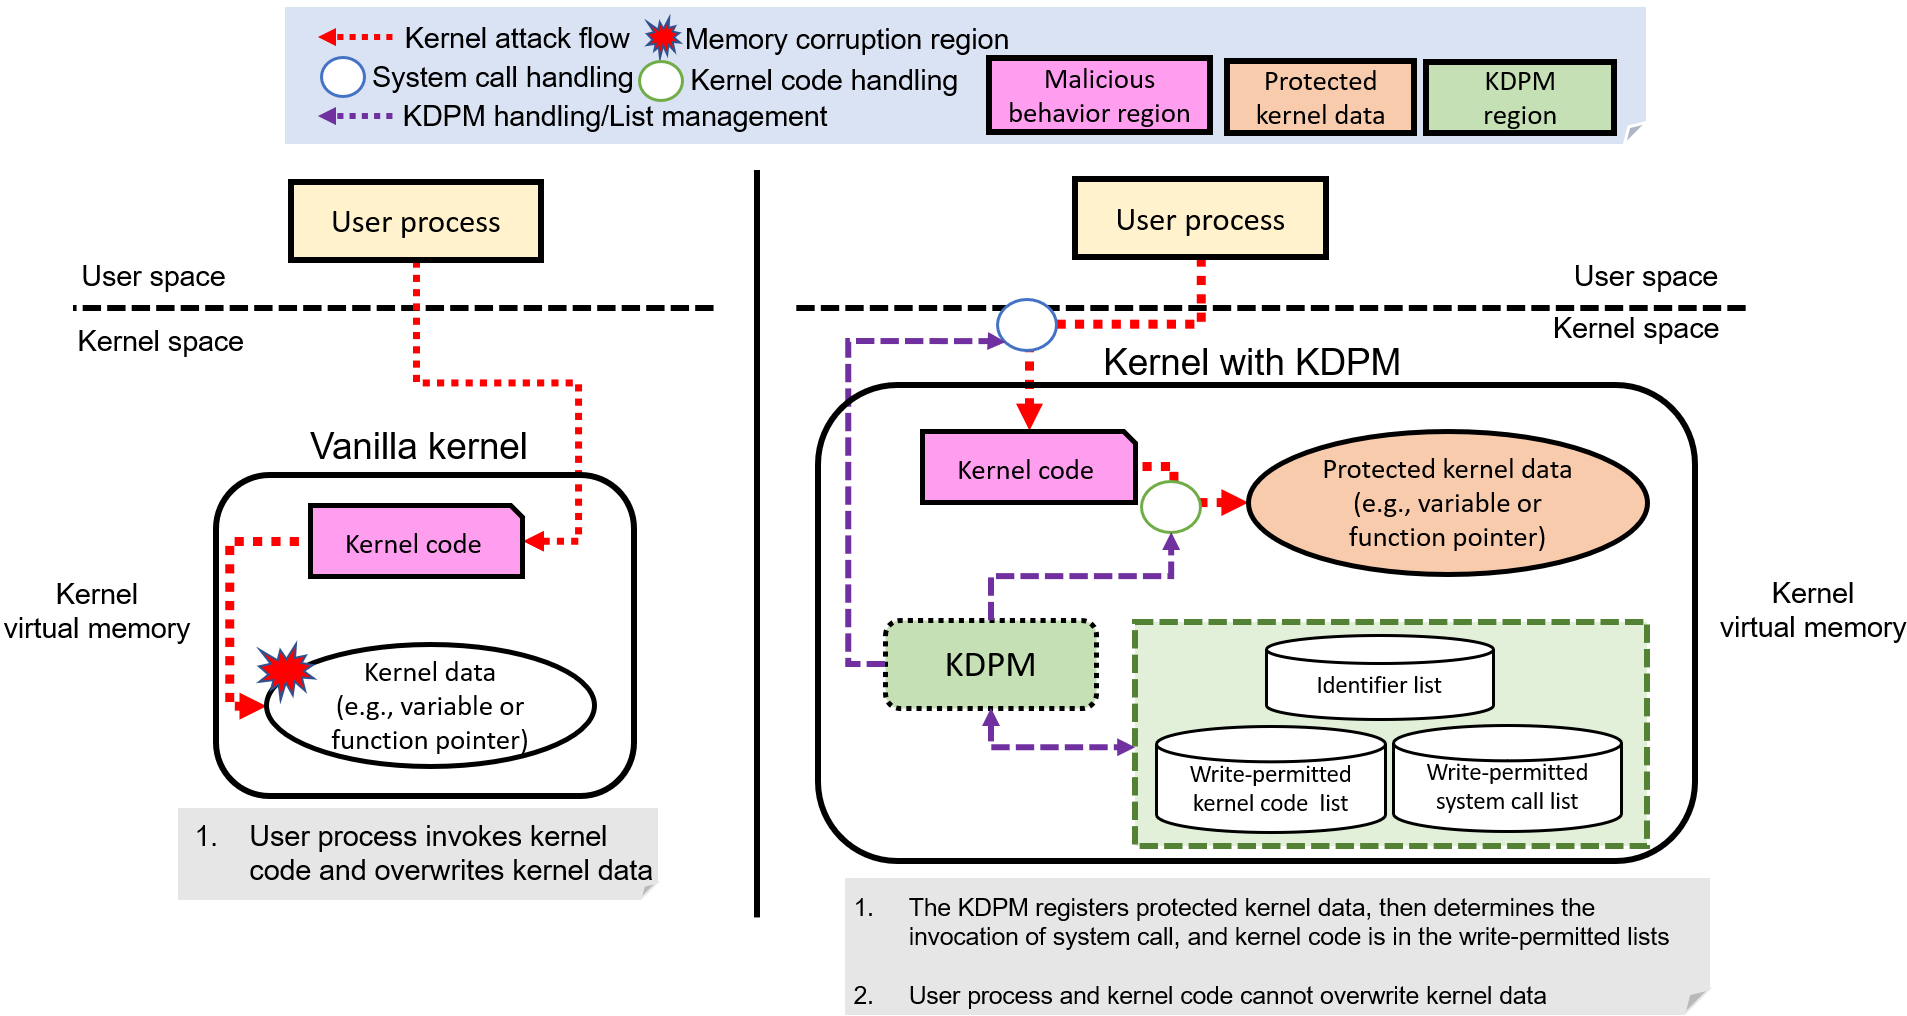
\includegraphics[bb=0 0 1587 852, scale=.280]{./imgs/003_screenshot_2021-07-27_19.37.39.png}
  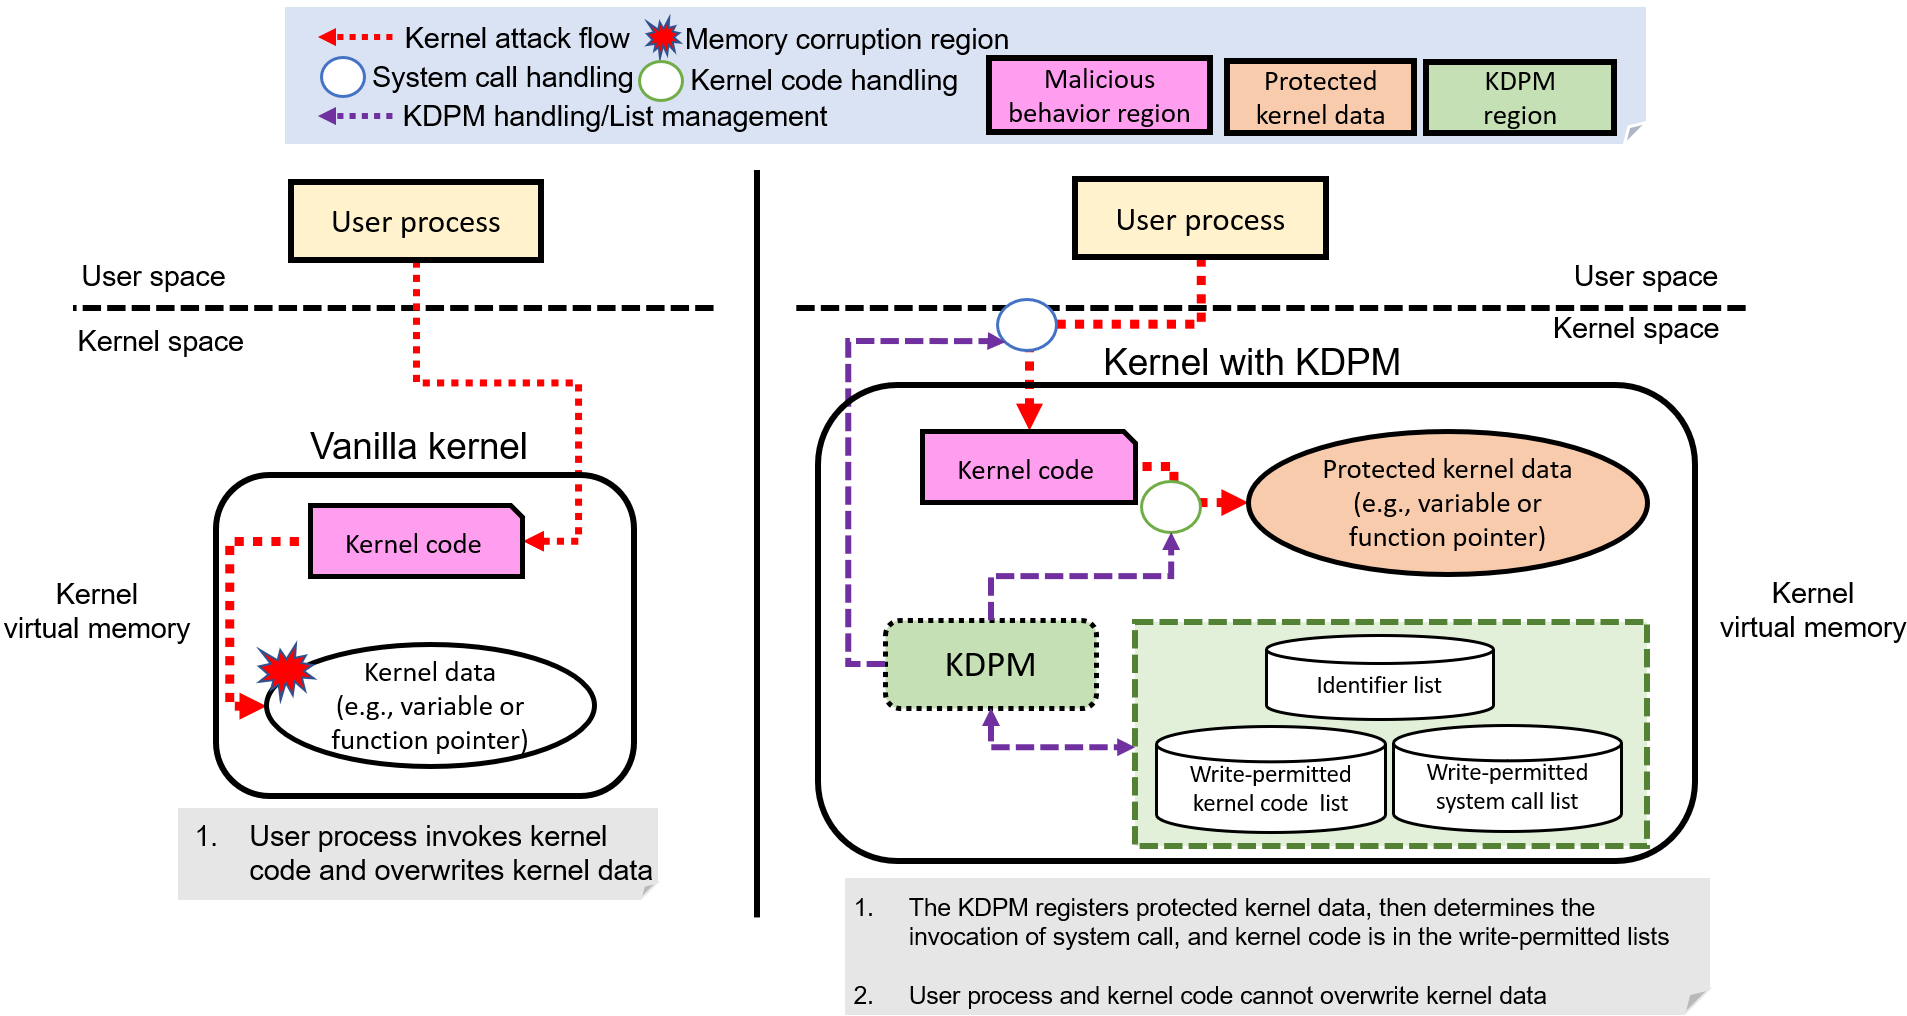
\includegraphics[bb=0 0 1430 762, scale=.320]{./imgs/003_screenshot_2021-07-27_19.37.39.png}
  % \end{center}
% \vspace{-1.5ex}      
  \caption{
    %
    %提案するセキュリティ機構の設計概要図
    Design overview of the KDPM
    %
  }
% \vspace{-0.5ex}      
% \vspace{-3.5ex}
 \label{fig:design_overview}
\end{figure*}


\begin{itemize}%\itemsep=-1.0ex \parskip=1.0ex
  % カーネル脆弱性を利用したカーネルデータの改ざんによる特権昇格,ならびにセキュ
  % リティ機能の無効化攻撃を緩和する.
  % %
  % カーネルデータに対する書込み制限の管理として,保護対象に指定したカーネルデー  
  % タ毎に書込み制限制御を特定のシステムコール単位,ならびにカーネルコード単位で
  % 処理可能とする.
  % %
  % 書込みを許可されたシステムコールに関するカーネルコード,ならびにカーネルコー
  % ドの実行中においてのみ保護対象に指定したカーネルデータへの書込みを可能とす
  % る.
\item {\bf Requirement}: Prevent privilege escalation and defeat of security mechanisms
 by illegally modifying kernel data via kernel vulnerabilities.
  %
  The kernel must control the write restrictions of kernel data for specific
  system calls and kernel codes on the running kernel.
  %
  The kernel data can be written only %during the invocation of 
  when system calls are invoked and the authorized kernel codes are executed.
% disablement attacks   
  % can be controlled 
    % for each kernel data specified as the target of  protection.
  % kernel code related to 
  %  to be written.

  % 攻撃を行うユーザプロセスによるカーネル脆弱性を利用したカーネルデータ
  % の改ざん(例,特権奪取攻撃)を想定し,保護対象カーネルデータの読書き
  % 制限を設定可能とする.
  % %
  % 動作中のカーネルにおける読書き制限の管理として,書込み制限の制御は
  % システムコール単位で処理する.
  % %
  % 読書き制限の切替えはシステムコール発行時に行い,書込みを許可され
  % るシステムコールの実行中においてのみ保護対象カーネルデータへの書込み
  % 制限を無効可能とする.


% \item Requirement 1 (R1): Trace the invocation of a
%   vulnerable kernel code that leads to memory corruption or DoS.
%   %
%   The tracing feature must trap the behavior of the adversary's user process and
%   kernel while the vulnerable kernel codes are invoked on the running kernel.

% \item Requirement 2 (R2): Identify the vulnerable kernel
%   code. 
%   %
%   The profile of the kernel vulnerability must contain the list of virtual address
%   ranges and function names. These are identified from the list of invoked
%   vulnerable kernel codes.
\end{itemize}

% \subsection{Challenges}

% vkTracer fulfills the requirements for identification and hooking the
% invocation of vulnerable kernel codes using a combination of tracing
% and restriction of the kernels.
% The challenges faced during the tracing and identification of vulnerable kernel codes
% are as follows:

% \begin{itemize}%\itemsep=-1.0ex \parskip=1.0ex
%   %
%   \item R1 raises the question of how to trace running kernel behavior during
%   an adversary's user process execution.
%   %
%   The attaching of the kernel is difficult from the user process, but kernel
%   features should introduce the hooking of all kernel code invocations.
%   %
%   This mechanism allows the tracing of entry points that can be registered to the
%   running kernel from the user process.  %when the adversary's

%   \item R2 raises the question of how to analyze the kernel structure with
%   the vulnerable kernel code invocation list.
%   %
%   The kernel should support symbol information for the running kernel and should
%   embed kernel component information into the static kernel image at the kernel
%   compilation time.
%   %
%   This mechanism allows an analysis of the relationship among the function
%   name, virtual address, and the invocated vulnerable kernel code for the profile
%   generation.

% \end{itemize}

\subsection{Design Overview}

KDPM fulfills the requirement for kernel data protection from the invocation of
vulnerable kernel codes. 
%
Figure \ref{fig:design_overview} outlines the design overview of 
% It is 
%
KDPM introduces the protected kernel data, identifier list, the
write-permitted system call list and write-permitted kernel code list.

%
% that stores the kernel data 
%the management of linking the identifier to the
KDPM manages the linking of the identifier that indicates the relationship between
the protected kernel data, write-permitted system call, and write-permitted kernel
code.
%
KDPM statically registers protected kernel data, identifiers of protected kernel
data, write-permitted system call, and write-permitted kernel code lists at the
source code. After that, KDPM dynamically controls the write restriction of
kernel data using identifier at the invocation of system call or kernel code for
the running kernel.

\subsection{Approach}
% 提案するセキュリティ機構として,要件を満たす設計概要を図
% \ref{fig:design_overview}に示す.
% %
% 提案するセキュリティ機構では,保護対象カーネルデータの書込み制限の制御に用いるために,
% 保護対象として指定するカーネルデータ(例,変数値,
% および関数ポインタ),ならびに識別子を設ける.
% そして,識別子をシステムコール,およびカーネルコードと紐付けて制御の管理を行う.

% 提案するセキュリティ機構の設計概要を\figref{fig:design_overview}に示す.
% 要件を満たすため提案するセキュリティ機構では,保護対象カーネルデータ
% (例,権限情報)を予め指定し,識別子を設けて管理する.また,システムコー
% ルと紐付け,保護対象カーネルデータの読書き制限を管理する.
%The KDPM supports the kernel data as protected kernel data (e.g., variable or
The KDPM supports specific kernel data as protected kernel data (e.g., variable
or function pointer) and the identifier to handle the write restrictions that
manages the write-permitted system calls and write-permitted kernel code.
%satisfy the aforementioned requirement.
%
% The proposed security mechanism defines and manages the following two types:
% system calls and kernel code.
%
% The following protected kernel data and identifier for restriction must be
% fulfilled:

% \subsubsection{保護対象カーネルデータ}
\subsubsection{Protected Kernel Data:}

The following are the definitions of protected kernel data and identifiers:
% to be managed by the proposed security
% mechanism 


% 提案するセキュリティ機構において管理する保護対象カーネルデータおよび識別子は次の
% 通りとする.

\begin{itemize}
% \begin{itemize}[topsep=0pt]%\topsep=-1.0ex \itemsep=-1.0ex \parskip=1.0ex%\topsep=-1.0ex \itemsep=-1.0ex \parskip=1.0ex
  
% \item 保護対象カーネルデータ:ユーザプロセスのカーネルデータ(例.権限情報),お
% よびカーネルにおけるセキュリティ機能において利用されるカーネルデータ(例.関数ポ
% インタ)
\item Protected kernel data: The kernel data of the user process (e.g.,
privileged information) and security mechanisms (e.g., the function pointer
and access policy).
% Kernel data of the user process (e.g., privileged information) and the kernel data of security mechanism (e.g., function pointer and access policy).
% in the kernel (e.g. (function pointer).

\item Identifier: The identifier is used to set the write restrictions of the
protected kernel data. For controlling the write restriction, the identifier is
associated with the protected kernel data, write-permitted system call, and
write-permitted kernel code.

% \item 識別子:保護対象カーネルデータの読書き制限を設定するために用いる識別子.書
%   込み制限制御のため,識別子に対し,保護対象カーネルデータ,および,書込み許可シ
%   ステムコール,書込み許可カーネルコードの紐付けを行う.
%   %書込み許可システムコール,書込み許可カーネルコードの紐付けを行う.
  
\end{itemize}


% 提案するセキュリティ機構を備えたカーネルでは,起動時に保護対象カーネル
% データと対応する識別子のリストを予め設ける.
% %
% 動作中のカーネルにおいて,保護対象カーネルデータはユーザプロセス毎に生
% 成されることを想定し,ユーザプロセスの起動時にて,識別子との関連づけを
% 行い,同時に読書き制限を設定する.
The kernel with the KDPM provides a list of protected kernel data and
corresponding identifiers in advance at the time of booting.
%
Additionally, the kernel data for each user process generation is assumed to be
protected.

% At the startup of the user process, the identifier is associated with the kernel
% data to be protected, and the read restriction is set at the same time.

% 提案するセキュリティ機構では,カーネル内部において,保護対象カーネルデータ,識別
% 子のリストを予め設ける.

% 提案するセキュリティ機構における保護対象カーネルデータおよび識別子は次
% の通りである.

% %\begin{itemize}
% \vspace{-2.0ex}
% \begin{itemize}\topsep=-1.0ex \itemsep=-1.0ex \parskip=1.0ex
% \item 保護対象カーネルデータの識別子:読書き制限を設定するために用いる
%   カーネルデータ種別を示す識別子.識別子に対して読書き制限の紐付けと設
%   定を行う.
  
% \item 保護対象カーネルデータ:アプリケーションをユーザプロセスとして実
%   行する際,カーネルにおいて設定されるカーネルデータ.
  
% \end{itemize}
% \vspace{-2.0ex}




%To satisfy the challenge of vkTracer, the enhancement of the
%capability for the kernel.
% vkTracer addresses the aforementioned challenges by enhancing the capabilities of
% the kernel.
% %
% Figure \ref{fig:approach_overview} outlines how vkTracer
% generates a profile by tracing the invocation of a vulnerable kernel
% code from the PoC code.
% %
% The following approach provisions for tracing and restriction must be
% fulfilled:


%\vspace{-1.0ex}    
% %\begin{itemize}%\itemsep=-1.0ex \parskip=1.0ex
% \begin{itemize}%[topsep=0pt,leftmargin=0.5cm]%\itemsep=-0.5ex
% \item {\bf Vulnerable kernel code dynamic tracing and analysis}\\
% %{\bf Vulnerable kernel code dynamic tracing and analysis}\\
% %The capability of 
% vkTracer provides a mechanism for dynamic kernel tracing and for the analysis of an
% adversary's user process (e.g., execution of PoC codes) in the running kernel.
% %
% vkTracer traps the invocation of vulnerable kernel codes that is
% requested when the adversary's user process attempts to exploit a
% kernel vulnerability.
% %
% Furthermore, this mechanism utilizes the symbol and debugging information of the
% static kernel image during tracing. This mechanism ensures that vulnerable
% kernel code information (e.g., virtual address range and function name) is used
% to generate a profile of a specific kernel vulnerability.


% \end{itemize}
%\vspace{-1.0ex}



% \subsubsection{読書き制限の管理と操作}
\subsubsection{Handling of Write Restrictions:}
% % \subsubsection{読書き制限の管理と制御}

% 提案するセキュリティ機構において,保護対象カーネルデータへの読書き制限制御は特
% 定のシステムコール,およびカーネルコードにて行う.
% %
% 提案するセキュリティ機構では,次の2種類を定義し,管理する.書込み制限の制御
% は,システムコールの発行時,ならびにカーネルコード実行時において書込み制御機能
% を呼出すことで行う.
The KDPM handles the write restrictions of the protected
kernel data using specific system calls and kernel codes.
%
The KDPM defines and manages the following:

%\begin{itemize}[topsep=0pt]%\topsep=-1.0ex \itemsep=-1.0ex \parskip=1.0ex%\topsep=-1.0ex \itemsep=-1.0ex \parskip=1.0ex      
\begin{itemize}
% \item 書込み許可システムコール:保護対象カーネルデータの書込み権限を有するシス
%    テムコール.
\item Write-permitted system call: A system call has write permission for
the protected kernel data.

% \item 書込み許可カーネルコード:保護対象カーネルデータの書込み権限を
%   有するカーネルコード.
\item Write-permitted kernel code: The kernel code is authorized to write
to the protected kernel data. 
% The kernel code that has the following features.

\end{itemize}
% %\vspace{-2.0ex}

% %提案するセキュリティ機構における読書き制限制御は,システムコールおよび
% %タへの書込みを許可する.その後,システムコールおよびカーネルコードの実
% 提案するセキュリティ機構における書込み制限制御は,書込み許可システムコール発行
% 時,および書込み許可カーネルコード実行前に,識別子に基づき,保護対象カーネルデー
% タへの書込みを許可する.その後,システムコール終了時,およびカーネルコード実行後
% に保護対象カーネルデータへの書込みを制限する.

The KDPM disables write restrictions when a write-permitted system
call is issued or write-permitted kernel code is executed.
% at the time of issuing at the time of 
% invthe write control function at the 
%
%The write restriction control in the proposed security mechanism is performed
%when a write-allowed system call is issued and when write-allowed kernel code is
%executed. 
% The kernel data to be protected is controlled for write permission based on the
% specified identifier with system call or kernel code. 
At the end of the write-permitted system call or write-permitted kernel code
execution, the KDPM enables the write restriction to the protected kernel data.



% %
% 提案するセキュリティ機構では,識別子毎に書込み許可リストとして,書込み許可システ
% ムコール,および書込み許可カーネルコードのリストを管理し,書込み制限の管理制御に用
% いる.


% 提案するセキュリティ機構において,保護対象カーネルデータへの読書き制限
% はシステムコール単位で行う.
% %
% システムコールを次の2種類に分類して管理し,システムコールの発行毎に読
% 書き制限を操作することで取扱う.

% %\begin{itemize}
% \vspace{-2.0ex} 
% \begin{itemize}\topsep=-1.0ex \itemsep=-1.0ex \parskip=1.0ex      
% \item 権限変更許可システムコール:保護対象カーネルデータの書込み権限を
%   有するシステムコール.

% \item 通常システムコール:保護対象カーネルデータの書込み権限を有さない
%   システムコール.
% \end{itemize}
% \vspace{-2.0ex}

% 提案するセキュリティ機構を備えたカーネルでは,権限変更許可システムコー
% ルのリスト(以降,権限変更許可リスト)を管理する.動作中のカーネルにお
% いて,権限変更許可リストのシステムコール発行時に保護対象カーネルデータ
% の読書き権限を変更する.
% %権限情報 Protection key に基づく
% 権限変更許可システムコールの実行時のコンテキストでのみ,保護対象カーネ
% ルデータの書込み制限は無効化され,カーネルにおいて権限情報の変更が許可
% される.
% %
% 通常システムコールの実行時,保護対象カーネルデータへの書込み制限はカー
% ネルにおいて有効化され,書込みは制限される.


% \subsection{Profile of Vulnerable Kernel Codes}
% vkTracer traps all invocations of the kernel codes.
% %
% Figure \ref{fig:approach_overview} depicts an adversary's user
% process in the tracing environment.
% %
% vkTracer executes the PoC code when an adversary's user process
% invokes the vulnerable kernel code through the known kernel
% vulnerability on the running kernel.
% %
% vkTracer identifies the vulnerable kernel code and generates a
% profile of kernel vulnerability, and it is defined as follows:
% a profile of kernel vulnerability, as follows:


% %\subsection{Profile}
% \begin{itemize}%\itemsep=-1.0ex \parskip=1.0ex
% \item {\bf Profile}:
%   This profile consists of a list of the kernel code invocations,
%   virtual address range, and function name.
%   %
%   vkTracer automatically collects the invocations of the kernel code instigated by
%   the adversary's user process and then identifies the virtual
%   address range and function name of the vulnerable kernel code.
  
% \end{itemize}



% \subsection{Termination Condition} 
% %
% vkTracer defines the condition of tracing completion when the user
% process completes the attack scenario (in Section
% \ref{subsection:attack_scenario}).


% %
% After vkTracer finishes the trapping of the PoC code, % as the user process, 
% it starts to generate a profile of kernel vulnerability based on the necessary
% information from the tracing result.


%% Profile is the list of the invocations of kernel code,
  %% virtual address range, and function name.
  %% %
  %% vkTracer automatically collects the invocations of
  %% kernel code of adversary's user process, then identifies virtual
  %% address range and function name of vulnerable kernel code.

    %The tracing of KPRM collects a tracing result contains
    %the invocation of kernel code list after the PoC code as
    %adversary's user process that successes to exploit kernel
    %vulnerability on the running kernel.
    %to achieve the privilege escalation with memory corruption.
  
    %using the tracing
    %result of adversary's user process using dynamic and static kernel
    %information.
 % }

  %% PoC code is small set of attacking sequence that
  %% requires the invocation of vulnerable kernel code.
  
  %% the tracing of KPRM.
  %% to an adversary's user process. 

%% depicts the adversary's user
%% process on the tracing environment.
%% %
%% vkTracer identifies the vulnerable kernel code to generate a profile
%% of kernel vulnerability.
%
  %for identification of kernel vulnerability.
  %for the kernel attack surface reduline.
  %of kernel vulnerability.
  %kernel pages for the  adversary's user process.
  %
  %The left side of Figure \ref{fig:approach_overview} depicts the adversary's
  %user processes X on the tracing of KPRM.
%  }
%
%
%% \blueuline{ The restriction of KPRM adopts unmapping management from
%%   the kernel address space to handle the kernel page references for
%%   controlling the execution privilege and data access privilege on the
%%   restricted kernel page.
%%   %
%%   It achieves that The adversary's user process cannot invoke the vulnerable kernel
%%   code and access the kernel data on restricted pages.
%% }
%\subsubsection{プロファイル生成}
%% 要件を満たす設計として,図\ref{fig:approach_flow_overview}に提案手法の
%% 処理概要を示す.提案手法では,動作中のカーネルにおいて,ユーザプロセス
%% の実行に対応するカーネルコードの実行を追跡し,攻撃実行時,および攻撃未
%% 実行時のカーネルコードを呼出処理に応じて取得する.
%% %

%\reduline{

%% \subsection{Tracing and Identification Situations}
%% vkTracer generates a profile to manage vulnerable kernel code in the following situations.
%% \vspace{-1.0ex}
%% \begin{itemize}
%% \item {\bf Situation 1}:
%%   The kernel vulnerability is locally exploited by the adversary's
%%   user process.
  
%%   vkTracer traces the adversary's user process and running kernel.
  
%%   In this case, the adversary's user process directly invokes the
%%   vulnerable kernel code, then vkTracer collects all invocations of
%%   kernel code to generate the profile.
  
%% \item {\bf Situation 2}:
%%   The kernel vulnerability is remotely exploited by the adversary's
%%   user process.  
  
%%   vkTracer traces the adversary's user process and running kernel
  
%%     KPRM moves the vulnerable kernel code is on a restricted kernel page.
%%   The adversary's user process cannot access any restricted kernel page.
%%   If the adversary's user process attempts to execute the vulnerable
%%   kernel code, the kernel issues a page fault;
  
%%   KPRM does not allow execution of the vulnerable kernel code for the
%%   adversary's user process, which is killed after completion of the
%%   page fault handler.

%% \item {\bf Situation 3}:
%%   The profile contains the attack target kernel data.
  
%%   Although the vulnerable kernel code is on a normal kernel page, KPRM
%%   moves the attack target kernel data is on a restricted kernel page.
  
%%   If the adversary's user process executes the vulnerable kernel code
%%   that tries to override the target kernel data, the kernel issues a
%%   page fault;
  
%%   KPRM catches this page fault, and then kills the adversary's user
%%   process owing to access of the restricted kernel page.
  
%% \end{itemize}  


%\subsubsection{Profile Generation}
%


  %% vkTracer executes the PoC code as adversary's user
  %% process that invokes the vulnerable kernel code through the already
  %% known kernel vulnerability on the running kernel.
  %% %
  %% vkTracer defines a profile of kernel vulnerability as following.

%% プロファイルは,提案手法により収集したカーネル脆弱性に関するカーネルコー
%% ドと仮想アドレス範囲の組合せとする.
%\reduline{
%
  %for the restriction 
  %
  %The tracing of KPRM genarates a profile that contains
  %virutal address range and function name of vulnerable kernel
  %code.
%}
%% プロファイルの生成のため,カーネル脆弱性を利用したPoCコードを用いる.
%% カーネル脆弱性を利用した攻撃が成功する際のカーネルコードの一覧は,攻撃
%% 実行時の追跡結果と攻撃未実行時の追跡結果より取得する.



%% \begin{itemize}
%% \item 攻撃実行時:PoC コード実行時に攻撃が行われ,かつ
%%   攻撃が成功したと判定された場合に呼出されるカーネルコードの一覧.
  
%% \end{itemize}

%% %
%% カーネルへの攻撃に関与しない,ユーザプロセスの実行に必要とされる汎用的,
%% または一般的なカーネルコードの一覧を追跡結果として得るため,攻撃未実行
%% 時として,攻撃を行うプログラムコードを除外したPoCコードを実行する.
%% %
%% PoCコードのプログラムサイズが小規模である場合,攻撃未実行時のカーネル
%% コード一覧は攻撃実行時にも含まれると考えている.
%% %
%% 攻撃実行時のみに含まれるカーネルコードと仮想アドレス範囲の組合せをカー
%% ネル脆弱性を用いて攻撃が成功する際のカーネルコードの一覧として抽出し,
%% プロファイルとする.
%\label{subsubsection:tracing_condition}
%% 追跡対象のユーザプロセスを実行した際,\ref{subsection:design} 節で示し
%% た一連の処理により,カーネルにおいてユーザプロセスから呼び出されたカー
%% ネルコードが列挙され,最終的にカーネルコードに対応する仮想アドレス範囲
%% の一覧が得られる.カーネルへの攻撃に紐づくカーネルコードかの判断は,カー
%% ネル脆弱性を利用した攻撃の成功可否を判定して行う.
%% %攻撃の成功可否を判定することが必要である.
%\reduline{



%% \begin{itemize}\itemsep=-1.0ex \parskip=1.0ex

%% \item {\bf Privilege Escalation}:
%%   The adversary's user process forcibly modifies its credential
%%   information to the administrator privilege from the normal privilege.

%% \item {\bf DoS}: The adversary's user process forcibly suspend the
%%   running kernel after the exploiting of kernel vulnerability.  It is
%%   difficult to continue the tracing of user process and kernel,
%%   vkTracer writes the history of vulnerable kernel code invocation to
%%   the disk or send these to the remote server.

%% \end{itemize}


%vkTracer defines the condition of tracing completion when
%the user process completes the attacking scenario
%
%% After vkTracer finishes the trapping of the PoC code as the user
%% process, vkTracer starts to generate a profile of kernel vulnerability
%% from the necessary information of tracing result.

  %}% in \ref{subsection:attack_scenario}. }

%% 提案手法においては,カーネル脆弱性を介して攻撃可能なPoC コードを実行す
%% る際に,以下のカーネル脆弱性毎の攻撃成功可否基準に従い,攻撃の有効性を
%% 判定する.
%% %攻撃成功時には基づいてカーネル脆弱性および関連するカーネルコードを特定する.

%% %,カーネルコードの推測が可能だと考えているが,CVE,PoCコー
%% %ド,ならびにカーネルのソースコード修正履歴を参照しながら特定する必要が
%% %ある.

%% \begin{itemize}%\itemsep=-1.0ex \parskip=1.0ex

%% \item {\bf Privilege Escalation}:
%%   The adversary's user process forcibly modifies its credential
%%   information to the administrator privilege from the normal privilege.

%% \item {\bf DoS}: The adversary's user process forcibly suspend the
%%   running kernel after the exploing of kernel vulnerability.  It is
%%   difficult to continue the tracing of user process and kernel,
%%   vkTracer writes the history of vulnerable kernel code invocation to
%%   the disk or send these to the remote server.

%% \end{itemize}

%% \begin{itemize}
%% \item 特権奪取:攻撃を行うユーザプロセスの実行前後において,権限情報の
%%   通常ユーザから特権ユーザへの変化を攻撃成功とみなす.

%% \item DoS:攻撃を行うユーザプロセスの実行中にカーネルが停止した場合,
%%   攻撃成功とみなす.カーネルが停止する場合,カーネルコードの呼出し履歴
%%   の取得が困難となることから,永続性のある記録媒体へのカーネルコードの
%%   呼出毎の保存,またはリモートの計算機へのログ出力を行う.

%% \end{itemize}


%% カーネル脆弱性毎の攻撃成功可否基準を利用し,
%% %攻撃を行うユーザプロセスからの要求に伴い実行されたカーネルコードから
%% %カーネルコードとして,
%% 攻撃成功と判定された場合のみ,攻撃実行時におけるユーザプロセスからの要
%% 求に伴い実行されたカーネル脆弱性に関連するカーネルコードの一覧とする.


%% \subsection{Restriction Design}
%% %
%% \blueuline{
%%   The restriction of KPRM assignes vulnerable kernel code, the kernel
%%   code, and kernel data to the restricted kernel pages for the
%%   adversary's user process.
%%   %
%%   The right side of Figure \ref{fig:approach_overview} depicts the adversary's
%%   user processes X on the KPRM kernel.
%%   }
%% %
%% %
%% \blueuline{ The restrictio of KPRM adopts unmapping management from
%%   the kernel address space to handle the kernel page references for
%%   controlling the execution privilege and data access privilege on the
%%   restricted kernel page.
%%   %
%%   It achieves that The adversary's user process cannot invoke the vulnerable kernel
%%   code and access the kernel data on restricted pages.
%% }

%% \subsubsection{Kernel Page Types}

%% \blueuline{
%%   The restriction of KPRM provides two types of kernel page structures, the restricted kernel
%%   page list, and benign user process list for the kernel.
%% }

%% %\vspace{-1.0ex}    
%% \begin{itemize}%\itemsep=-1.0ex \parskip=1.0ex

%% \item {\bf Normal kernel page}:
%%   \blueuline{%Every user process and kernel task share normal pages.
%%     This is shared by every user process and kernel task.
%%     A normal page contains the kernel code and kernel data.}
%%   %This is shared by every user process and kernel task. It contains the kernel code and kernel data.

%% \item {\bf Restricted kernel page}:
%%   %
%%   \blueuline{
%%     %An adversary's user process has the assignment of restricted kernel pages.
%%     This is assigned to an adversary's user process.
%%     During kernel execution, the restriction of KPRM forcibly unmaps restricted kernel page references
%%     for an adversary's user process.
%%   }
    
%%     %KPRM unmaps restricted kernel page references during kernel execution.
%% \end{itemize}
%% %\vspace{-1.0ex}    

%% \blueuline{
%%   To create a restricted kernel page list,
%%   the restriction of KPRM can automatically calculate a valid page frame number
%%   from the virtual address of kernel code and kernel data.
%% }
%% %
%% \reduline{
%%   The virtual address of kernel code is induced from a profile of kernel vulnerability
%%   and target kernel data is statically implemented in the kernel.
%%   }
%% %
%% KPRM specifies restricted kernel pages when all the vulnerable kernel
%% code and kernel data are identified at the kernel booting.
%% %
%% Additionally, KPRM manages the restricted kernel page
%% list that stores and deletes a restricted kernel page.
%% %
%% \blueuline{
%%   The user process has the benign identifier flag for the management of the benign user process list
%%   %that manually contains benign user process identifiers
%%   to avoid the restricted kernel page management at the running kernel.
%% }

%% %% \subsection{排他ページの格納オブジェクトの対象}
%% \subsubsection{Restricted Kernel Page Object}

%% \blueuline{
%%   The restriction of KPRM provide a restricted kernel page that provide the assignments of
%%   the following kernel code and kernel data for security capability.
%%   %The restriction of KPRM supports the following kernel code and kernel data for protection
%% }

%% %\begin{enumerate}[leftmargin=2.4cm]%\itemsep=-1.0ex \parskip=1.0ex
%% %\vspace{-1.0ex}    
%% \begin{itemize}%\itemsep=-1.0ex \parskip=1.0ex
%% %\begin{itemize}

%% \item {\bf Kernel code}: It is a component of the kernel features 

%% \item {\bf Kernel data}: It is a variable of privilege information

%% \end{itemize}
%% %\vspace{-1.0ex}    
%% %\end{enumerate}

%% \blueuline{
%%   Specifically, KPRM assumes that kernel code is already known kernel vulnerability
%%   that is discovered or reported} in \cite{cvedetails},
%%   and kernel data are credential variables of
%%   the running user process.

%% %% Specifically, KPRM assumes that kernel code is already known, and that
%% %% the kernel vulnerability and kernel data are credential variables of
%% %% the running user process.


%% \subsubsection{Timing of Restricted Kernel Page Management}
%%   \blueuline{
%%     The restriction of KPRM requires handling of accessible kernel pages
%%     for the user process and kernel.
%%     }
%%   %
%%   \blueuline{
%%     The handling timing of the KPRM in the kernel layer assumes that KPRM
%%     interrupts the user process behavior to unmap restricted kernel pages
%%     before the system call invocation.
%%     }
%%   %
%%   Moreover, the KPRM manages all the page table entries of the page
%%   table to check whether a kernel page reference matches with the
%%   restricted kernel page.

%% \subsection{Attack Situations}
%% \blueuline{
%%   KPRM generates a provile to manage vulnerable kernel code for the protection of the kernel
%%   from memory corruption in the following attack situations.}
%% %\vspace{-1.0ex}
%% \begin{itemize}
%% \item {\bf Situation 1}:
%%   \reduline{The profile does not any vulnerable kernel code and kernel data.}
%%   \blueuline{
%%     KPRM does not manage restricted kernel page.  }
%%     The vulnerable kernel code and attack target
%%     kernel data are on a normal kernel page.
%%   \blueuline{
%%   The adversary's user process can execute the vulnerable kernel code
%%   that can override any kernel data on the normal kernel page.}
%%   %kernel code or kernel data are on a normal kernel page. The  
  
%% \item {\bf Situation 2}:
%%   \reduline{The profile contains the vulnerable kernel code.}
%%   %
%%   \blueuline{
%%     KPRM moves the vulnerable kernel code is on a restricted kernel page.
%%   }
%%   The adversary's user process cannot access any restricted kernel page.
%%   If the adversary's user process attempts to execute the vulnerable
%%   kernel code, the kernel issues a page fault;
%%   %
%%   KPRM does not allow execution of the vulnerable kernel code for the
%%   adversary's user process, which is killed after completion of the
%%   page fault handler.

%% \item {\bf Situation 3}:
%%   \reduline{The profile contains the attack target kernel data.}
%%   %
%%   \blueuline{ Although the vulnerable kernel code is on a normal
%%     kernel page, KPRM moves the attack target kernel data is on a
%%     restricted kernel page.}
%%   %
%%   If the adversary's user process executes the vulnerable kernel code
%%   that tries to override the target kernel data, the kernel issues a
%%   page fault;
%%   %
%%   KPRM catches this page fault, and then kills the adversary's user
%%   process owing to access of the restricted kernel page.
%%   %kernel page and the attack target kernel code or kernel data is on a
%%   %the target kernel code or kernel data, the kernel issues a page fault;  
  
%% \end{itemize}  


% \begin{figure*}[t]
%   \centering
%   %\hspace*{-9.0ex}
%   \includegraphics[bb=0 0 1896 1045, scale=.240]{./imgs/A01X_02_screenshot_2021-05-25_17_28_46.png}
%   %\includegraphics[scale=.245]{./imgs/01_screenshot_2021-05-25_17_28_46.eps}
%     %  \vspace{-4.5ex}  
%   \caption{
%     %
%     Overview of the steps of profile generation
%     %
%   }
%   \label{fig:approach_flow_overview}
% %\vspace{-5.0ex}        
% \end{figure*}

    %Herein,  that are invoked from the
  %behavior of on the running kernel.}

  % Herein, the virtual address ranges and function names of the
  % vulnerable kernel codes are determined based on the invoked
  % list of vulnerable kernel codes as a profile of kernel
  % vulnerability.}
  %behavior of the adversary’s user process

%\subsection{Design Requirements of the KPRM}
%

%% This study designed the vkTracer to achieve the primary requirements
%% is the tracking of vulnerable kernel code invocation.

%for the kernel attack surface reducing. First
%
%We designed KPRM to achieve the primary requirements of preventing the
%invocation of the vulnerable kernel code and the illegal modification of kernel data.

%% Other is the capabilities of kernel protection for the preventing the
%% invocation of the vulnerable kernel code and the illegal
%% modification of kernel data.
%}
%


%\vspace{-1.0ex}    
%\begin{itemize}%\itemsep=-1.0ex \parskip=1.0ex
%{\bf Requirements for identification of vulnerable kernel code invocation}\\
%\item {\bf Requirements for the identification of vulnerable kernel code invocation}\\  
%  Security requirement of identification for vulnerable kernel code invocation}\\


  %% User processes rely on the kernel features to controls system
  %% resources and hardware (i.e., memory, file system, network, and
  %% others). The kernel features are constructed from a set of kernel
  %% codes, then system calls are used instead of user processes to invoke
  %% kernel codes at the kernel layer.
  %% %
  %% The requirement is to identify the invocation of vulnerable kernel
  %% code that leads memory corruption. It determines virtual address
  %% ranges and function names of vulnerable kernel codes that are
  %% invoked from the behavior of adversary's user process as a profile
  %% on the running kernel.
  %}
  
%% \item {\bf Security requirement of restriction for kernel page reference}\\
%%   %
%%     \blueuline{
%%       All the kernel code and data are  shared the kernel address space
%%       as the kernel page table for every user process.
%%       %
%%       The employment of kernel features and store privilege
%%       information in the kernel address space (e.g., mandatory access
%%       control, user identifiers).
%%       %User processes employ kernel features and store privilege information
%%       %      
%%       The requirement is to prohibit the invocation of vulnerable
%%       kernel code and to disallow an illegal kernel data modification.
%%       %      
%%       These ensure that the prevention of malicious behavior from a
%%       profile of kernel vulnerability is used by adversary's user
%%       process on the running kernel.  }
      
  %% User processes share the kernel address space as the kernel page
  %% table, which manages all the kernel code and data. User processes
  %% employ kernel features and store privilege information in the kernel
  %% address space (e.g., mandatory access control, user identifiers).
  %% %
  %% The requirement is to prevent vulnerable kernel code
  %% invocation, followed by illegal kernel data modification. It prevents
  %% malicious behavior from the adversary's user process on the
  %% running kernel.
  
    
%\end{itemize}
%\vspace{-1.0ex}    

%\subsection{Design Overview}

%\subsection{Design Overview}



%\subsection{Kernel Security Capability Challenge}
  %The design concept is presented in Section \ref{subsection:design}.
%The following features provisions for tracing and restriction must be fulfilled:

  %% vkTracer fulfills the requirements of identification
  %% prevention of the invocation of vulnerable kernel code using the
  %% combination of tracing and restriction at the running kernel.
  %% The following two provisions of design for the tracing and
%% the restriction must be fulfilled:
%
  %% To satisfy the requirements of KPRM, the enhancement of the kernel
  %% security capability is the challenge for kernel with KPRM.
%To overcome this concern,



%\begin{itemize}%\itemsep=-1.0ex \parskip=1.0ex
%\item {\bf Challenge of identification for vulnerable kernel code}\\

  %on the running kernel.
  %  identification of vulnerable kernel code that
  %requires  

  %dditional complexity that should be handled very differently
  %depending on the underlying isolation technology. For exam-
  %ple, some technologies share a single address space between
  %protection domains
  
  %The challenge of vkTracer requires tracing and identification of
  %kernel code.
  %control the kernel address space.
  %
  %Specifically, the vkTracer must attache 
  %
  %vulnerable kernel code and the kernel data (e.g., function pointer
  %and privilege information).
  %To identify the detail of kernel codes, the vkTracer must analyze
  
  %(e.g., function name and virtual address range)
  %for the  unmaps 
  %adversary’s user process.
  %
  %These aid in maintaining kernel code tracing and identification.
  %the adversary’s user process from causing memory corruption using KPRM.
  %normal pages and restricted pages are not in the same kernel address space.
  %
%\end{itemize}

  
  %% The design of vkTracer provides a dynamic kernel analyzing
  %% mechanism for an adversary's user process (e.g., the execution of
  %% PoC code) inn the running kernel.
  %% %
  %% vkTracer traps the invocation of vulnerable kernel code
  %% that is requested when the adversary's user process attempts to exploit the
  %% kernel vulnerability. Additionally, this mechanism utilized the symbol
  %% information and debug information of static kernel image during the
  %% tracing.
  %% %
  %% This mechanism ensures that vulnerable kernel code information
  %% (e.g., virtual address range and function name) is used as the
  %% generated profile of specific kernel vulnerability.
  %}
  %for the restriction of KPRM.}
  %

  %% KPRM relies on two types of pages and assigns vulnerable kernel code
  %% and privilege information of kernel data to restricted kernel pages
  %% for controlling the kernel address space.
  %% %
  %% KPRM unmaps the restricted page references before the adversary's
  %% user process can execute vulnerable kernel code.
  %% %
  %% This mechanism ensures that restricted pages and normal pages are
  %% not in the same kernel address space.
  %% %
  %% KPRM maintains kernel resilience by keeping the adversary's user
  %% process from causing memory corruption in the kernel address space.


%% 要件を満たす設計として,図\ref{fig:approach_flow_overview}に提案手法の
%% 処理概要を示す.提案手法では,動作中のカーネルにおいて,ユーザプロセス
%% の実行に対応するカーネルコードの実行を追跡し,攻撃実行時,および攻撃未
%% 実行時のカーネルコードを呼出処理に応じて取得する.
%% %
%% カーネルコードの取得後,カーネル仮想空間に配置されるカーネルコードから
%% カーネルコードと仮想アドレス範囲の紐付けを行う.
%% %
%% 攻撃実行時のみに含まれるカーネルコードと仮想アドレスから,カーネル脆弱
%% 性に関するカーネルコードと仮想アドレス範囲を特定する.提案手法における,
%% 一連の処理を以下で述べる.
  
%
%% \item {\bf Dynamic kernel page reference management}\\
%%   \blueuline{
%%   The design for the restriction of KPRM that introduces normal and
%%   restricted kernel pages.
%%   %
%%   The restriction of KPRM relies on two types of kernel pages for
%%   controlling the kernel address space.
%%   %
%%   Specifically, restricted kernel pages supports the assignment of
%%   vulnerable kernel code and privilege information of kernel data.
%%   %
%%   To prevent the execution of vulnerable kernel code, KPRM forcibly
%%   unmaps restricted pages' references for the adversary's user
%%   process.
%%   %before the adversary's user process
%%   %can execute vulnerable kernel code.
%%   %
%%   This mechanism ensures that normal pages and restricted pages
%%   are not in the same kernel address space.
%%   %
%%   The maintaining of kernel resilience is to keep the adversary's user
%%   process can not cause memory corruption by the restriction of KPRM.}
  
%%   %% The restriction of KPRM maintains kernel resilience by keeping the
%%   %% adversary's user process from causing memory corruption in the
%%   %% kernel address space.  }

%% indicates an overview of how vkTracer generates a profile by tracing
%% of the invocation vulnerable kernel code from PoC code.

  %and provides restriction by allocating a vulnerable
  %kernel code and kernel data to restricted kernel pages.
  %
  %The role of each proposed designs are as following sections.  
%}
%  The following design requirements 

%% The design concept presented in section \ref{subsection:design} is the
%% challenge faced by the kernel with MKM in terms of its resilience.
%% %when strengthening the kernel’s resilience to attack.
%% %To address this concept, the following provisions are required:
%To address this concern, the following provisions are required:


% # -*- coding: utf-8 -*-
\section{Implementation}\label{subsection:implementation}
% 実現方式の想定環境は,x86\_64 CPUアーキテクチャの Linux とし,権限情報保護を目
% 的とした方式,ならびにカーネルのセキュリティ機能の保護を目的とした方式の2つの
% 実現方式を考案した.
%
% 保護対象カーネルデータとして,権限情報を想定し,システムコール単位で読書き制限
% の管理を動作中のカーネルにて行う実現方式を考案した.実現方式にて想定する環境
% は,x86\_64 CPUアーキテクチャの Linux としている.

In this study, the KDPM is implemented on Linux with the x86\_64 CPU
architecture. 
%
% There are two implementations are as following: 
Table \ref{tb:consideration_implementation} presents the protected kernel data
and write control timing according to the implementations. 
% are shown in  and following:
The following are the implementation details:

%one for protecting authorization information and the
% other for protecting the kernel security functions.

\begin{table}[t]
  \centering
 \caption{
   %  Portability consideration of MKM mechanism for OSes ($\checkmark$ is supported; $\triangle$ is partially supported).
   %実現方式の比較 %($\circ$: covered ; $\bullet$: non-covered;)
   Comparison of the implementations of the KDPM
   }
 %\vspace{-0.5ex}  
 \scalebox{0.9}{
 %  \begin{tabular}{c|cc}
 \begin{tabular}{ccc}    
 %\hline
 \hline
 \noalign{\smallskip}
 %\begin{tabular}{c}
 %  {\bf Feature}
 %\end{tabular}
\begin{tabular}{c}
  {\bf Item}
\end{tabular}
&
\begin{tabular}{c}  
  {\bf Implementation 1} 
\end{tabular}
& 
\begin{tabular}{c}
  {\bf Implementation 2}
\end{tabular}  
  \\
 \noalign{\smallskip}
 \hline
 \noalign{\smallskip}
 Protected kernel data   & Privilege information & Function pointer \& Access policy\\
%  Handling granularity     & System call            & Kernel code \\
 Handling                & System call            & Kernel code \\
 Mitigation              & Privilege escalation  & MAC defeating\\ 
 Performance             & High                   & Low \\
%  Stability effect                & Low          & High \\

 \hline
 \end{tabular}
 }
 \label{tb:consideration_implementation}
 %\vspace{-1.0ex}  
 \end{table}


%\begin{itemize}[topsep=0pt]%\topsep=-1.0ex \itemsep=-1.0ex \parskip=1.0ex
\begin{itemize}
%   \item {\bf 実現方式1}:書込み許可システムコールとして,権限情報の変更を行うシ
%   ステムコールの実行時のみ,権限情報を格納したカーネルデータを書込み可能に制御
\item Implementation 1: This manages the protected kernel data containing
privileged information and write-permitted system calls that change the
privileges of the user process. 
%
Even if a user process attempts a privilege escalation, the privilege
information cannot be written during the execution of another system call.
% , thereby deterring the attack.

% auth information.
%  is executed.
% . to be writable only
 

%   \item {\bf 実現方式2}:書込み許可カーネルコードとして,セキュリティ機能の設定
%   を変更するカーネルコード実行時のみ,セキュリティ機能に関するカーネルデータを書
%   込み可能に制御
\item Implementation 2: This manages protected kernel data related to the MAC (e.g.,
the Linux Security Module (LSM)) and write-permitted kernel code that
changes the security policy or access control decision.
%
% Itprevents the user process from disabling the security function call process
Even if the user process attempts to defeat the MAC, the function pointer of the
kernel code related to the LSM and security policy in the kernel data cannot
be written during another kernel code execution.
%
It is internal to the kernel and has little impact on the performance of user
processes.
% to be protected. 

% Because the process is internal to the kernel, it has little impact on the
% performance of user processes.

%  and  is executed.
% to be writable only when kernel code 
\end{itemize}

% 実現方式による保護対象カーネルデータ,書込み制御タイミングについて
% \ref{tb:consideration_implementation}に示す.実現方式 1 は,権限情報保護機能と
% して,ユーザプロセスの権限情報を保護対象カーネルデータに指定する.そして,書込
% み許可システムコールとして,権限情報の変更を行うシステムコールの実行時のみ書込
% み可能となるように制御を行う.ユーザプロセスが特権昇格攻撃を目的とした攻撃を試
% みた場合でも,権限情報の書込みは行えず,攻撃抑止を実現する.
% Implementation 1 specifies the privilege information of the user process as
% the protected kernel data to be protected as an authorization information protection
% function. The write-allowed system call is controlled so that writing is enabled
% only when a system call that changes the authorization information is executed.

% 実現方式2は,カーネルのセキュリティ機能の保護機能として,セキュリティ機能のう
% ち, Linux Security Module (LSM)による強制アクセス制御を呼出すカーネルコードの
% 関数ポインタ,およびアクセス制御ポリシを保護対象カーネルデータに指定する. LSM
% に関するカーネルコード単位で書込み許可カーネルコードとして,セキュリティ機能の
% 設定を変更するカーネルコード実行時のみ書込み可能とする制御を行う.ユーザプロセ
% スがセキュリティ機能の無効化を試みた場合でも,セキュリティ機能の呼出し処理は無
% 効化できず,攻撃抑止を実現する.また,カーネル内部における処理のため,ユーザプ
% ロセスの性能に与える影響は低い.
% Implementation 2 is a protection function for forced access control by the Linux
% Security Module (LSM) of the kernel, which specifies the function pointer of the
% kernel code related to the LSM and the access control policy in the kernel data
% to be protected. The kernel code related to the LSM is the write-allowed kernel
% code. Controls that allow writing only when kernel code that changes the
% security function setting is executed.
% %
% This prevents the user process from disabling the security function call process
% even if the user process attempts to disable the security function, thereby
% deterring attacks. Because the process is internal to the kernel, it has little
% impact on the performance of user processes.

% \subsection{実現方式における共通処理}
\subsection{Protected Kernel Data Management}

% 実現方式1および2において,保護対象カーネルデータの管理,およびページフォルトハン
% ドリングは共通処理とする.
Implementations 1 and 2 equally manage the protected kernel data and the processes
that handle page faults
% handling processes.

% \subsubsection{保護対象カーネルデータ}
\subsubsection{Protected Kernel Data:}

% 実現方式を適用した Linux カーネルでは,実現方式1および2にてページ単位(4KB)毎
% に配置された保護対象カーネルデータに対し,識別子を設定し,PKSによる書込み制限
% 制御に用いる.
A Linux kernel with implementations that support an identifier is set to the
protected kernel data, which is arranged on one page (4KB), and the PKS handles
the write restriction.

% \begin{itemize}[topsep=0pt]%\topsep=-1.0ex \itemsep=-1.0ex \parskip=1.0ex
\begin{itemize}
%     \item 識別子:保護対象カーネルデータの書込み制限制御のため,保護対象カーネル
%         データ毎に識別番号 {\it i}を設定する.識別番号 {\it i} はPKSにおい
%         て,PTEに指定する Pkey {\it i}(4 bit)の値と同値とする.
\item Identifier: Implementations control the write restriction of the protected
kernel data and identification number {\it i}.
% is set for each protected kernel data. 
The identification number {\it i} is the same as the value of the Pkey {\it i} (4
bit) of PTE.
%  in PKS.


%     \item PKSによる書込み制限制御:保護対象カーネルデータの識別番号 {\it i} を
%      PTEに対するPkey {\it i}として指定する.PKRS の WD{\it i} の値を 1 とした場
%      合,書込み制限,0とした場合書込み許可として書込み制限制御を行う.
\item Write restriction control: Implementations use the identification number
{\it i} of the protected kernel data to control Pkey {\it i} of the PKRS.
%
If the value of WD{\it i} in the PKRS is set to 1, write access is restricted;
however, if WD{\it i} is set to 0, write access is permitted.
    
\end{itemize}

% 実現方式1および2におけるPKRSによる書込み制限制御の操作は,個別処理として,各実現
% 方式の保護対象カーネルデータの書込み制御において行う(詳細は
% \ref{subsubsection:imp01_write_handling}節,
% \ref{subsubsection:imp02_write_handling}節を参照).
The handling of write restrictions by the implementations with the PKRS is a
different process (for details, see Section
\ref{subsection:imp01_write_handling} and
\ref{subsection:imp02_write_handling}).

%  for Realization Schemes 1 and 2 
% is performed as a separate process in the write control of the kernel data to
% be protected by each realization scheme.
%

% 実現方式を備えた Linux カーネルにおいて,保護対象とする権限情報のカー
% ネルデータ(以降,権限情報カーネルデータ)に対し,
% PKS の機能を次のように設定し,
% 権限情報カーネルデータへの読書き制限制御として利用する.

% \vspace{-2.0ex}
% \begin{itemize}\topsep=-1.0ex \itemsep=-1.0ex \parskip=1.0ex
% %\begin{itemize}

%   \item 権限情報カーネルデータの識別子:権限情報カーネルデータの読書き
%     制限の管理と操作のため,権限情報 Protection key {\it i}とし,PTE
%     の Protection key {\it i}(4 bit)の指定値と同値とする.
    
%   \item 権限情報カーネルデータのページおよびPTE:\verb|task_struct| 構
%     造体の \verb|cred| 構造体に格納される権限情報において,
%     %
%     実現方式では,\tabref{tb:privilege_data_list}に示す権限情報を格納
%     するページ(4KB)を生成し,該当ページの PTEの 59 bit から 62 bit目
%     に識別子と同値である権限情報 Protection key {\it i} を格納する.
%     %
    
% \end{itemize}

% ユーザプロセスの生成時,実現方式により,専用ページを生成し,権限情報
% Protection key {\it i}の指定をPTEに行うことで,ユーザプロセスの動作期
% 間中,提案するセキュリティ機構による読書き制限制御の対象とする.


% \subsubsection{ページフォルトハンドリング}
\subsubsection{Page Fault Handling:}

% ページフォルトハンドラ\verb|do_page_fault|関数,ならびに\verb|do_double_fault|
% 関数にてPKSで書込み制御された保護対象カーネルページへの不正な参照を捕捉する.
The kernel with implementations supports the page fault handler functions 
\verb|do_page_fault| and \verb|do_double_fault| to identify illegal page references 
of protected kernel data by the PKS.
%  that are write-controlled 
% %
% Linux カーネルにおいては,ページフォルト(エラー番号 35)の場合, Pkey
% により保護されたページへの書込み保護違反となる.
In the Linux kernel, a page fault (i.e., error number 35) is a violation of the write
protection on a page of Pkey.
% %
% 実現方式において,保護対象カーネルデータへの書込みを許可しない場
% 合,\verb|force_sig_info|関数にて対象ユーザプロセスに対して SIGKILL の送信を行
% う.
The implementations do not allow writing to the protected kernel data, and these
send a \verb|SIGKILL| to the target user process using the function
\verb|force_sig_info|.

% \subsection{実現方式1の個別処理}
\subsection{Implementation 1} \label{subsection:imp01_write_handling}

% 実現方式1の概要を図\ref{fig:implementation1_overview}に示す.実現方式1では,
% ユーザプロセス毎に権限情報を保護対象カーネルデータとするため,保護対象カーネル
% データの一覧,書込み許可システムコールの一覧をリストとして管理する.
Figure \ref{fig:implementation1_overview} presents an overview of
Implementation 1. Implementation 1 protects the privilege information for each user
process.
%  is used as kernel data to be protected. 
It manages the list of protected kernel data and that of write-permitted
system calls.
%  as a list.

% \subsubsection{保護対象カーネルデータ}
\subsubsection{Protected Kernel Data:}
% 実現方式1における,保護対象カーネルデータとして,ユーザプロセスの生成時,専用
% ページ(4KB)を生成し,\tabref{tb:systemcall_list}に示すユーザプロセスの権限情報
% を格納し,ユーザプロセスの動作期間中,PKSによる書込み制限制御対象とする.ま
% た,書込み許可システムコールの一覧も保護対象とし,カーネルの起動時にPKSによる書
% 込み制限制御を行う.
Implementation 1 generates a dedicated page (4KB) as protected kernel data when
a user process is created. The dedicated page stores the privileged information
of the user process provided in Table \ref{tb:systemcall_list}. 
% and is
% subject to write restriction control by PKS during the operation period of the
% user process. 
The list of write-permitted system calls is also protected and write
restriction control is performed by the PKS at the kernel startup.

\begin{figure}[tb]
  \begin{center}
%    \hspace*{-5.0ex}
    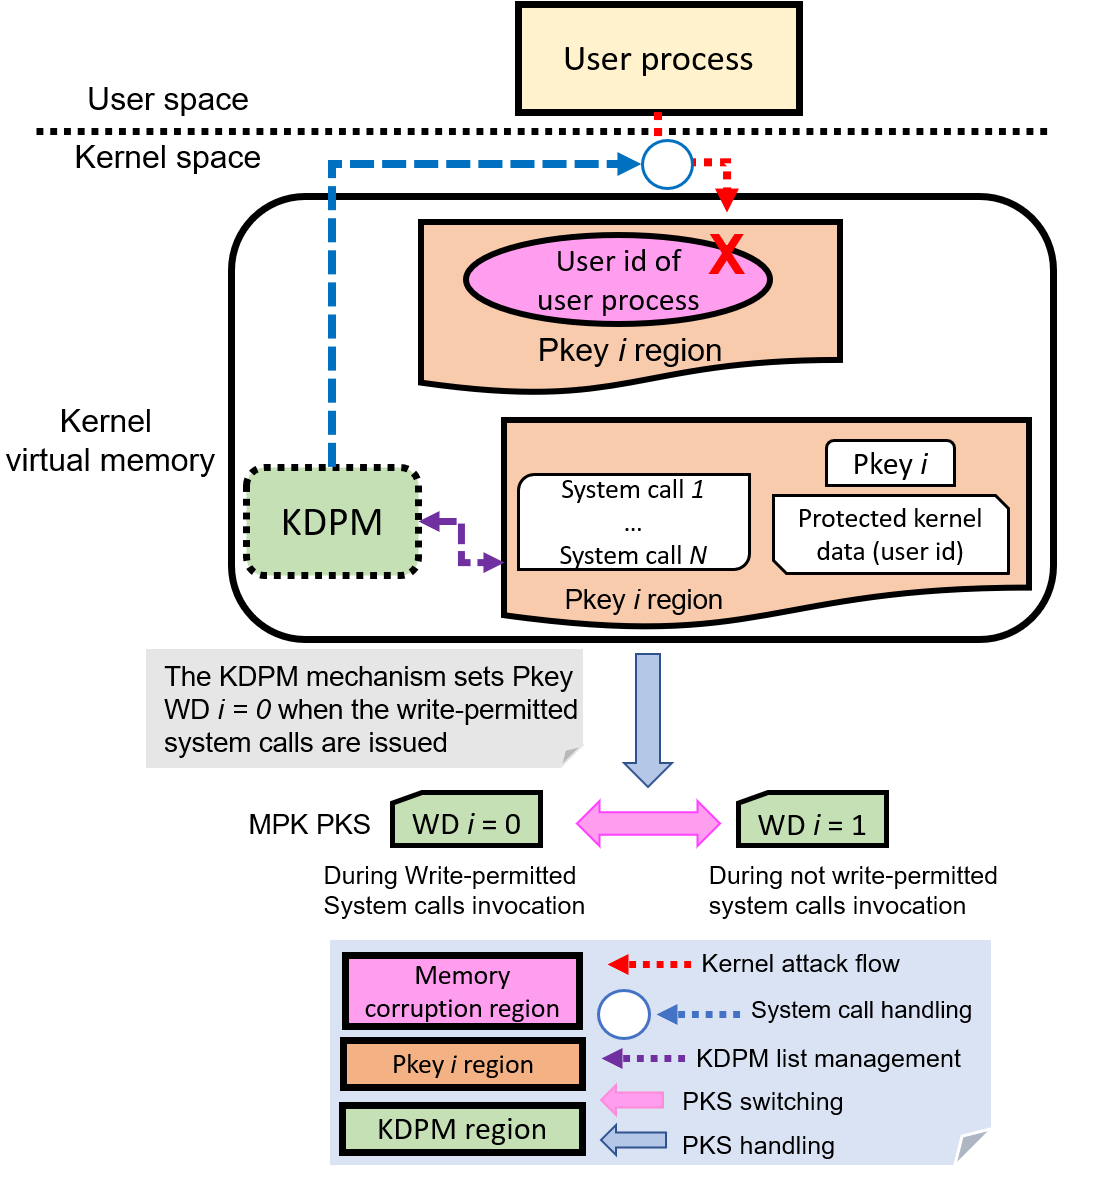
\includegraphics[bb=0 0 530 565, scale=.360]{./imgs/004_screenshot_2021-07-28_18.34.36.png}
  \end{center}
  % \vspace{-2.0ex}
  \caption{
    %
    % 提案するセキュリティ機構の実現方式1
    Implementation 1 of the KDPM
    %
  }
  % \vspace{-3.0ex}
 \label{fig:implementation1_overview}
\end{figure}

\begin{table}[t]
  \centering
    \caption{
      % 実現方式1における保護対象カーネルデータと書込み許可システムコール(参考文献 \cite{yamauchi21ijis} より抜粋)
      Protected kernel data and write-permitted system call of Implementation 1 
    }
\scalebox{1.00}{
%\hspace*{-5.0ex}  
\begin{tabular}{lc}
  %\hline
  \hline \noalign{\smallskip}
  \begin{tabular}{c}
    {\bf Item}
  \end{tabular}
  & 
  \begin{tabular}{c}  
  {\bf Description}
  \end{tabular}
  \\         
  \noalign{\smallskip}
  \hline
  \noalign{\smallskip}
  \multirow{2}{*}{Protected kernel data} & User ID (e.g., uid,euid,fsuid,suid)\\
                                         & Group ID (e.g., gid,egid,fsid,sgid)\\
  \multirow{2}{*}{Write-permitted system call}   & execve, setuid, setgid, setreuid, setregid\\
                                         & setresuid, setresgid, setfsuid, setfsgid\\         
  \hline
\end{tabular}
}
\label{tb:systemcall_list}
\end{table}


% \subsubsection{保護対象カーネルデータの書込み制御} \label{subsubsection:imp01_write_handling}
\subsubsection{Handling of Write Restrictions:} 

% 実現方式1において,書込み許可システムコールのリストに含めるシステムコールは,権
% 限情報の操作を行うシステムコールとし,\tabref{tb:systemcall_list}に示す.実現方
% 式1における, PKS Pkey を用いた保護対象カーネルデータの書込み制限の制御
% は,次の手順にて行う.
% The system calls to be included in the list of write permitted system calls in
% implementation method 1 shall be system calls that perform operations on
% authorization information. 

Implementation 1 admits the system calls that change the privileged
information (Figure \ref{tb:systemcall_list}). 
%
The process of controlling the write restrictions of the protected kernel data using Pkey is as follows:
% in implementation method 1 The following
% procedure is used.

% \begin{enumerate}[topsep=0pt]%\itemsep=-1.0ex \parskip=1.0ex  
\begin{enumerate}%[topsep=0pt]%\itemsep=-1.0ex \parskip=1.0ex  
%   \item ユーザプロセスによるシステムコール呼出しを捕捉.
\item The kernel identifies a system call invoked by a user process.
  
  
%   \item 書込み許可システムコールリストに含むシステムコール番号か判定.
\item The kernel determines if the system call number is included in the list of write-permitted system calls.

\begin{enumerate}%[topsep=0pt]%\itemsep=-1.0ex \parskip=1.0ex      
%   \item 書込み許可システムコールの場合:
%   PKSによる書込み制限制御を行い,保護対象カーネルデータを書込み許可に設定.
\item For write-permitted system calls: the kernel sets the protected kernel data with
the write-enable permission by the PKRS.
\end{enumerate}
  
% \item システムコールの実行を継続する.
% \item システムコールの終了後,
% PKSによる書込み制限制御を行い,保護対象カーネルデータを書込み制限に設定.
\item The execution of the system call is continued.
\item After the system call: the kernel restores the protected kernel data and
is set to the write-disable permission by the PKRS.
% writes restriction control 
% and 
% is performed

\end{enumerate}


% \subsection{実現方式2の個別処理}
\subsection{Implementation 2} \label{subsection:imp02_write_handling}

% 実現方式2の概要を図\ref{fig:implementation2_overview}に示す.実現方式2において
% は,書込み許可カーネルコードとして,セキュリティ機能の変更を伴うカーネルコード
% 実行時のみセキュリティ機能に関するカーネルデータの書込み制限を制御するため,
% LSMに関するカーネルデータの一覧,および書込み許可カーネルコードの一覧をリスト
% として管理する.
Figure \ref{fig:implementation2_overview} presents an overview of Implementation
2.
%
Implementation 2 adopts the write-permitted kernel code of the LSM and supports
the list of kernel data related to the LSM and that of the write-permitted
kernel codes.
% the kernel code for LSM is 
% In Scheme 2, the kernel code for LSM is the write-allowed kernel code.
%
Implementation 2 handles the write restrictions for the protected kernel data when
executing write-permitted kernel codes that change the access control policy and
access control decision.
%



% \subsubsection{保護対象カーネルデータ}
\subsubsection{Protected Kernel Data:}


\begin{figure}[t]
  \begin{center}
%    \hspace*{-5.0ex}
    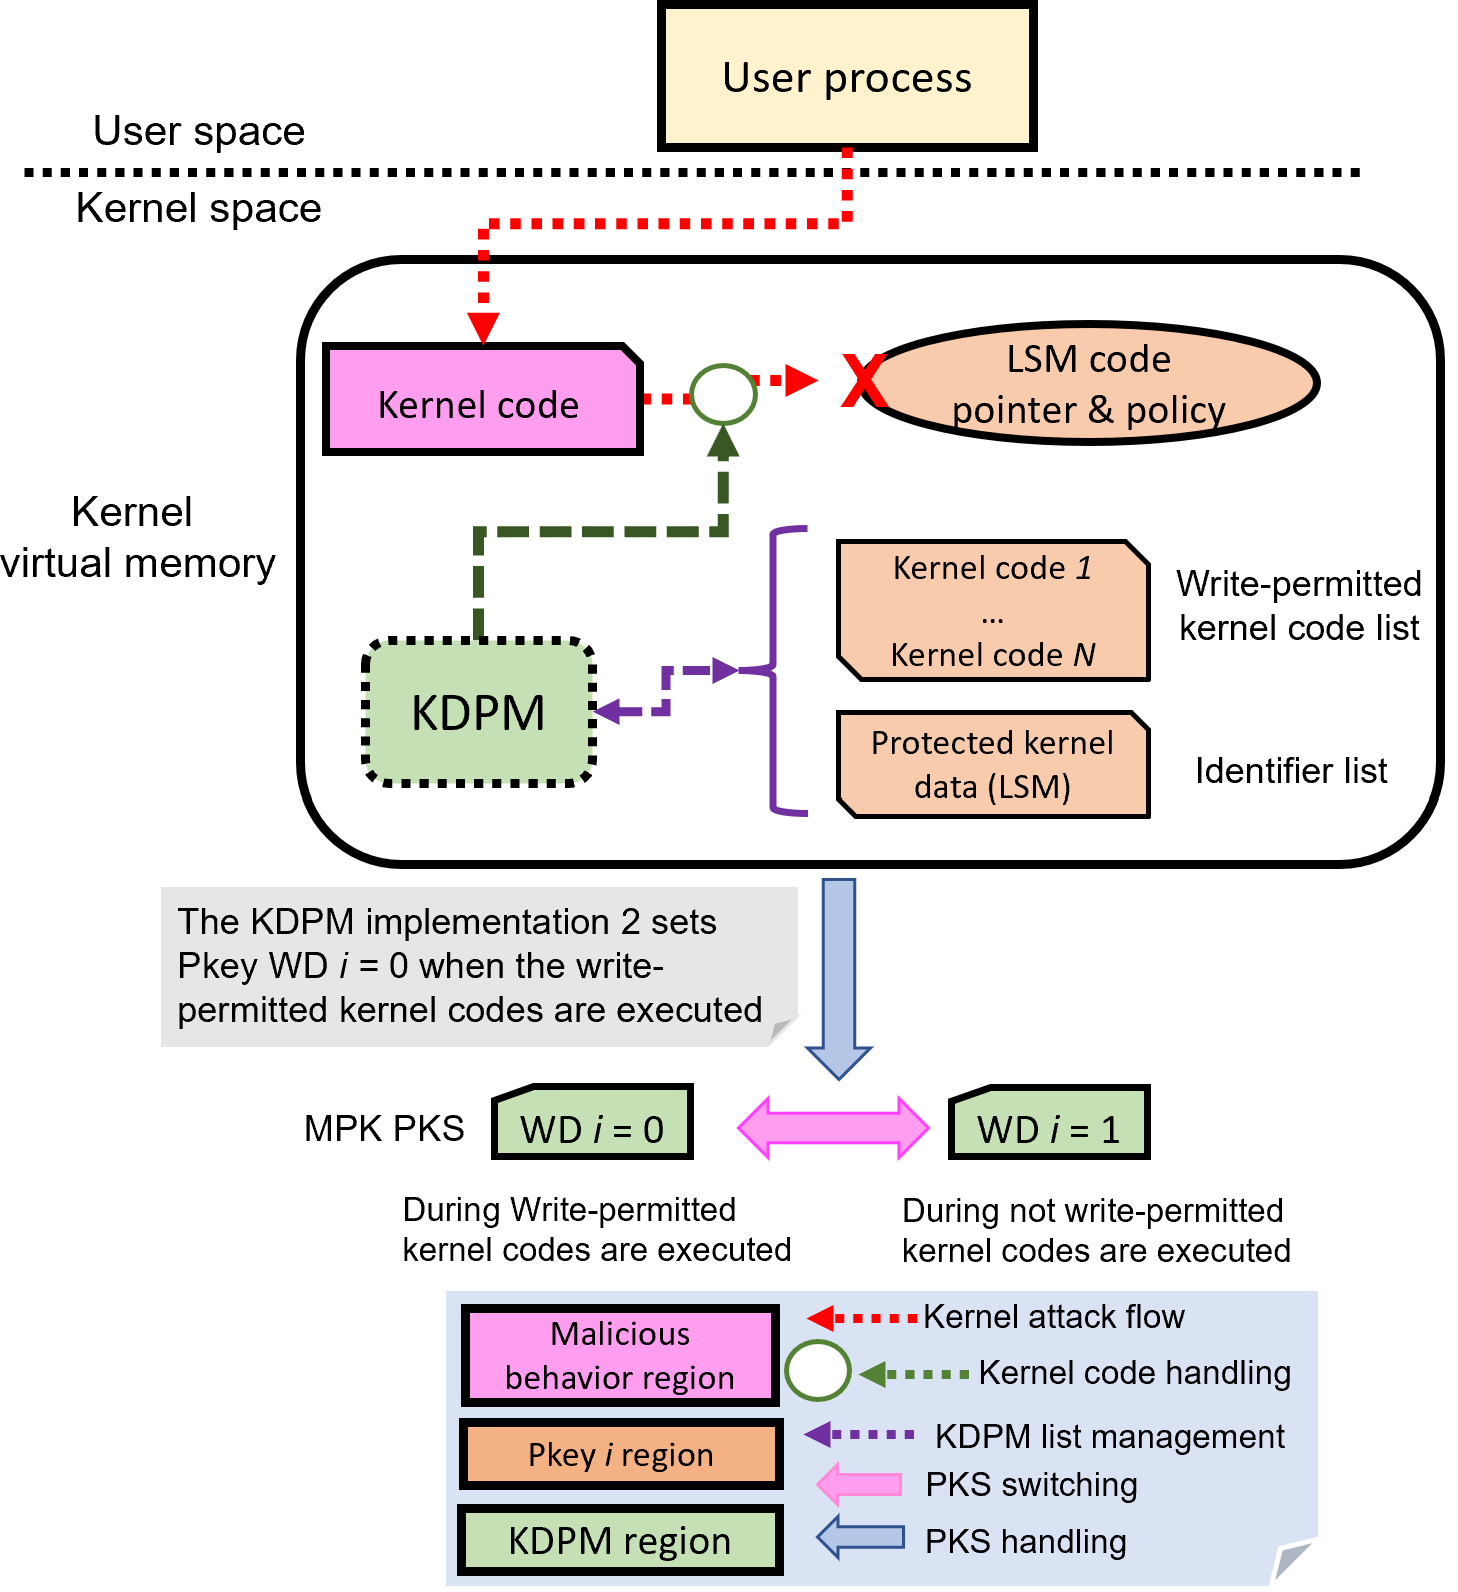
\includegraphics[bb=0 0 547 597, scale=.350]{./imgs/005_screen_shot_2022-01-10_180226.png}
  \end{center}
  % \vspace{-2.0ex}
  \caption{
    %
    % 提案するセキュリティ機構の実現方式2
    Implementation 2 of the KDPM
    %
  }
  % \vspace{-3.0ex}
 \label{fig:implementation2_overview}
\end{figure}


% 実現方式2において,保護対象とするカーネルデータは,\tabref{tb:kernel_code_list}
% に示すLSMに関連するカーネルデータの一部である関数ポインタを格納する変数,ならび
% にアクセス制御ポリシを格納する変数とるす.また,書込み許可カーネルコードのリスト
% についてもPKSを用いた書込み制限制御による保護対象とする.
Table \ref{tb:kernel_code_list} presents the kernel data to be protected in
Implementation 2. Additionally, \verb|selinux_hooks| is a variable that stores function
pointers that are part of the kernel data related to the LSM, and
\verb|selinux_state| is a variable that stores the access control policy. Furthermore,
the list of write-permitted kernel codes is protected by write restriction
control using the PKS.


\begin{table}[t]
  \centering
    \caption{
      % 実現方式2における保護対象カーネルデータと書込み許可カーネルコード.
      Protected kernel data and write-permitted kernel code of Implementation 2
    }
\scalebox{0.85}{
%\hspace*{-5.0ex}  
\begin{tabular}{lc}
  %\hline
  \hline \noalign{\smallskip}
  \begin{tabular}{c}
    {\bf Item}
  \end{tabular}
  & 
  \begin{tabular}{c}  
  {\bf Description}
  \end{tabular}
  \\         
  \noalign{\smallskip}
  \hline
  \noalign{\smallskip}
  \multirow{2}{*}{Protected kernel data} & Function pointer (e.g., selinux\_hooks)\\
                                         & Security policy (e.g., selinux\_state)\\
  \multirow{2}{*}{Write-permitted kernel code}   & Kernel functions in the selinux\_hooks\\
                                                 & avc\_init, avc\_insert, avc\_node\_delete, avc\_node\_replace\\         
  \hline
\end{tabular}
}
\label{tb:kernel_code_list}
\end{table}

% \subsubsection{保護対象カーネルデータの書込み制御} \label{subsubsection:imp02_write_handling}
\subsubsection{Handling of Write Restrictions:} 

% 実現方式2における保護対象カーネルデータのうち,LSMに関連するカーネルデータの関数
% ポインタを格納する変数,および書込み許可カーネルコード名リストは Linux カーネル
% の起動中に値が設定される.
% %
% 実現方式2においては,個々の値がカーネルデータに格納された直後にPKSによる書込み制
% 限対象とし,管理する.
% Among the kernel data to be protected in 
Implementation 2 stores the function pointer of the kernel data related to
the LSM, and the list of write-permitted kernel codes is set during the booting of the kernel.
% at the kernel booting.
%  to values during Linux kernel
% startup.
Table \ref{tb:kernel_code_list} also presents the kernel codes to be included in
the list of write-permitted kernel codes.

% In Implementation Scheme 2, each value is subject to write restriction by PKS
% immediately after it is stored in the kernel data, and is managed.

% %

% 実現方式2における書込み許可カーネルコードに対するPKSを用いた制限制御は次の手順にて行う.
The following procedure is used to control the restrictions on the write-permitted
kernel code using the PKS:
% in implementation method 2 

% %\begin{enumerate}
\begin{enumerate}[topsep=0pt]%\itemsep=-1.0ex \parskip=1.0ex  
%   %\item ユーザプロセスのコンテキストスイッチの発生を捕捉する.
%   \item 書込み許可カーネルコードにより,実現方式2のカーネルコードを呼出す.
\item The kernel invokes the kernel code of Implementation 2 during the execution of the write-permitted kernel code.
%  calls the kernel code of implementation method 2
  
%   %\item システムコール番号が権限変更許可リストに含まれるか判定.
%   \item 実現方式2のカーネルコードにて,書込み許可カーネルコードからの呼出しか判定.
\item The kernel code of Implementation 2 determines whether the caller belongs to a write-permitted kernel code.

% %  \begin{enumerate}
\begin{enumerate}[topsep=0pt]%\itemsep=-1.0ex \parskip=1.0ex      
%   \item 書込み許可カーネルコードの場合:PKSによる書込み制限制御を行い,保護対象カーネルデータを書込み許可に設定.
\item In the case of a write-permitted kernel code, the kernel performs write restriction control using the PKS to set the protected kernel data as write enabled.
%   \item 保護対象カーネルデータの書込み制限設定を検証するカーネルコードをタイマに登録,一定期間後に呼出すよう設定.
\item The kernel registers the write restriction of the protected kernel data in the timer and sets it to be called after a certain time.
% kernel code that verifies the write limit setting of the kernel data to be protected in the timer and set it to be called after a certain period of time.
      
\end{enumerate}
  
% \item 書込み許可カーネルコードの処理を継続.
\item The kernel continues processing the write-permitted kernel code.
% \item 書込み許可カーネルコードの終了前,実現方式2のカーネルコードを呼出し,
% PKSによる書込み制限制御を行い,保護対象カーネルデータを書込み制限に設定.
\item Before the end of the write-permitted kernel code, the kernel code of
Implementation 2 is called. The kernel performs write restriction using the PKS to set the
protected kernel data as write disabled.
% to be protected as write-limited.
% \item 書込み許可カーネルコードの処理を終了
\item The kernel finishes the processing of the write-permitted kernel code.

\end{enumerate}

% 書込み許可カーネルコードのリストに含めるカーネルコードは,
% \tabref{tb:kernel_code_list}のLSMの制御ポリシの操作を行うカーネルコードとする.

% 実現方式2において,タイマ登録される書込み制限設定を検証するカーネルコードでは,
% 書込み許可が意図せずに継続されることを防止する.
% %
% 書込み許可と制限を設定するカーネルコードの呼出し回数が一致しない場合,ならびに書
% 込み許可の継続時間が規定時間を超えた場合,強制的に書込み制限に設定する.
%
Implementation 2 verifies the write restriction setting using the timer to
prevent write as enable continued unintentionally.
% registered in 
%
% The implementation 2 is forced to set the write restriction.
% If 
Implementation 2 also checks the number of kernel code invocations to determine whether the
write restriction enabled and disabled are the same.
%
Further, Implementation 2 verifies whether the duration of write enable exceeds
the specified time.
%
% \reduline{ 
% The timer is a complementary feature to prevent missing of the configuration of
The timer is a complementary feature to prevent misconfiguration of
  the PKS protection setting. 
% to prevent the miss configuration of PKS protection setting. 
%
This timer usually requires sufficient time to miss it between starting and
finishing the execution of the write-permitted kernel code.
% execution start and finish.}
%  are not match, 


% \subsubsection{読書き制限の管理と操作}

% 実現方式において,権限情報 Protection key {\it i}に対する読書き制限
% RD{\it i},およびWD{\it i}は PKS の読書き制限操作レジスタ
% \verb|IA32_PKRS MSR|を用いて管理する.
% %
% %\verb|IA32_PKRS MSR|はCPUのコア単位に備えつけられており,権限変更許可
% \verb|IA32_PKRS MSR|はCPUコア毎に備えており,権限変更許可システムコー
% ル,および通常システムコール捕捉時の権限情報 Protection keyの読書き制
% 限の操作は,次の手順にて行う.

% %\begin{enumerate}
% \begin{enumerate}[topsep=0pt]\itemsep=-1.0ex \parskip=1.0ex  
%   \item ユーザプロセスによるシステムコール呼出しを捕捉.
  
%   \item 権限変更許可リストに含むシステムコール番号か判定.
  
% %  \begin{enumerate}
% \begin{enumerate}[topsep=0pt]\itemsep=-1.0ex \parskip=1.0ex      
%   \item 権限変更許可システムコールの場合:Protection key {\it i}に対応
%     する \verb|IA32_PKRS MSR| の RD{\it i},WD{\it i} に 0 を書込む
%     権限情報カーネルデータの読書き許可に設定
    
%   \item 通常システムコールの場合:Protection key {\it i}に対応する
%     \verb|IA32_PKRS MSR| の RD{\it i}に0を書込み,WD{\it i} に 1 を書
%     込む.権限情報カーネルデータの読込みのみ許可,書込みは不許可に設定.
%   \end{enumerate}
  
% \item システムコールの実行を継続する.
% \end{enumerate}


% 権限変更許可リストに含めるシステムコールは,
% \tabref{tb:privilege_data_list}の権限情報カーネルデータの操作を行うシ
% ステムコールとし,\tabref{tb:systemcall_list}に示す.


% \subsubsection{権限情報カーネルデータの保護事例}

% 実現方式を用いた権限情報カーネルデータの保護事例を
% \figref{fig:sample_case}に示す.
% %
% ユーザプロセスを起動後,権限情報 Protection key 1を権限情報カーネルデー
% タに設定する.
% %
% ユーザプロセスの発行したシステムコールが権限変更許可リストに含まれてい
% る場合,カーネルにおいてシステムコールの実行中,読書き制限操作レジスタ
% \verb|IA32_PKRS MSR| の RD1 および WD1 を 0 とし,権限情報の読書き操作
% を許可する.
% %
% 一方,システムコールが権限変更許可リストに含まれていない場合,システム
% コールの実行中,読書き制限操作レジスタ \verb|IA32_PKRS MSR| の RD1 は
% 0,WD1 は 1 とし,権限情報の書込みは許可されない.
% %

% \begin{figure}[tb]
%   \begin{center}
%     \hspace*{-5.0ex}
%     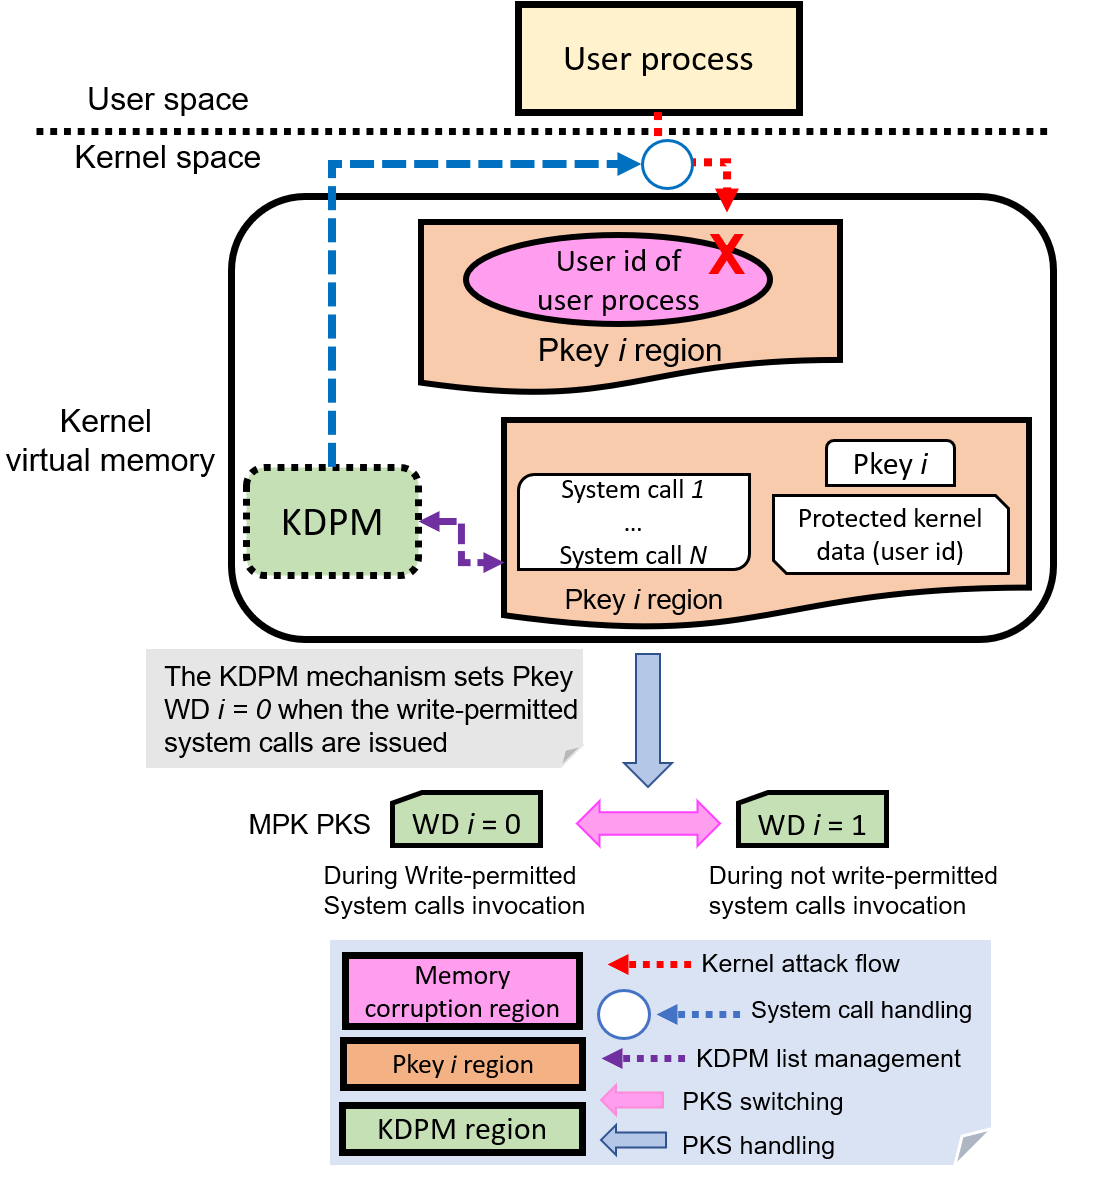
\includegraphics[bb=0 0 1033 887, scale=.265]{./imgs/004_screenshot_2021-07-28_18.34.36.png}
%   \end{center}
%   \vspace{-2.0ex}
%   \caption{
%     %
%     実現方式を適用した権限情報カーネルデータの保護
%     %
%   }
%   \vspace{-3.0ex}
%  \label{fig:sample_case}
% \end{figure}


%\subsubsection{プロファイル生成手順}
% \subsection{Profile Generation}
% vkTracer automatically generates a profile of the kernel vulnerability. 
% %
% Figure \ref{fig:approach_flow_overview} illustrates the steps of
% profile generation, which employs the trapping of the invocation of
% the kernel code and the identification of the virtual address ranges
% of the running kernel.
% This is achieved through the following steps:

% \begin{itemize}
% \item {\bf Step 1-1:}
%   The adversary executes the PoC code as a user process. vkTracer attaches to the adversary's user process and then registers the tracing target \verb|pid| for trapping.
  
% \item {\bf Step 1-2:}
%   The adversary's user process starts the kernel attack, which invokes the vulnerable kernel code by exploiting the kernel vulnerability.

% \item {\bf Step 1-3:} vkTracer determines whether the user process id
%   is the tracing target \verb|pid|, and then collects information on
%   the kernel code that is invoked by the adversary's user
%   process during each system call invocation.

% \item {\bf Step 1-4:}  vkTracer terminates the trapping of
%   the adversary's user process when the kernel is compromised through
%   the kernel vulnerability.

% \item {\bf Step 2-1:} vkTracer extracts the necessary kernel
%   information (e.g., invocation of kernel codes) from static and
%   dynamic kernel images to generate a profile of the kernel
%   vulnerability.


% \item {\bf Step 2-2A:} If the running kernel does not use KASLR, then vkTracer
%   creates a relationship among the kernel code, function name, and virtual
%   address ranges using the debug information of the kernel for the profile.

    
% \item {\bf Step 2-2B:} If the running kernel does use KASLR, then vkTracer
%   specifies whether the kernel image contains the kernel code as part
%   of the profile. The complement of the virtual address ranges is
%   identified for the profile at the kernel boot.
  
  
% \end{itemize}


% \subsection{Kernel Code Tracing}

% vkTracer uses the kernel tracing capabilities (e.g.,
% %
% \verb|bpftrace| and \verb|tracepoints|)
% %
% to associate the running kernel with the user process behavior.  The left
% side of Figure \ref{fig:tracing_implementation_overview} shows an
% overview of the tracing implementation and uses the following definitions.
% %% to attache the running kernel and user process behavior. The left side
% %% of Figure \ref{fig:tracing_implementation_overview} indicates the
% %% overview of tracing implementation.

% \begin{itemize}
% \item {\bf tracepoints}: This is a static embedded placement of a kernel that calls the tracing mechanism to record kernel processing.
%   %It is a static embedded placement of a kernel that calls the tracing mechanism
%   %to record the kernel processing.

% \item {\bf kprobes}:
%   This is a dynamically registered placement of a kernel that uses the symbol information of a function name for the kernel tracing capability.
  
%   %It is a dynamically registered placement of a kernel that
%   %uses the symbol information of a function name for kernel tracing capability.
%   %to calls an user defined enhanced Berkeley Packet Filter (eBPF) program 
% \end{itemize}

% The implementation of vkTracer employs the entire suite of kernel symbols and
% hooks the invocations of kernel code through \verb|kprobes|,
% %
% %The implementation of vkTracer employs the entire suite of kernel symbols and
% %hooks to the the invocations of kernel code thorough \verb|kprobes|.
% %
% whereas \verb|tracepoints| provides additional information about the kernel activity (i.e., system calls). 
% %
% %provides additional information of the kernel activity (i.e., system calls).
% %
% The implementation of vkTracer registers both tracing capabilities as
% a user-defined enhanced Berkeley Packet Filter (eBPF) program in the
% running kernel.
% %
% Therefore, vkTracer gathers the actual kernel code
% invocation history (e.g., function name list) from the target user
% process for the generation of the profile.

%% The implementation of vkTracer registers both tracing capabilities as user-defined enhanced Berkeley Packet Filter (eBPF) program into the running kernel.
%% %
%% Therefore, vkTracer gathers the actual kernel code invocation history (e.g., function name list) from the target user process for the generation of the profile. 
  


% \subsection{Virtual Address Range Identification}
% vkTracer analyzes the static and dynamic kernel images to identify the virtual
% address ranges for each kernel code for profile generation.
% %
% %vkTracer analyzes the static kernel image and the dynamic kernel image to identify the virtual address ranges for each kernel code for the profile generation.
% %
% Figure \ref{fig:tracing_implementation_overview} shows an overview of
% the virtual address identification implementation, which includes the following analyses:
% %indicates the overview of virtual address identification implementation.

% \begin{itemize}
% \item {\bf Static analysis of the kernel}:
%   %
%   vkTracer employs several sections of the Linux kernel. These are DWARF and
%   symbol information include \verb|.debug_info| and \verb|.text|, which contain
%   the kernel code and virtual address information.
  
%   %% vkTracer employs several sections of the
%   %% Linux kernel.  These are debug with attribute record format (DWARF)
%   %% is 
%   %% contains the kernel code and virtual address information.
% % \item 静的な仮想アドレス特定手段:KASLR有無に関わらず利用.カーネルの
%    %  DWARF情報として,カーネルデバッグに必要な情報として,\verb|.debug_info|
% %   \verb|.debug_info| セクションに格納されるDWARF(Debug With Attribute
% %     Record Format)情報,ならびにカーネルコードに関する \verb|.text|セク
% %   ションの情報を利用して仮想アドレス範囲を特定

% \item {\bf Dynamic analysis of the kernel}: vkTracer dynamically identifies the
%   virtual address range of the kernel code using the function name from
%   \verb|kprobes| and \verb|tracepoints| of the eBPF program.
%   %
%   Then, vkTracer prepares the Linux kernel module (LKM) that
%   requires the modified Linux kernel to employ \verb|EXPORT_SYMBOL| for
%   almost all kernel functions. It allows the LKM of vkTracer to
%   directly access the virtual address of the specified kernel function at
%   the kernel layer.
%   %vkTracer directory identifies the virtual address range of kernel code using the function name at the kernel layer.
% %}
% % \item 動的な仮想アドレス特定手段:KASLR有効時に利用,カーネルの起動時
% %   にカーネルコードを直接参照し,仮想アドレス範囲を特定
%  \end{itemize}

% The DWARF files contain multiple records of a program for debugging purposes.
% vkTracer parses the entirety of the records, and creates a relationship among
% the traced kernel code, virtual address range, and function name for the profile
% generation.
% %
% Table \ref{tb:dwarf_information} lists the DWARF information for the
% static analysis of the kernel. However, if the kernel uses
% KASLR, which performs a randomization of the virtual address range of
% the kernel code at each kernel boot, then vkTracer depends on a dynamic
% analysis of the kernel image to avoid infection from KASLR.


% \begin{table}[h]
%  \centering

% \caption{
% %
%   %  Portability consideration of MKM mechanism for OSes ($\checkmark$ is supported; $\triangle$ is partially supported).
%   DWARF information for profile ($\checkmark$ is adopted).
% %
% }
% %\vspace{-0.5ex}  
% \scalebox{1.00}{
% %  \begin{tabular}{c|cc}
% \begin{tabular}{llc}    
% %\hline
% \hline
% \noalign{\smallskip}
% %\begin{tabular}{c}
% %  {\bf Feature}
% %\end{tabular}
% \begin{tabular}{c}
%   {\bf Item}  
% \end{tabular}
% &
% \begin{tabular}{c}
%   {\bf Description}  
% \end{tabular}
% &
% \begin{tabular}{c}
%   {\bf Profile}
% \end{tabular}
% \\
% \noalign{\smallskip}
% \hline
% \noalign{\smallskip}
% DW\_AT\_name         & Function name                      & $\checkmark$ \\
% %DW\_AT\_decl\_file   & Function definition file name      & $\bullet$ \\
% %DW\_AT\_decl\_line   & Function definition line number    & $\bullet$ \\
% %DW\_AT\_type         & Return value type of function      & $\bullet$ \\
% DW\_AT\_low\_pc      & Lower virtual address of function  & $\checkmark$ \\ 
% DW\_AT\_high\_pc     & Higher virtual address of function & $\checkmark$ \\ 
% \hline
% \end{tabular}
% }
% \label{tb:dwarf_information}
% %\vspace{-1.0ex}  
% \end{table}



% \subsection{Termination Condition} \label{subsubsection:tracing_condition}

% vkTracer implements the following conditions for tracing completion:
% %  vkTracer implements the condition of tracing completion as following.  %}

% \begin{itemize}%\itemsep=-1.0ex \parskip=1.0ex

% \item {\bf Privilege escalation}: The adversary's user process
%   forcibly modifies its credential information (e.g., \verb|UID| is
%   \verb|0|) from normal privilege to administrator privilege.
% %  The adversary's user process forcibly modifies its credential
% %  information to the administrator privilege from the normal privilege.

% \item {\bf DoS}: The adversary's user process forcibly suspends the running
%   kernel after exploiting the kernel vulnerability. At this point, it will be
%   difficult to continue tracing the user process and kernel. Therefore, vkTracer
%   writes the history of the vulnerable kernel code's invocation to the disk
%   or sends these data to a remote server.

%   %% The adversary's user process forcibly suspend the running kernel
%   %% after the exploiting of kernel vulnerability.  It is difficult to
%   %% continue the tracing of user process and kernel, vkTracer writes the
%   %% history of vulnerable kernel code invocation to the disk or send
%   %% these to the remote server.

% \end{itemize}


% \subsection{Case Study}

% \subsubsection{User process tracing and kernel code identification}
% %\subsubsection{ユーザプロセスの追跡例}

% A case study was performed on the user process tracing and virtual address range
% for kernel code identification based on the profile of a specific kernel code
% (\verb|vfs_write|) using vkTracer.
% %
% As a demonstration of the tracing condition (in Section \ref{subsubsection:tracing_condition}),
% %
% Figure \ref{fig:tracing_sample_case} shows that the user process
% invokes a write system call and then switches its privilege from that
% of a user account to an administrator level.
% %
% vkTracer attaches to the user process, catches the invocation of
% the \verb|vfs_write| kernel code, and then finishes the tracing when
% the privilege of the user process becomes that of the administrator.
% % account.
% %
% Subsequently, vkTracer identifies the virtual address range of the
% \verb|vfs_write| kernel code, which is \verb|ffffffff811b8cd0| to
% \verb|ffffffff811b8e64| for the profile of \verb|vfs_write|.

% \begin{figure}[t]
%   \centering
%   \includegraphics[bb=0 0 541 457, scale=.275]{./imgs/A01X_04_screenshot_2021-05-26_4_38_28.png}

%     %  \vspace{-4.5ex}  
%   \caption{
%     %
%     Case study of tracing and kernel code identification
%     %
%   }
%   \label{fig:tracing_sample_case}
% %\vspace{-5.0ex}        
% \end{figure}



%% As case study of user process tracing and virtual address range of kernel code identification
%% as the profile of specific kernel code (e.g., \verb|vfs_write|) on vkTracer.
%% %
%% Figure \ref{fig:tracing_sample_case} shows that the user process invokes
%% %
%% \verb|write|
%% system call, then switches its privilege to administrator level from user account
%% for the demonstration of tracing condition (section \ref{subsubsection:tracing_condition}).
%% %
%% vkTracer attaches the user process and catches the invocation of 
%% %
%% \verb|vfs_write|
%% %
%% kernel code, then finishes the tracing when the privilege of the user
%% process becomes that of administrator account. After that, vkTracer
%% identifies the virtual address range of
%% %
%% \verb|vfs_write|
%% %
%% kernel code which is
%% %
%% \verb|ffffffff811b8cd0| to \verb|ffffffff811b8e64|
%% %
%% for the profile of \verb|vfs_write|.


%% \subsection{Restriction Implementation}


%% \blueuline{
%% The implementations of restriction of KPRM on a Linux kernel with x86\_64 CPU
%% architecture.
%% %
%% Linux with the restriction of KPRM manages the kernel page table that
%% controls the visible kernel pages for an adversary's user process.
%% }

%% Table \ref{tb:consideration_implementation} illustrates \blueuline{the
%% restriction of KPRM implementations, comparing their different
%% characteristics and effects.}
%% %
%% Figures \ref{fig:approach_implementation_1} shows that \blueuline{the restriction of
%% KPRM implementation 1 can prevent invocation of vulnerable kernel code and
%% protect kernel data.}
%% \blueuline{
%% It controls the references of restricted kernel pages on the additional
%% kernel address space of kernel page table for the adversary's user
%% process.}
%% %
%% Figure \ref{fig:approach_implementation_2} shows that \blueuline{the restriction of
%% KPRM implementation 2 can prevent kernel data memory corruption. It
%% requires complex handling for the references of restricted kernel pages
%% on the shared kernel address space of one kernel page table.}

%% \begin{table}[h]
%%  \centering

%% \caption{
%% %
%%     Implementations of KPRM ($\circ$ is covered; $\bullet$ is non-covered;).
%% %
%% }
%% %\vspace{-1.0ex}  
%% \scalebox{1.0}{
%% %  \begin{tabular}{c|cc}
%% \begin{tabular}{ccc}    
%% %\hline
%% \hline
%% %\noalign{\smallskip}
%% %\begin{tabular}{c}
%% %  {\bf Feature}
%% %\end{tabular}
%% {\bf Item}  & {\bf Implementation 1} & {\bf Implementation 2}\\
%% %\noalign{\smallskip}
%% \hline
%% %\noalign{\smallskip}
%% Kernel data protection         & $\circ$      & $\circ$  \\
%% Kernel code restriction         & $\circ$      & $\bullet$ \\
%% Stability effect                & Low          & High \\
%% Performance effect              & High         & Low \\
%% \hline
%% \end{tabular}
%% }
%% \label{tb:consideration_implementation}
%% %\vspace{-3.0ex}  
%% \end{table}


%% \begin{figure*}[t]
%%   \centering    
%%   \hspace*{-10.0ex}    
%%     \includegraphics[bb=0 0 1771 999, scale=.245]{./imgs/004_screen_shot_2019-08-04_12.55.50.png}
%% %  \vspace{-1.0ex}
%%   \caption{
%%     %
%%     Implementation 1 of kernel page restriction mechanism
%%     %
%%   }
  
%% %  \vspace{-1.0ex}  
%%   \label{fig:approach_implementation_1}
%% %  \vspace{-1.0ex}
%% \end{figure*}



%% \begin{figure*}[t]
%%   \centering    
%%   \hspace*{-10.0ex}    
%%     \includegraphics[bb=0 0 1770 996, scale=.245]{./imgs/005_screen_shot_2019-08-04_13.49.13.png}
%% %  \vspace{-1.0ex}
%%   \caption{
%%     %
%%     Implementation 2 of kernel page restriction mechanism
%%     %
%%   }
  
%%   %\vspace{-1.0ex}  
%%   \label{fig:approach_implementation_2}
%% %  \vspace{-1.0ex}
%% \end{figure*}
 

%% \subsubsection{Restricted Kernel Page Management}

%% Linux with \blueuline{both the implementations of the KPRM handle}
%% benign identification \verb|benign| flag on the struct
%% \verb|task_struct| to user process.
%% %
%% \blueuline{the restriction of KPRM} enables \verb|benign| flag to
%% refer application binary's absolute path within the benign user
%% process list \verb|benign_user_process_list|.
%% This list is manually created in the kernel source code.
%% \reduline{Additionally, the administrator modifies} \verb|benign|
%% \reduline{flag management via} \verb|/proc/pid/kprm|.
%% %
%% %Linux with KPRM
%% \blueuline{The restriction of KPRM} also manages the restricted kernel
%% page list \verb|restricted_page_list| that stores the restricted
%% kernel page information including \reduline{the list of kernel data
%%   and virtual address and the list of kernel code, the virtual
%%   address, and function name from profiles of kernel vulnerability.}
%% %
%% %A virtual address is related to the kernel code or kernel data.
%% %


%% \subsubsection{Implementation 1}
%% %
%% \blueuline{The restriction of KPRM implementation 1
%%   adopts an additional kernel page table with the Linux kernel page table
%%   structure.} 
%% %
%% Figures \ref{fig:approach_implementation_1} \blueuline{indicates that
%%   the implementation 1 of KPRM kernel creates the kernel address space
%%   of the page table for the kernel and it is restricted to system
%%   calls for the user process.}
%% %
%% The additional kernel page table is the variable \verb|kprm| of
%% \verb|mm_strct| on the struct \verb|task_struct|.

%% The additional kernel page table duplicates the initial value
%% \verb|pgd| of \verb|init_mm| to \verb|kprm| for the user process
%% creation.
%% %
%% During the running of the kernel, the KPRM kernel prepares
%% the PCID of TLB and then writes \verb|kprm| in \verb|current| to the
%% CR3 register for system call invocation.
%% %
%% KPRM also applies the timing of restricted kernel page handling.

%% The Linux kernel executes a task under the kernel address space
%% constructed from variable \verb|pgd| of \verb|current| when the kernel
%% receives an asynchronous interruption.
%% %
%% To overcome the issue of interruption, implementation 1 of KPRM kernel
%% switches to the kernel address space from the additional kernel
%% address space \verb|kprm| of \verb|current|.
%% %
%% This requires the writing of the CR3 register with the kernel page
%% tables as the variable \verb|pgd| of \verb|current| with PCID of TLB.


%% \subsubsection{Implementation 2}
%% \blueuline{The restriction of KPRM implementation 2
%%  adopts the directory management of the original kernel page table}
%% (Figures \ref{fig:approach_implementation_2}).
%% %
%% The KPRM kernel uses the variable \verb|pgd| of \verb|current| at the
%% system call invocation for the timing of restricted kernel page
%% handling.

%% The KPRM kernel directory modifies the original kernel page table,
%% which leads to unstable kernel behavior during interruption
%% processing.
%% %
%% For handling an interruption, implementation 2 of KPRM kernel affixes
%% the restricted kernel page references to the original kernel page
%% table \reduline{for kernel tasks exectuion.}

%% \subsubsection{Page Fault}
%% \blueuline{
%% During the user processoth on the Linux kernel with both implementations of KPRM,}
%% %the implementations of the KPRM
%% %Both the implementations of the KPRM
%% %
%% Linux kernels catch the page fault with the \verb|do_page_fault| or
%% the \verb|do_double_fault| function.
%% %
%% These functions indicate the virtual address of the cause of the page
%% fault.
%% %
%% \blueuline{
%%   Subsequently, the restriction of KPRM kernel inspects the detail of page fault that whether 
%%   virtual address is available for the user process.}
%% %
%% It further determines the access decision and maps the restricted
%% kernel page to the current kernel page table when the user process is
%% valid. Otherwise, it uses \verb|force_sig_info| to send SIGKILL to the
%% user process \blueuline{for the forcibly termination.}


%% \subsubsection{Restricted Kernel Page Handling}

%% \blueuline{
%%   The restricted kernel page handling is the common process for both
%%   implementations of KPRM.
%%   The KPRM kernel automatically adopts the hadling for the adversary's user process.
%% }
%% %
%% \blueuline{The handling timing is hardcoded into the KPRM kernel that
%%   adopts the handling steps before system call invocation in the}
%% %
%% \verb|entry_SYSCALL_64| function.

%% The handling mechanism identifies the page number from the virtual
%% address and subsequently unmaps the \reduline{reference of} restricted
%% kernel page from the target kernel page table with the
%% \verb|remove_pagetable| function.
%% %
%% The restricted kernel page is also unmapped from the direct
%% mapping region.
%% %
%% \blueuline{
%% Additionally, KPRM kernel manages the page fault and trap handling related to
%% a restricted kernel page.
%% }

%% Figure \ref{fig:approach_attack_case_01} shows the handling mechanism
%% for an adversary process.
%% %
%% The restricted kernel page handling process is described below.


%% \begin{figure*}[t]
%% %  \begin{center}
%%   \centering    
%%   \hspace*{-4.0ex}        
%%     \includegraphics[bb=0 0 1759 976, scale=.250]{./imgs/003X_screen_shot_2019-08-04_16.52.28.png}
%% %  \end{center}
%% %  \vspace{-1.0ex}
%%   \caption{
%%     %
%%     KPRM for the adversary's user process    
%%     %
%%   }
%% %  \vspace{-2.0ex}  
%%   \label{fig:approach_attack_case_01}
%% %  \vspace{-2.0ex}
%% \end{figure*}




%% %\vspace{-1.0ex}    
%% %\begin{itemize}\itemsep=-1.0ex \parskip=1.0ex
%% \begin{enumerate} %\itemsep=-1.0ex \parskip=1.0ex
%%   %
%% \item \reduline{vkTracer preprares the profiles of
%%   kernel vulnerability for the handling process (section \ref{subsection:tracing_implementation}).}
  
%%   \item KPRM \blueuline{kernel} creates and stores restricted kernel
%%     pages to the restricted kernel page list
%%     and the benign user process list at kernel booting.

%%     \begin{enumerate}
%%     \item  \reduline{KPRM kernel registers the virutal address of kernel codes
%%       into the restricted kernel page list from the profiles of kernel vulnerability.
%%       Additionally, KPRM kernel also registers the virtual address of kernel doata
%%       into the restricted kernel page list from the list of protected kernel data.}
%%     \end{enumerate}
    
%%     %
%%   \item An adversary's user process starts the system call execution,
%%     following which the KPRM kernel traps the system call routing and moves
%%     to KPRM kernel processing.
%%     %
%%   \item
%%     KPRM kernel determines adversary's user process identifies with
%%     \verb|benign| flag is off, and then KPRM kernel restores the restricted
%%     kernel pages from the restricted kernel page list and subsequently
%%     unmaps all of \blueuline{their references of kernel page} in the
%%     kernel page table.
%%     %
%%   \item
%%     The system call is invoked along with access to the kernel code of the system call routine,
%%     following which the kernel issues the page fault and KPRM kernel traps the page fault.
%%     %
%%   \item
%%     KPRM kernel identifies the virtual address of the page fault that
%%     indicates the virtual address of kernel code is on the restricted
%%     kernel page.
%%     \begin{enumerate}
%%     \item  In case of an invalid accesses of the restricted kernel page,
%%       KPRM kernel denies access from the user process.
%%         %
%%     \item If the access is valid, KPRM kernel maps the reference of
%%       restricted kernel page of the kernel code  to the kernel page table
%%       for the user process to continue.
%%     \end{enumerate}
%%     %
%%   \item    
%%     The system call routine's kernel code accesses kernel data; then,
%%     the kernel also issues the page fault, and KPRM kernel traps the page
%%     fault.
%%     %
%%   \item KPRM kernel identifies the virtual address of the page fault that indicates
%%     the virtual address of kernel data is on the restricted kernel page.
%%     %
%%     \begin{enumerate}      
%%     \item In case of an invalid access of kernel data on the
%%       restricted kernel page, KPRM kernel denies access from the user
%%       process.
%%         %
%%     \item If the access is valid, KPRM kernel maps the restricted kernel page of kernel data
%%       to the kernel page table for the user process to continue.
%%     \end{enumerate}        
%%   \item If KPRM kernel determines an adversary's process, access is not
%%     allowed on the restricted kernel page, and KPRM kernel sends a signal to
%%     the user process.
%% \end{enumerate}  
%% %\vspace{-1.0ex}



%% %{\bf Vulnerable Kernel Code Invocation and Memory Corruption:}
%% \subsubsection{Vulnerable Kernel Code Invocation and Memory Corruption}
%% %
%% \blueuline{
%%   As a case study of kernel memory corruption exploits kernel vulnerability,
%% }
%% Figure \ref{fig:approach_actual_attack_case_01} shows that
%% \blueuline{the adversary's user process employs}
%% CVE-2017-16995 \cite{CVE-2017-16995} PoC code invokes the vulnerable
%% kernel code at the eBPF system call.
%% %
%% The vulnerable kernel code is the \verb|map_update_elem| function of
%% \verb|kernel/bpf/syscall.c|.
%% %
%% \blueuline{
%%   The adversary's user process tries to invoke the vulnerable kernel code
%%   to modify the virtual address of the privilege information of kernel data
%%   on the kernel address space. After the success of privilege escalation, the
%%   adversary's user process executes the shell with administrator privileges.
%% }  

%% To prevent such attacks, implementation 1 of the KPRM kernel specifies
%% the vulnerable kernel code as \verb|map_update_elem| function to the
%% restricted kernel page. Then, the adversary's user process cannot
%% invoke the vulnerable kernel code. 
%% %
%% \blueuline{
%% Additionally, both implementations of the KPRM kernel specify kernel
%% data (e.g., privilege information) to the restricted kernel page. The
%% adversary's user process of the PoC code cannot modify the restricted
%% kernel page.}
%% %
%% Next, a page fault of the restricted kernel pages occurs.
%% %
%% Both the implementations of the KPRM kernel can catch this page fault to
%% determine whether to send SIGKILL to the attack process in the page
%% fault handler.

%% \begin{figure*}[t]
%% %  \begin{center}
%%   \centering    
%%   \hspace*{-2.0ex}        
%%     \includegraphics[bb=0 0 1770 964, scale=.260]{./imgs/006_screen_shot_2019-08-07_15.54.13.png}
%% %  \end{center}
%% %  \vspace{-1.0ex}
%%   \caption{
%%     %
%%     Handling of restricted kernel page reference for the actual kernel vulnerability
%%     %
%%   }
%% %  \vspace{-2.0ex}  
%%   \label{fig:approach_actual_attack_case_01}
%% %  \vspace{-2.0ex}
%% \end{figure*}

%\subsection{Tracing Implementation} \label{subsection:tracing_implementation}

%% 提案手法の実現環境は x86\_64 CPUアーキテクチャの Linux を想定し,特定
%% のユーザプロセスを指定した際にカーネルコード呼出しの追跡ならびにカーネ
%% ルコードと仮想アドレス範囲の特定を行う実現方式を考案した.
%
%, as follows:
%In this study, the implementation of vkTracer is implemented on Linux for the
%x86\_64 CPU architecture.
%% indicates the steps of profile
%% generation that employs the trapping of the invocation of kernel code
%% and the identification of the virtual address ranges of the running
%% kernel as following:
%% \begin{itemize}
%% \item 特権奪取:攻撃を行うユーザプロセスの実行前後において,権限情報の
%%   通常ユーザから特権ユーザへの変化を攻撃成功とみなす.

%% \item DoS:攻撃を行うユーザプロセスの実行中にカーネルが停止した場合,
%%   攻撃成功とみなす.カーネルが停止する場合,カーネルコードの呼出し履歴
%%   の取得が困難となることから,永続性のある記録媒体へのカーネルコードの
%%   呼出毎の保存,またはリモートの計算機へのログ出力を行う.

%% \end{itemize}

%\reduline{vkTracer finishes the trapping of the PoC
%  code as the user process, vkTracer starts to generate a
%  profile of kernel vulnerability from the necessary information of
%  tracing result.}% in \ref{subsection:attack_scenario}. }

% \begin{figure*}[t]
%   \centering
%   %\hspace*{-8.0ex}  
%   \includegraphics[bb=0 0 1103 608, scale=.390]{./imgs/A01X_03_screenshot_2021-05-26_5_25_02.png}
%       %  \vspace{-4.5ex}  
%   \caption{
%     %
%     Implementation of profile generation
%     %
%   }
%   \label{fig:tracing_implementation_overview}
% %\vspace{-5.0ex}        
% \end{figure*}



%  The adversary executes the PoC code as the user process. vkTracer
%  attaches the adversary's user process, then registers tracing target \verb|pid| for the trapping.


  %The adversary's user process starts the kernel attack that
  %invokes the vulnerable kernel code through exploiting the kernel vulnerability.

  %% vkTracer determines whether the user process id is
  %% the tracing target \verb|pid|, then collects the kernel code information which is
  %% invoked by the adversary's user process during each the system call invocation.

  %% vkTracer extracts the necessary
  %% kernel information (e.g., the invocation of kernel codes) from the
  %% static and dynamic kernel image to generate the profile of kernel
  %% vulnerability.

  % KASLR randomized the virtual address ranges of the kernel code for each kernel boot. 
  
  %% vkTracer creates the relationship between the kernel code ,
  %% function name, and virtual address ranges using the debug information
  %% of the kernel for the profile when the running kernel does not adopt
  %% KASLR that randomizes virtual address ranges of kernel code for each
  %% kernel boot.
  
  %% If the running kernel adopts KASLR, vkTracer specifies
  %% that whether the kernel image contains the kernel code as the part of
  %% profile. The complement of virtual address ranges is identified for
  %% the profile at the kernel boot.
  
  %that KASLR randomizes virtual address range of kernel code for each kernel boot.%% The dwarf information contains multiple records of a program for debugging purposes. vkTracer parses the whole of records, then makes the relationship between the traced kernel code, virtual address range, function name for the profile generation.
%% %
%% Table \ref{tb:dwarf_information} shows the list of dwarf information
%% for static analysis of the kernel.
%% %  
%% In addition, due to the randomization of the virtual address range of kernel code at each KASLR enable kernel boot, vkTracer depends on the dynamic analysis of the kernel image to avoid the infection of KASLR.

%% 実現方式において,追跡対象のユーザプロセスを動作させ取得したカーネル関
%% 数名一覧から仮想アドレス範囲の特定は,以下の静的な仮想アドレス特定手段
%% ならびに動的な仮想アドレス特定手段により行う.両方の手段を利用するかは
%% カーネルの仮想空間におけるカーネルコードの位置を起動毎に変化させる
%% KASLRの有無に依存する.

%% \begin{itemize}
%% \item 静的な仮想アドレス特定手段:KASLR有無に関わらず利用.カーネルの
%%   %  DWARF情報として,カーネルデバッグに必要な情報として,\verb|.debug_info|
%%   \verb|.debug_info| セクションに格納されるDWARF(Debug With Attribute
%%     Record Format)情報,ならびにカーネルコードに関する \verb|.text|セク
%%   ションの情報を利用して仮想アドレス範囲を特定
  
%% \item 動的な仮想アドレス特定手段:KASLR有効時に利用,カーネルの起動時
%%   にカーネルコードを直接参照し,仮想アドレス範囲を特定
%% \end{itemize}

%% 静的な仮想アドレス特定手段にて用いるDWARF情報の値を表
%% \ref{tb:dwarf_information}に示す.DWARF情報を利用することで,仮想アド
%% レス範囲,定義ファイル,定義位置,関数の型,引数の数,ならびに引数の型
%% 等を特定することが可能である.

%% 追跡対象のユーザプロセスを実行した際,\ref{subsection:design} 節で示し
%% た一連の処理により,カーネルにおいてユーザプロセスから呼び出されたカー
%% ネルコードが列挙され,最終的にカーネルコードに対応する仮想アドレス範囲
%% の一覧が得られる.カーネルへの攻撃に紐づくカーネルコードかの判断は,カー
%% ネル脆弱性を利用した攻撃の成功可否を判定して行う.
%% %攻撃の成功可否を判定することが必要である.
%\reduline{
%
%  when
%the user process completes the attacking scenario (in section
%\ref{subsection:attack_scenario}) 
%% 提案手法においては,カーネル脆弱性を介して攻撃可能なPoC コードを実行す
%% る際に,以下のカーネル脆弱性毎の攻撃成功可否基準に従い,攻撃の有効性を
%% 判定する.
%% %攻撃成功時には基づいてカーネル脆弱性および関連するカーネルコードを特定する.

%% %,カーネルコードの推測が可能だと考えているが,CVE,PoCコー
%% %ド,ならびにカーネルのソースコード修正履歴を参照しながら特定する必要が
%% %ある.


% # -*- coding: utf-8 -*-
\section{Evaluation} \label{seciton:evaluation}
\subsection{Security Capability}

% 評価として,提案するセキュリティ機構を適用したカーネルにおいて,特権奪取攻撃か
% ら権限情報保護が適切に動作するかの調査を目的とする.セキュリティ機能評価の項目
% と内容を以下に示す.
The security capability evaluation validates whether the kernel with the
KDPM adequately protects privileged information.
% properly protect privilege information.
% from privilege-grabbing attacks. The items and contents of the security function
% evaluation are listed below.

% %\begin{enumerate}%[leftmargin=1.0cm,topsep=0pt ]\itemsep=-1.0ex \parskip=1.0ex
\begin{enumerate}%[topsep=0pt]%\itemsep=-1.0ex \parskip=1.0ex  

% \item 特権奪取攻撃に対するセキュリティ機能の評価
\item Prevention of privilege escalation attack\\
%   提案するセキュリティ機構を適用したカーネルに対して,特権奪取攻撃に利用可能な
%   カーネル脆弱性を導入し,特権奪取攻撃を行うユーザプロセスを実行する.
%   %
%   予め権限情報Protection keyの書込み制限を有効化,特権奪取攻撃実行時に,権限情
%   報の改ざん防止を実現可能か評価した.
%
% A kernel vulnerability that can be used for a privilege escalation attack is
% introduced into the kernel with the proposed security mechanism applied, and a
% user process that performs a privilege escalation attack is executed.
%
A kernel vulnerability that can be exploited for a privilege escalation attack is
introduced into the Linux kernel.
%
We evaluate the kernel with Implementation 1, which enables the write
restriction of the privileged information of user processes. This prevents an adversary
from performing a privilege escalation attack.
% to prevent an adversary's
% user process, which performs a privilege escalation attack. 

\item Preventing the defeat of security mechanism\\
We evaluate the kernel with Implementation 2, which enables the write
restriction of kernel data of the LSM to prevent MAC defeat.%the defeat of MAC. 


% We evaluated the security capability of the kernel with the proposed security mechanism
% preventing the falsification of authorization
% information by enabling the writing restriction of authorization information
% protection keys in advance, and by preventing the falsification of authorization
% information when a privilege-grabbing attack is executed.
\end{enumerate}

\subsection{Performance Evaluation}

% 提案するセキュリティ機構を適用したカーネルのセキュリティ機能評価は先行研究におい
% て示している\cite{kzn21css}.本稿では,

% 性能評価として,実現方式1に対して,ベンチマーク測定によるカーネルとユーザプロ
% セスへの動作影響有無の調査,および実現方式2で用いるPKS操作による性能への影響を
% 確認した.評価項目と内容を以下に示す.

In performance evaluation, we investigate whether the kernel and user processes
are affected by Implementation 1 and the effect of the PKS operations used in
Implementation 2.
% both
% in implementation 2.

% we investigated whether or not the kernel and user
% processes were affected by benchmark measurements for implementation method 1,
% and confirmed the effect of PKS operations used in implementation method 2 on
% performance. The evaluation items and their contents are listed below.

\begin{enumerate}%[topsep=0pt]%\itemsep=-1.0ex \parskip=1.0ex

% \item カーネル処理におけるオーバヘッド\\
\item Measurement of the kernel performance overhead\\
%     %
%     実現方式1を適用した Linux カーネルにおいて,ベンチマークソフトウェアを用いたシ
%     ステムコールのオーバヘッドの測定した.
To measure the performance of the Linux kernel with Implementation 1, the benchmark
software calculates the overhead of the system call invocation latency.

%   \item PKS操作におけるオーバヘッド\\
\item Measurement of PKS performance overhead\\
%     %
%     提案するセキュリティ機構で用いる PKS の利用にかかるオーバヘッドとして,PKS 操
%     作に関する処理時間を測定した.
To measure the performance of the PKS in the KDPM, we measure the processing
time of the PKS operations in the Linux kernel with Implementation 2.
%Specifically, we measured the processing time of PKS operations in the Linux kernel.
% We measured the overhead of using PKS in the proposed security mechanism.
% Specifically, we measured the processing time related to PKS operations.

\item Measurement of the kernel instruction increasing\\
To measure the instruction insertion of the Linux kernel with Implementations,
the disassembling tool indicates the additional instructions. 

\end{enumerate}
  

% \subsection{Tracing and Identification Capability}
% %\reduline{
% The ability of vkTracer to identify vulnerable kernel code information, when an
% adversary's user process attempts to exploit a proven kernel vulnerability in
% invoking a system call, was evaluated.
% %
% The assessment of vkTracer was validated by identifying the vulnerable kernel
% code. 



% \subsection{Performance Measurement}
% To evaluate the performance costs of tracing, identification, kernel, and 
% user process overhead were measured.

% \begin{enumerate}%[leftmargin=0.5cm]%\itemsep=-1.0ex \parskip=1.0ex
% \item {\bf Measurement of vulnerable kernel code identification}:
%   %
% %  \reduline{
%     Tracing and identification cost was measured using the PoC
%     applications.
    
% \item {\bf Measurement of the kernel overhead}:
%   To measure the feasibility of tracing for the kernel, LMbench was %and sysbench were
%   used to calculate the overhead of the system call invocation latency.
%   %and system latency.

% \item {\bf Measurement of the application overhead}:
%   The application overhead for the web server and client was measured using nginx and ApacheBench.
    
% \end{enumerate}


\subsection{Evaluation Environment}

\subsubsection{Equipment:}
% PKSに対応したCPUは2022年1月時点では提供されていない.評価には CPU Intel(R)
% Core(TM) i7-7700HQ(2.80GHz,4コア),Memory 16 GBytes を備えた計算機を用い,性
% 能評価を行う仮想計算機環境として PKS に対応したQEMU 6.0.91を用いた \cite{qemu}.
% %
% QEMU上のゲストOSは Debian 10.2 とし,実現方式1を Linux kernel 5.3.18 を対象
% に,15個のファイルに対して431行を追加し実装した.また,PKS操作の性能負荷評価のた
% めの専用の測定プログラムとして165行を Linux カーネル に追加した.


%  containing one environment server and a log collection
% server.
%
%The environment for the evaluation of the performance cost was
% The environment for the PoC code, kernel, and web server for measuring
% The environment for the PoC code, kernel for 
% measuring the performance cost was implemented 
% The evaluation environment for 
We evaluated the PoC code and kernel using a physical machine equipped with an
Intel (R) Core (TM) i7-7700HQ (2.80 GHz, x86\_64) processor with 16 GB memory.
%
% The web client machine was equipped with an Intel (R) Core (TM)
% i5-4200U (1.6 GHz) processor with 8 GB of memory, running on Windows 10.
%

The security capability evaluation was implemented on a virtual machine because
QEMU 6.0.91 supports the PKS. However, the PKS is not available as of January
2022 on the Intel CPU.
%
The guest OS on QEMU was Debian 10.2, and Implementations required 15 source
files and 431 lines for Linux kernel 5.3.18.
%
% In addition, 
% The performance evaluation of the PKS operation require the measurement program
The PKS performance for Implementation 2 was evaluated using a
measurement program that required 165 lines for Linux kernel 5.3.18.
% for the purpose of measuring the performance of the system
% was added to the Linux kernel, 

%% \reduline{
% The network environment for the application benchmark was a 1
% Gbps hub supporting direct connections between the server and client
% machines.

% \subsubsection{特権奪取攻撃に利用可能なカーネル脆弱性}

\subsubsection{Implementation:}
%
%\reduline{
% vkTracer was implemented on the Linux x86\_64 CPU kernel.
%
To evaluate the security capability, a kernel vulnerability was introduced into
% the Linux kernel using a PoC code \cite{CVE-2017-6074} that leads to privilege
the Linux kernel using a PoC code \cite{CVE-2017-16995} that leads to privilege
escalation via memory corruption through the system call number 350.
%
% One kernel vulnerability 
Additionally, the Linux kernel module (LKM) attempted to overwrite the LSM function pointer to
defeat the MAC on the running kernel:
% which can be used for privilege escalation attacks 

\begin{itemize}%[topsep=0pt]
  
  %\item {\bf Memory Corruption}: The vulnerable kernel code 1 is
\item {\bf Privilege escalation:} Vulnerable kernel code 1 refers to
  CVE-2017-16995 \cite{CVE-2017-16995}, which was implemented as a system call
  \verb|sys_kvuln01|.
  %, \verb|support_sys_kvuln01_01|, and \verb|support_sys_kvuln01_02|.
  %
  The PoC code exploits the vulnerable kernel code to overwrite the privileged
  information of a user process for privilege escalation.

  \item {\bf Defeating security mechanism:} A customized LKM attempts to overwrite
  the function pointer of the kernel code that manages the LSM file access
  permission to circumvent the MAC decision.

\end{itemize}

% 提案するセキュリティ機構のセキュリティ機能評価のため,特権奪取攻撃に利
% 用可能な独自システムコールをシステムコール番号350としてカーネルに導入
% した.

% \vspace{-2.0ex}
% \begin{itemize}\topsep=-1.0ex \itemsep=-1.0ex \parskip=1.0ex  
  
% \item カーネル脆弱性(特権奪取):独自システムコールを実行中,権限
%   情報を変更するカーネル関数を呼出し,ユーザプロセスの権限情報を管理者
%   ユーザに変更する.

% \end{itemize}
% \vspace{-2.0ex}

% 評価において,独自システムコールを呼出すPoCコードをユーザプロセス経由
% にて実行し,特権奪取攻撃を行い,一般ユーザから管理者ユーザへの変更を
% 試みる.

% \subsubsection{特権奪取攻撃を行う独自システムコールの捕捉}
\subsection{Security Capability Evaluation Result}
\subsubsection{Prevention of Privilege Escalation Attack:}
% 攻撃を行うユーザプロセスによる独自のシステムコール捕捉時の動作結果を
% \figref{fig:kvuln1_1_04}に示す.
% of the operation when an original system call
The security evaluation result for the adversary's user process is shown in
Figure \ref{fig:kvuln1_1_04}.
% %
% \figref{fig:kvuln1_1_04} の3行目にて,プロセスID 1661の独自システムコール(シ
% ステムコール番号 350)の呼出しを捕捉している.5行目,および6行目にて,PKRS は
% 0x8 であり,Protection key 1 の書込み制限(WD1)は有効化されている.
In line 3, the kernel captures the original system call (i.e., system call
number 350) with process ID 1661. The kernel indicates 0x8, which indicates that
the write disable (WD) of Pkey 1 is enabled.
% %
% 10行目において,Protection key 1 の権限情報を格納するページへの書込みが行われ
% た際,ページフォルト(エラー番号 35)を捕捉している.捕捉されたページフォルト
% は Protection key により保護されたページへの書込み保護違反を示している.
In line 10, the kernel catches a page fault (i.e., error number 35) when writing
to the page that stores the privileged information with Pkey 1. The page fault
indicates a write protection violation of a page protected by the Pkey. In line
14, the kernel sends \verb|SIGKILL| to the user process of the adversary.

%
% 評価においては,特権奪取攻撃の動作確認のため,14行目から15行目にかけて,
% ページフォルト捕捉後,PKRS に 0x0 を書込み,Protection key 1 への書込
% み制限(WD1)を無効化し,特権奪取が成功することを確認している.
% In the evaluation, %we confirmed the operation of the privilege escalation attack,

% From the evaluation result, we confirmed that Linux kernel with the proposed
% security mechanism prevents privilege escalation attacks. The proposed mechanism
% can correctly handle the management of the Pkey and detect the memory
% corruption of a vulnerable kernel code.
% 1 after the page fault is caught, from line 14 to 15.

% writing 0x0 to PKRS and disabling the write restriction (WD1) to Protection key
% 1 after the page fault is caught, from line 14 to 15.

% \subsubsection{Prevention of Defeating Security Mechanism:}
\subsubsection{Preventing the Defeat of Security Mechanism:}
% 攻撃を行うユーザプロセスによる独自のシステムコール捕捉時の動作結果を
% \figref{fig:kvuln1_1_04}に示す.
% of the operation when an original system call
The security evaluation result of the LKM is shown in Figure
\ref{fig:defeat_mac}.
% %
% \figref{fig:kvuln1_1_04} の3行目にて,プロセスID 1661の独自システムコール(シ
% ステムコール番号 350)の呼出しを捕捉している.5行目,および6行目にて,PKRS は
% 0x8 であり,Protection key 1 の書込み制限(WD1)は有効化されている.
In line 2, the LKM attempts to find one of the function pointers of
\verb|selinux_hooks|. In line 5, LKM attempts to overwrite the function pointer of
\verb|selinux_hooks|.
% the kernel captured the original system call (i.e., system call
% number 350) with process ID 1661. The kernel indicates 0x8, which indicates that
% the write disable (WD) of Pkey 1 is enabled.
% %
% 10行目において,Protection key 1 の権限情報を格納するページへの書込みが行われ
% た際,ページフォルト(エラー番号 35)を捕捉している.捕捉されたページフォルト
% は Protection key により保護されたページへの書込み保護違反を示している.
In line 7, the kernel catches a page fault (i.e., error number 35) when writing
to the page storing the function pointer with Pkey 1. The page fault
indicates a write protection violation of a page protected by Pkey.
% In line 14, the kernel sends \verb|SIGKILL| to the user process of the adversary.

%
% 評価においては,特権奪取攻撃の動作確認のため,14行目から15行目にかけて,
% ページフォルト捕捉後,PKRS に 0x0 を書込み,Protection key 1 への書込
% み制限(WD1)を無効化し,特権奪取が成功することを確認している.
% In the evaluation, %we confirmed the operation of the privilege escalation attack,

From the security evaluation results, we confirmed that the Linux kernel with the
KDPM prevents privilege escalation attacks and avoids the defeat of security mechanism.
The KDPM correctly manages the Pkey and detect
memory corruption of the vulnerable kernel code.

% \begin{figure}[t]
%   \begin{center}
%   \hspace*{-8.5ex}    
%     \begin{tabular}{cc}

%       \begin{minipage}[t]{0.67\hsize}
%         % \begin{figure}[tb]
%         \begin{center}
%         % \hspace*{-09.0ex}
%           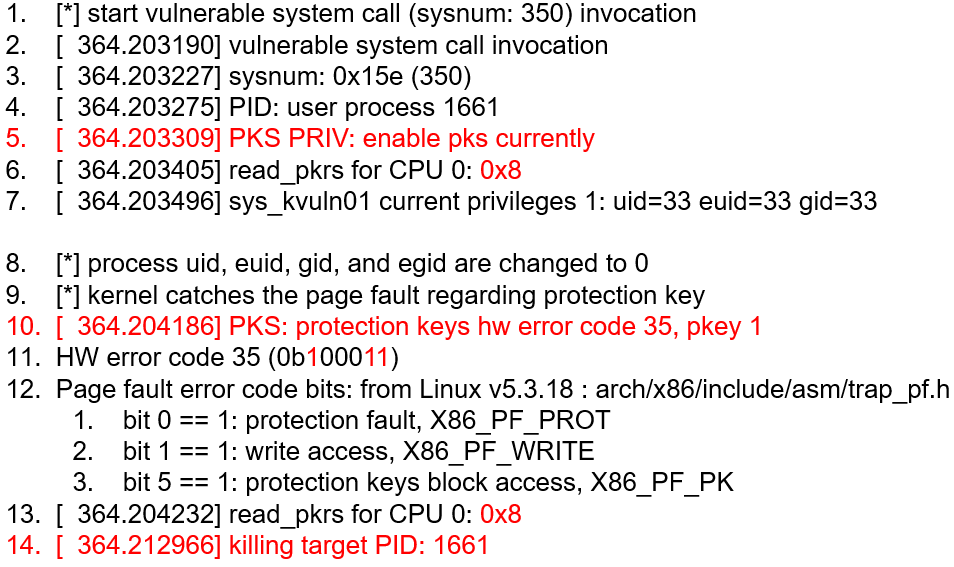
\includegraphics[bb=0 0 716 425, scale=.325]{./imgs/008_screenshot_2021-08-18_3.35.12.png}
%         \end{center}
%         % \vspace{-2.0ex}
%         \caption{
%         %
%         % 特権奪取攻撃に利用可能なシステムコール捕捉時の動作結果
%         Attack prevention of privilege escalation
%         %実現方式を適用した権限情報カーネルデータの保護
%         %
%         }
%         % \vspace{-4.5ex}
%         \label{fig:kvuln1_1_04}
%         %\end{figure}
%       \end{minipage} &

%       \begin{minipage}[t]{0.67\hsize}
%         \begin{center}
%         %\hspace*{-09.0ex}
%           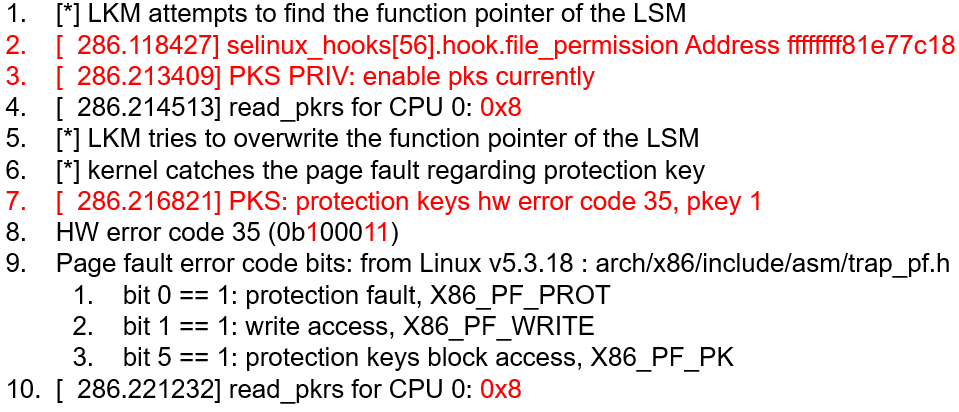
\includegraphics[bb=0 0 719 309, scale=.325]{./imgs/009_screenshot_2021-08-18_3.35.12.png}
%         \end{center}
%         % \vspace{-2.0ex}
%         \caption{
%         %
%         % 特権奪取攻撃に利用可能なシステムコール捕捉時の動作結果
%         Attack prevention of defeating MAC
%         %実現方式を適用した権限情報カーネルデータの保護
%         %
%         }
%         % \vspace{-4.5ex}
%         \label{fig:defeat_mac}
%         %\end{figure}
%       \end{minipage}
%     \end{tabular}
%   \end{center}
% \end{figure}

\begin{figure}[t]
  \begin{center}
    % \hspace*{-09.0ex}
      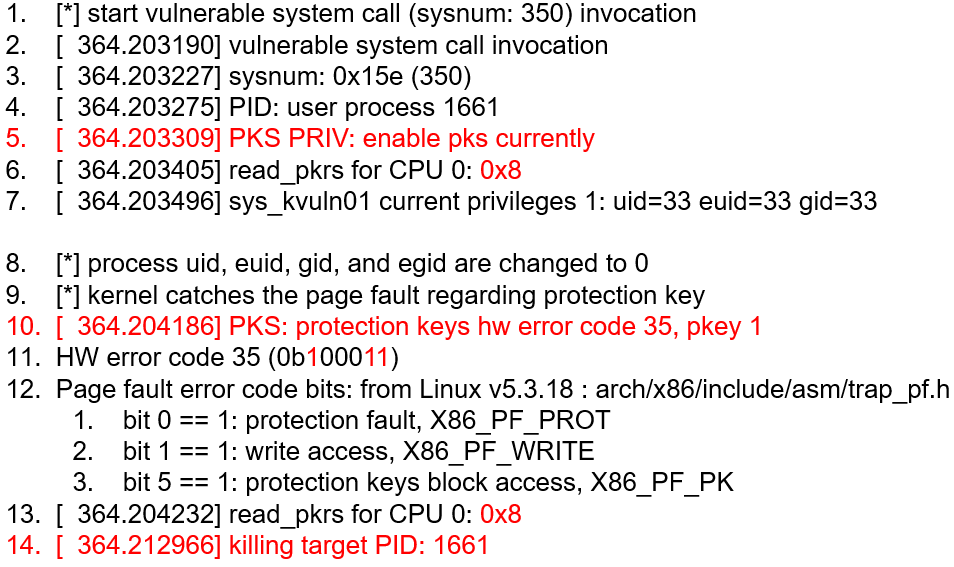
\includegraphics[bb=0 0 716 425, scale=.325]{./imgs/008_screenshot_2021-08-18_3.35.12.png}
    \end{center}
    % \vspace{-4.0ex}
    \caption{
    %
    % 特権奪取攻撃に利用可能なシステムコール捕捉時の動作結果
    Prevention of a privilege escalation attack
    %実現方式を適用した権限情報カーネルデータの保護
    %
    }
    % \vspace{-2.0ex}
    \label{fig:kvuln1_1_04}
\end{figure}

\begin{figure}[t]
  \begin{center}
    %\hspace*{-09.0ex}
      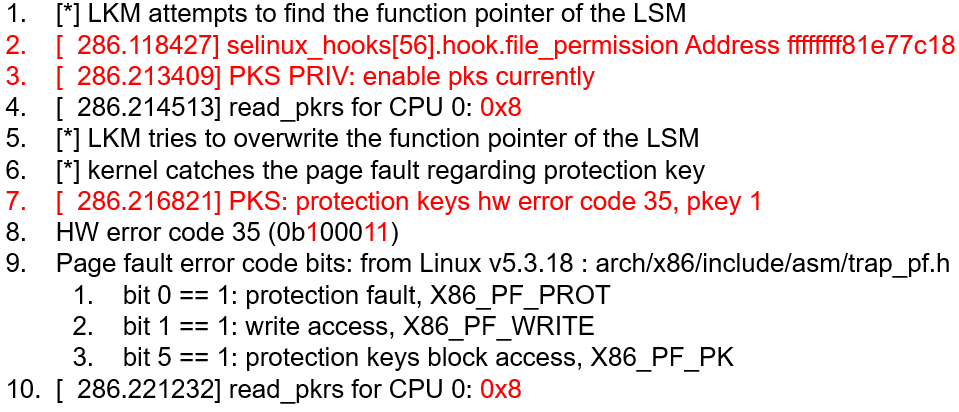
\includegraphics[bb=0 0 719 309, scale=.325]{./imgs/009_screenshot_2021-08-18_3.35.12.png}
    \end{center}
    % \vspace{-4.0ex}
    \caption{
    %
    % 特権奪取攻撃に利用可能なシステムコール捕捉時の動作結果
    Prevention of a MAC defeat
    %実現方式を適用した権限情報カーネルデータの保護
    %
    }
    % \vspace{-2.0ex}
    \label{fig:defeat_mac}
\end{figure}

% \begin{figure}[tb]
%   \begin{center}
% %    \hspace*{-09.0ex}
%     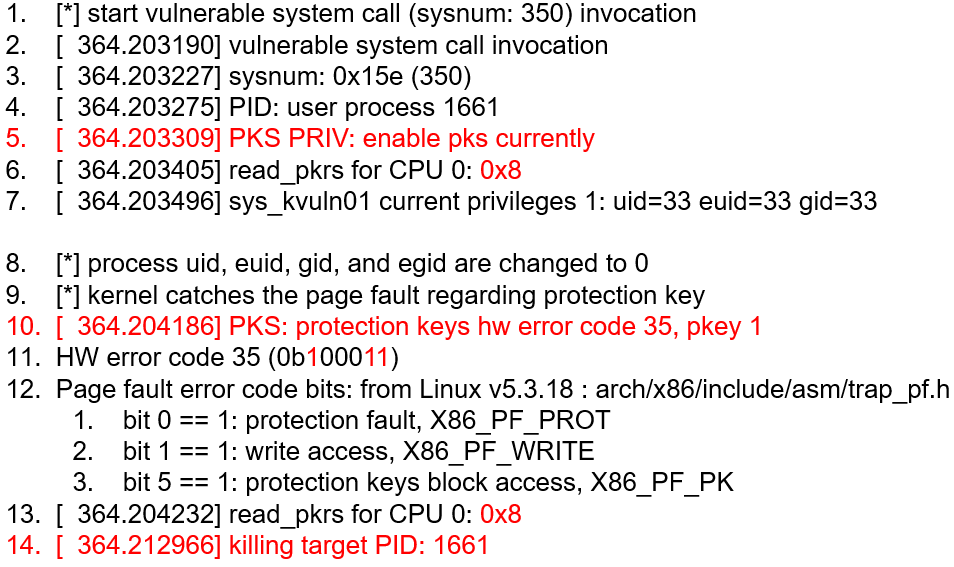
\includegraphics[bb=0 0 950 589, scale=.260]{./imgs/008_screenshot_2021-08-18_3.35.12.png}
%   \end{center}
%   \vspace{-2.0ex}
%   \caption{
%     %
%     特権奪取攻撃に利用可能なシステムコール捕捉時の動作結果
%     %
%   }
%   \vspace{-4.5ex}
%  \label{fig:kvuln1_1_04}
% \end{figure}


% \subsection{カーネル処理におけるオーバヘッド}
\subsection{Performance Evaluation Result}

\subsubsection{Measurement of the Kernel Processing Overhead:}

% 実現方式1のカーネル負荷として,システムコールのオーバヘッドの測定をベンチマーク
% ソフトウェア LMbench により評価した.LMbenchを実現方式1の適用前のLinux kernel と
% 適用したLinux kernelにてそれぞれ10回実行し,平均値からシステムコールのオーバヘッ
% ドを算出した.
The system call overhead was measured using LMbench benchmark software. 
%
A vanilla kernel was compared with the kernel with Implementation 1.
LMbench was executed 10 times to calculate the average system call latency.
% as the kernel load of the implementation method 1. 10 times LMbench was run on the
% Linux kernel before and after the application of the implementation method 1,
% respectively, and the average value was calculated as the system call overhead.

% 評価結果を表\ref{tb:evaluation_qemu_lmbench1}に示す.LMbench では, fork+/bin/sh
% は54回,fork+execveは4回,fork+exitは2回,open/close は2回,および,その他は1回
% のシステムコール呼出しを行う.
LMbench performs 54 invocations of the system call for fork+/bin/sh, 4 invocations
for fork+execve, 2 invocations for fork+exit and open/close, and the other is 1
invocation.
% %
% 表\ref{tb:evaluation_qemu_lmbench1}から,提案するセキュリティ機構の適用時におい
% て,最もオーバヘッドの発生したシステムコール処理はfork+execveであり,9.01\% %X.XXX $\mu$s
% を示した,また,最も少ないオーバヘッドはstatであり,2.96\%を示した.
% %
Table \ref{tb:evaluation_qemu_lmbench1} shows the overhead of the system call. The
highest and lowest overheads are fork+execve with 9.01\% and stat with 2.96\%,
respectively.

% -*- coding: utf-8; mode: latex; -*-
\begin{table}[t]
    \centering
    %  \caption{Overhead of MKM mechanism on the Linux kernel ($\mu$s)}
    \caption{System call invocation overhead of Implementation 1 ($\mu$s)}
  %  \vspace{-2.5ex}
    \scalebox{0.85}{
  
      \begin{tabular}{lrrr}
        \hline \noalign{\smallskip}
        \begin{tabular}{l}
          {\bf System call}
        \end{tabular}
        &
        \begin{tabular}{l}
          {\bf Vanilla kernel}
        \end{tabular}
        &
        \begin{tabular}{l}
          {\bf Implementation 1}
        \end{tabular}
        &
        \begin{tabular}{l}
          {\bf Overhead}
        \end{tabular}
        \\
        \noalign{\smallskip}
        \hline
        \noalign{\smallskip}
  fork+/bin/sh & 227111.28  & 236738.69  & 9627.41 (4.24\%)  \\
  fork+execve  & 12780.0566 & 13931.6703 & 1151.6136 (9.01\%)    \\
  fork+exit    & 10837.0729 & 11285.5603 & 448.4874 (4.14\%)    \\
  open/close   & 1302.5639  & 1334.5312  & 41.9672 (2.95\%)     \\
  read         & 168.8898   & 180.4594   & 11.5696 (6.85\%) \\
  write        & 164.2567   & 176.4273   & 12.1705 (7.41\%)     \\
  fstat        & 195.0063   & 203.7508   & 8.7445  (4.48\%)     \\
  stat         & 613.7426   & 631.9393   & 18.1966 (2.96\%)     \\
        
  \noalign{\smallskip}
  \hline
  \noalign{\smallskip}
      \end{tabular}
    }    
      \label{tb:evaluation_qemu_lmbench1}
  %  \vspace{-2.0ex}
  \end{table}
   % lmbench

% \subsection{PKS操作におけるオーバヘッド}
\subsubsection{Measurement of PKS Operations:}

% PKSの利用にかかる性能評価として,PKS操作に関するオーバヘッドを測定した.専用の測
% 定プログラムにおいて,カーネルにおけるPTEへのPkeyの設定ならびに PKRS 読書きを
% 10,000回繰返す処理を10回行い,平均値を測定した.
% %
% To evaluate the performance of using PKS, we measured the overhead associated
% with PKS operations.
% Measurement of the PKS operations. 
The Linux kernel with Implementation 2 invokes the Pkey write of the PTE and
read and write of the PKRS. The measurement program was repeated 10,000 times, and
the average value was calculated.
% 評価結果について表\ref{tb:evaluation_qemu_cpubench2}に示す.
% %
% Pkey の書込みには 30.5 ns ならびに PKRS の読込みに22.1 ns,書込みに
% 1347.9 nsのオーバヘッドを必要とすることを示した.
Table \ref{tb:evaluation_qemu_cpubench2} shows the cost of the PKS operations.
The write of Pkey required 30.5 ns; PKRS read required 22.1 ns, and PKRS
write required 1347.9 ns.
% was required.

%\begin{table}[t]
\hspace{-22.0ex}
\begin{tabular}{rl}    
  %\centering
   \begin{minipage}{0.8\hsize}    
    %  \caption{Overhead of MKM mechanism on the Linux kernel ($\mu$s)}
    \centering
    \caption{System call invocation overhead of Implementation 1 ($\mu$s)}
  %  \vspace{-2.5ex}
    \scalebox{1.0}{
  
      \begin{tabular}{lrrr}
        \hline \noalign{\smallskip}
        \begin{tabular}{l}
          {\bf System call}
        \end{tabular}
        &
        \begin{tabular}{l}
          {\bf Vanilla kernel}
        \end{tabular}
        &
        \begin{tabular}{l}
          {\bf Implementation 1}
        \end{tabular}
        &
        \begin{tabular}{l}
          {\bf Overhead}
        \end{tabular}
        \\
        \noalign{\smallskip}
        \hline
        \noalign{\smallskip}
  fork+/bin/sh & 227111.28  & 236738.69  & 9627.41 (4.24\%)  \\
  fork+execve  & 12780.0566 & 13931.6703 & 1151.6136 (9.01\%)    \\
  fork+exit    & 10837.0729 & 11285.5603 & 448.4874 (4.14\%)    \\
  open/close   & 1302.5639  & 1334.5312  & 41.9672 (2.95\%)     \\
  read         & 168.8898   & 180.4594   & 11.5696 (6.85\%) \\
  write        & 164.2567   & 176.4273   & 12.1705 (7.41\%)     \\
  fstat        & 195.0063   & 203.7508   & 8.7445  (4.48\%)     \\
  stat         & 613.7426   & 631.9393   & 18.1966 (2.96\%)     \\
        
  \noalign{\smallskip}
  \hline
  \noalign{\smallskip}
      \end{tabular}
    }    
      \label{tb:evaluation_qemu_lmbench1}

   \end{minipage}
   \hspace{8mm}
   \begin{minipage}{0.7\hsize}
    \centering
    \caption{PKS operations overhead of Implementation 2 (ns)}
  %  \vspace{-2.5ex}
    \scalebox{1.0}{
  
      \begin{tabular}{lr}
        % \hline
        \hline \noalign{\smallskip}
        % \hline
        \begin{tabular}{l}
          {\bf Instruction}
        \end{tabular}
        &
        \begin{tabular}{l}
          % {\bf Our proposed mechanism}
          {\bf Implementation 2}
         \end{tabular}
          \\
          \noalign{\smallskip}          
          \hline
          \noalign{\smallskip}
          %Total        & 349.260 \\
          % Pkey read    & 0.xxx  \\
          % Pkey write   & 30.5263  \\
          % PKRS read    & 22.1052  \\
          % PKRS write   & 1347.8965  \\
          Pkey write   & 30.5  \\
          PKRS read    & 22.1  \\
          PKRS write   & 1347.9  \\
          
        \noalign{\smallskip}          
        \hline
        \noalign{\smallskip}          
      \end{tabular}
    }    
      \label{tb:evaluation_qemu_cpubench2}
  \end{minipage}
\end{tabular}
\end{table}
% -*- coding: utf-8; mode: latex; -*-
\begin{table}[t]
    \centering
    %  \caption{Overhead of MKM mechanism on the Linux kernel ($\mu$s)}
    \caption{Overhead of PKS operations (ns)}
  %  \vspace{-2.5ex}
    \scalebox{1.0}{
  
      \begin{tabular}{lr}
        % \hline
        \hline \noalign{\smallskip}
        % \hline
        \begin{tabular}{l}
          {\bf Instruction}
        \end{tabular}
        &
        \begin{tabular}{l}
          % {\bf Our proposed mechanism}
          {\bf Implementation 2}
         \end{tabular}
          \\
          \noalign{\smallskip}          
          \hline
          \noalign{\smallskip}
          %Total        & 349.260 \\
          % Pkey read    & 0.xxx  \\
          % Pkey write   & 30.5263  \\
          % PKRS read    & 22.1052  \\
          % PKRS write   & 1347.8965  \\
          Pkey write   & 30.5  \\
          PKRS read    & 22.1  \\
          PKRS write   & 1347.9  \\
          
        \noalign{\smallskip}          
        \hline
        \noalign{\smallskip}          
      \end{tabular}
    }    
      \label{tb:evaluation_qemu_cpubench2}
  %  \vspace{-2.0ex}
  \end{table} % cpu cycle

\subsubsection{Measurement of the Kernel Instruction Increasing:}
The Linux kernel with implementations require protected kernel data management
and handling of write restrictions that contain the instructions of PKS
operations.
%
% The original LKM only contains Pkey write, read, PKRS read and write for the
% measurement of the instructions of PKS operations.
% that contains Pkey and PKRS read, write.
%
For the calculation of the instruction increasing, both implementations extract
the additional kernel code to the source code file, then vanilla kernel only
contains the invocation placement (e.g., function call) of both implementations.
% using same Linux kernel config file.
The disassemble tool calculates instructions for the object files of each
implementation.

% %
Table \ref{tb:evaluation_instructions} shows the increasing instruction.
Implementation 1 requires 176 instructions and Implementation 2 requires 137
instructions.
%  Additionally, PKS operations requires xxx instructions
%
% Additionally, 
%  for both implementations.
% the PKS operations.
% The write of Pkey required 30.5 ns; PKRS read required 22.1 ns, and PKRS
% write required 1347.9 ns.
% -*- coding: utf-8; mode: latex; -*-
\begin{table}[t]
    \centering
    %  \caption{Overhead of MKM mechanism on the Linux kernel ($\mu$s)}
    \caption{Increasing of instructions on the Linux kernel}
  %  \vspace{-2.5ex}
    \scalebox{1.0}{
  
      \begin{tabular}{lrr}
        % \hline
        \hline \noalign{\smallskip}
        % \hline
        % \begin{tabular}{l}
        %   {\bf Instruction}
        % \end{tabular}
        &
        \begin{tabular}{l}
          % {\bf Our proposed mechanism}
          {\bf Implementation 1}
         \end{tabular}
         &
         \begin{tabular}{l}
            % {\bf Our proposed mechanism}
            {\bf Implementation 2}
           \end{tabular}         
        %    &
        %    \begin{tabular}{l}
        %     % {\bf Our proposed mechanism}
        %     {\bf PKS operation}
        %    \end{tabular}                    
          \\
          \noalign{\smallskip}          
          \hline
          \noalign{\smallskip}
          %Total        & 349.260 \\
          % Pkey read    & 0.xxx  \\
          % Pkey write   & 30.5263  \\
          % PKRS read    & 22.1052  \\
          % PKRS write   & 1347.8965  \\
          % Instructions   & xxx.xxx & xxx.xxx \\
          Instructions   & 176 & 137 \\
        %   PKRS read    & 22.1  \\
        %   PKRS write   & 1347.9  \\
          
        \noalign{\smallskip}          
        \hline
        \noalign{\smallskip}          
      \end{tabular}
    }    
      \label{tb:evaluation_instructions}
  %  \vspace{-2.0ex}
  \end{table} % lmbench


% \subsubsection{Implementation}
% %
% %\reduline{
% vkTracer was implemented on the Linux x86\_64 CPU kernel.
% %
% To evaluate the tracing capability, two known kernel vulnerabilities
% were introduced into Linux kernel 5.0.0 using an actual kernel
% vulnerability and PoC code \cite{CVE-2017-6074, CVE-2017-16995}.
% %
% One kernel vulnerability leads to privilege escalation via memory corruption,
% and the other leads to DoS on the running kernel:

% \begin{itemize}
  
%   %\item {\bf Memory Corruption}: The vulnerable kernel code 1 is
% \item {\bf Privilege escalation}: Vulnerable kernel code 1 refers to
%   CVE-2017-6074 \cite{CVE-2017-6074}, which was implemented as system
%   call \verb|sys_kvuln01|, \verb|support_sys_kvuln01_01|, and
%   \verb|support_sys_kvuln01_02|.
%   %
%   PoC code 01 exploits these functions to overwrite the credential
%   information of a user process to achieve privilege escalation.
%   %% カーネル脆弱性1(バッファオーバーフロー):独自システムコール1の
%   %% 実行中,カーネル脆弱性1を含むカーネルコード1-1,1-2を呼出す.ユーザ
%   %% プロセスの権限情報をバッファオーバーフローにより改竄し,特権奪取可能
%   %% とする.

% \item {\bf DoS}:
%   %\item カーネル脆弱性2(解放済みメモリの参照):
%   Vulnerable kernel code 2 refers to CVE-2017-16995 \cite{CVE-2017-16995}, which was
%   implemented as system call \verb|sys_kvuln02| and
%   \verb|support_sys_kvuln02_01|.
%   %
%   PoC code 02 exploits these functions to forcibly free a variable and then free it
%   again (e.g., double free of UAF). The \verb|sys_kvuln02| forces a DoS
%   on the running kernel.
  
%   %% 独自システムコール2の実
%   %% 行中にメモリ領域を確保,カーネルコード2-1を呼出し,該当メモリ領域を
%   %% 開放する.その後,独自システムコール2にて,開放済みメモリ領域を参照
%   %% し,DoS を発生させる.


% \end{itemize}

% %
% In addition, to evaluate the performance cost, vkTracer calculated the
% execution times of the PoC codes. vkTracer required 712 lines for the
% application. The proven kernel vulnerabilities required 192 lines for four
% files, whereas the PoC code for the Linux kernel 5.0.0 had 143 lines.

% \subsection{Identification of Vulnerable Kernel Code} 
% \subsubsection{Case of Privilege Escalation}
% %The left side of Figure \ref{fig:kvuln1_1}
% Figure \ref{fig:kvuln1_1}
% %
% shows that the adversary's user process attempted to invoke the
% %
% \verb|support_kvuln01_01| and \verb|support_kvuln01_02| functions
% during the \verb|sys_kvuln1| system call in lines 6 to 8.
% %
% vkTracer was able to trace and identify the invocation of
% vulnerable kernel codes.% at this time.
% %
% The adversary's user process upgraded from a normal user account (e.g., user id
% is 1000) to obtain the administrator account privilege, as shown by the user
% process id (e.g., user id is 0) at line 10. 
% % changing from the normal user account (e.g., user id is 1000) at line 10.
% %
% Then, vkTracer determined the function names and virtual address ranges
% of the vulnerable kernel codes in lines 18 to 20. This tracing
% result was correct, shown by the symbol information in line 28 to 30.
% %
% Finally, vkTracer generated the profile of \verb|sys_kvlun1| and other functions
% in line 31 to 33.



% \subsubsection{Case of DoS}
% %The right side of Figure \ref{fig:kvuln1_2}
% Figure \ref{fig:kvuln1_2}
% %
% shows that the adversary's user process attempted to invoke the
% %
% \verb|support_kvuln02| and \verb|support_kvuln02_01| functions in lines
% 4 to 7,
% %
% after which the running kernel was terminated. Subsequently, in lines 9 to 10,
% vkTracer determined the function names and virtual address ranges of the
% vulnerable kernel codes at the remote server. This tracing
% result was correct, shown by the symbol information in lines 14 to 15.
% %
% Finally, vkTracer generated the profile of \verb|sys_kvlun2| and
% \verb|support_kvuln02_01| in lines 16 and 17.

% Therefore, vkTracer identified the vulnerable kernel codes and
% extracted the kernel code information as a profile containing the
% function name and virtual address range.


% \subsection{Measurement of The Performance Cost}

% \subsubsection{Measurement of Vulnerable Kernel Code Identification}
% To evaluate the tracing overhead, the processing costs of a vanilla kernel
% and vkTracer were compared.
% %
% The tracing overhead is a measure of the processing time of PoC codes
% that exploit proven kernel vulnerabilities.
% %
% The kernel compilations were run five times to determine the average
% processing time of two different PoC codes as the user process.
% %
% Table \ref{tb:evaluation_physical_kernel} lists the performance scores.
% vkTracer required 5.2728 s and 5.2683 s for the two PoC codes.%, respectively.


% \subsubsection{Measurement of The Kernel Overhead}
% To measure the kernel performance overhead, LMbench was executed five
% times to determine the average system call overhead between a vanilla
% kernel and a kernel with vkTracer.

% LMbench invokes two system call counts for open/close and the other
% system calls count is one.
% %
% Table \ref{tb:evaluation_physical_lmbench} shows that the open/close
% system calls are the highest overhead for vkTracer, i.e., 7.4394 $\mu$s
% (3.7197 $\mu$s for each once), whereas the fstat system call has the
% lowest overhead, i.e., 3.2292 $\mu$s.


% \subsubsection{Measurement of Application Overhead}
% To measure the tracing overhead for the web application,
% %
% the web server nginx 1.21.4 was used, and the benchmark web client was
% ApacheBench 2.4.
% %The web server used was nginx 1.21.4.  The benchmark web client was
% %ApacheBench 2.4.
% The network environment was 1 Gbps.
% %
% % The benchmark configuration adopted the relevant the ApacheBench sending 100,000
% The adopted benchmark configuration involved ApacheBench sending 100,000 HTTP
% accesses and then downloading files for one connection, with file sizes of 1 kB,
% 10 kB, and 100 kB.
% %

% Table \ref{tb:evaluation_physical_apachebench} shows the
% calculation result of the HTTP download request average.
% %
% vkTracer has an average overhead between 0.37 \% and 0.56 \% for each file
% download access.

% %The web application process used was an  web server.
% %The benchmark adopted 
% %for HTTP accesses. 
% %and KPRM implementation 2 has an average overhead of 1.188 \% to 3.008 \% 

%     %\vspace{-4.0ex}
%     %\end{table}
% \begin{table}[t]
%   \centering
%       %\begin{table}[tb]
% %  \vspace{-1.0ex}
%   \caption{Tracing overhead of vkTracer (s)}
% %  \vspace{-1.2ex}          
%         %  \vspace{-2.0ex}
%   \label{tb:evaluation_physical_kernel}
%   \scalebox{0.98}{
%     %  \begin{tabular}{r|r|r|r}
%     \begin{tabular}{lrrr}
%       \hline
% \noalign{\smallskip}      
%       %\begin{tabular}{l}
%       %\end{tabular}
%       %&
%       \begin{tabular}{l}
%         {\bf Application}
%       \end{tabular}
%       &
%       \begin{tabular}{l}
%         {\bf Vanilla kernel}
%       \end{tabular}
%       &
%       \begin{tabular}{l}
%         {\bf w/ vkTracer}
%       \end{tabular}
%       &
%       \begin{tabular}{l}
%         {\bf Overhead}
%       \end{tabular}
%       \\
% \noalign{\smallskip}      
% \hline
% \noalign{\smallskip}
%       PoC code 01  & 0.2047 & 5.4775 & 5.2728 \\            
%       PoC code 02  & 0.1034 & 5.3717 & 5.2683 \\
%       \hline
%     \end{tabular}
%   }
%   %\vspace{-4.0ex}
%   %\end{table}
%   %\vspace{-4.0ex}
% \end{table}

% \begin{table}[t]
%   \centering
%   %\vspace{-1.0ex}
%   \caption{One time system call invocation overhead of vkTracer ($\mu$s)}
%   %\vspace{-1.1ex}  
% %  \vspace{-2.5ex}
%   \scalebox{0.95}{

%     %\begin{tabular}{l|r|r|r}
%     \begin{tabular}{lrrr}
% %      \hline
%       \hline
% \noalign{\smallskip}      
%       \begin{tabular}{l}
%         {\bf System call}
%       \end{tabular}
%       %% &
%       &
%       \begin{tabular}{l}
%         {\bf Vanilla kernel}
%       \end{tabular}
%       &
%       \begin{tabular}{l}
%         {\bf w/ vkTracer}
%       \end{tabular}
%       &
%       \begin{tabular}{r}
%         {\bf Overhead}
%       \end{tabular}        
%         \\
% \noalign{\smallskip}
% \hline
% \noalign{\smallskip}

% open/close & 1.6049 & 9.0443  & 7.4394\\ 
% read	     & 0.3545 & 4.0560  & 3.7015\\
% write	     & 0.2997 & 3.5443  & 3.2446\\
% stat	     & 0.5831 & 3.9714  & 3.3883\\
% fstat	     & 0.4068 & 3.6360  & 3.2292\\

      
%       \hline
%     \end{tabular}
%     \label{tb:evaluation_physical_lmbench}
%   }
%   %\vspace{-2.5ex}
% \end{table}

% \begin{table}[t]
%   \centering  
% %  \begin{center}
% %    \hspace*{-15.0ex}
%   %\begin{tabular}{cc}    
%       %\begin{table}[tb]
% %      \begin{center}  
% %    \vspace{-1.0ex}
%     \caption{ApacheBench overhead of vkTracer ($\mu$s).}
% %    \vspace{-1.2ex}            
%     \label{tb:evaluation_physical_apachebench}
%     \scalebox{1.00}{
%       %\begin{tabular}{ r|r|r|r}
%       \begin{tabular}{rrr}
%         \hline
% \noalign{\smallskip}        
%         \begin{tabular}{l}
%           {\bf File size (kB)}
%         \end{tabular}
%         &
%         \begin{tabular}{l}
%           {\bf Vanilla kernel}
%         \end{tabular}
%         &
%         \begin{tabular}{l}
%           {\bf w/ vkTracer}
%         \end{tabular}
%         \\
% \noalign{\smallskip}
% \hline
% \noalign{\smallskip}

%         1    & 648.769   & 651.182   (0.37 \%)\\ %  106.172
%         10   & 1,091.750 & 1,097.833 (0.56 \%)\\
%         100  & 2,620.545 & 2,630.538 (0.38 \%)\\

%         %10   & 1,227.692 & 1,003.583 (18.25\%)\\
%         %10   & 1,086.111 & 1,091.000 & 99.55\%\\ & 0.004889
%         %10   & 1.086667  & 1.097833 (1.03 \%)\\ & 0.011166
%         \hline
%       \end{tabular}
%     }
%     %\vspace{-4.0ex}
% \end{table}


%% To evaluate tracing and identification cost, the processing cost of
%% the vanilla and vkTracer were compared.
%% %
%% The tracing and identification overheads measures the processing time
%% of PoC codes that exploits proven kernel vulnerabilities.
%% %
%% The kernel compilations were run five times to determine the average
%% user process processing time.
%
%Table \ref{tb:evaluation_physical_kernel} indicates that
%vkTracer had overheads of Z.XX \% and Z.YY \%, respectively.
%
%in a general application execution environment.d
%
%The compile target was Linux kernel 5.0.0 source code with Debian 10.0
%kernel configuration (e.g., default .config file).



%% To evaluate the processing time for system environment, sysbench
%% compares the vanilla kernel and the kernel with vkTracer.
%% %
%% The benchmark setting was 4 threads and 20,000 prime calculation,
%% 100GB memory sequential access, and 2GB file random read / write.
%% %
%% %
%% %Table \ref{tb:evaluation_physical_kernel} indicates that
%% The performance scores are presented in
%% Table \ref{tb:evaluation_sysbench}. vkTracer had processing performance
%% of 72.74 \% to 94.84 \%, respectively.

%% \begin{table}[tb]
%%   \centering
%%       %\begin{table}[tb]
%% %  \vspace{-1.0ex}
%%   \caption{System overhead of vkTracer (operations/s)}
%% %  \vspace{-1.2ex}          
%%         %  \vspace{-2.0ex}
%%   \label{tb:evaluation_sysbench}
%%   \scalebox{1.0}{
%%     %  \begin{tabular}{r|r|r|r}
%%     \begin{tabular}{r|r|r}
%%       \hline
%%       %\begin{tabular}{l}
%%       %\end{tabular}
%%       %&
%%       \begin{tabular}{l}
%%         Target
%%       \end{tabular}
%%       &
%%       \begin{tabular}{l}
%%         Vanilla kernel
%%       \end{tabular}
%%       &
%%       \begin{tabular}{l}
%%         Kernel w/ vkTracer
%%       \end{tabular}
%%       \\
%%       \hline
%%       CPU         & 1526.01    & 1194.14    (21.75 \%) \\ %(78.25 \%)
%%       Memory      & 3077067.32 & 2918245.29 (5.16 \%) \\ % 4 thread, 4k block, 100GB transfer, seq access (94.84 \%)
%%       Disk read   & 11418.39   & 8306.24    (27.26 \%) \\ %(72.74 \%)
%%       Disk write  & 7612.23    & 5537.49    (27.26 \%)  \\ %(72.74 \%)
%%       \hline
%%     \end{tabular}
%%   }
%%   %\vspace{-4.0ex}
%%   %\end{table}
%%   %\vspace{-4.0ex}
%% \end{table}



%\subsubsection{Identification of vulnerable kernel code}

%% \item カーネル脆弱性1(バッファオーバーフロー):独自システムコール1の
%%   実行中,カーネル脆弱性1を含むカーネルコード1-1,1-2を呼出す.ユーザ
%%   プロセスの権限情報をバッファオーバーフローにより改竄し,特権奪取可能
%%   とする.


%% 図\ref{fig:kvuln1_1}にカーネル脆弱性1を介して攻撃を行うユーザプロセス
%% の追跡結果を示す.

%% %図\ref{fig:kvuln1_1},
%% 攻撃実行前のユーザプロセスは通常ユーザの権限(ユーザID 1,000)であるこ
%% とが2行目にて表示されている.
%% %
%% %% 攻撃成功時側は,図\ref{fig:kvuln1_1}x
%% 6行目から8行目にて,独自システムコール1を呼出し,カーネル脆弱性1を利用
%% するカーネルコード1-1,および1-2の呼出しについて,追跡結果が表示されて
%% いる.
%% %
%% 独自システムコール1の終了後,10行目にてユーザプロセスは特権奪取(ユー
%%   ザID 0)に成功しており,同時に提案手法の追跡は終了したことを確認でき
%% る.

%% カーネルコードの仮想アドレス範囲の特定結果として,13行目から26行目にか
%% け,提案手法にてユーザプロセスの追跡により収集したカーネルコードと仮想
%% アドレスの組合せを表示している.18行目から20行目にかけては攻撃実行時の
%% みに収集されたカーネルコードであり,独自システムコール1およびカーネル
%% 脆弱性1を含むカーネルコード1-1,1-2の仮想アドレス範囲を特定している.
%% %できていることを確認できる.
%% %
%% %また,図\ref{fig:kvuln1_1}25行目からxx行目にかけ,攻撃成功時のみのカー
%% また,28行目から30行目は,カーネルイメージに含まれるシンボル情報から攻
%% 撃実行時のみに呼出されるカーネルコードと仮想アドレスの組合せを抽出した
%% 結果である.提案手法において特定した開始仮想アドレスと同値であるこ
%% とを確認できる.


%% \subsubsection{Prevention of vulnerable kernel code access and kernel memory corruption}  \label{subseciton:evaluation_restricted}
%% \blueuline{ The evaluation of practical security capability is to
%%   prevent the invocation of vulnerable kernel code and protect
%%   privilege kernel data on the implementation 1 of KPRM kernel through the eBPF kernel
%%   attack with CVE-2017-16995} in \cite{CVE-2017-16995}.
%% %
%% \blueuline{The modified PoC code can overwrite any kernel virtual
%%   address.}  The PoC code invokes \verb|sys_bpf| system call that
%% calls the \verb|map_update_elem| kernel code to execute the
%% malicious code; then after It tries to modify the \verb|cred| variable
%% of the privilege kernel data of the running user process.
%% %
%% \blueuline{
%%   The implementation 1 of KPRM kernel adopts the profile of the modified PoC code that
%%   prepares the restricted kernel page containing the vulnerable kernel code}
%% \verb|map_update_elem| and targeted privilege kernel data of \verb|cred| variable.

%% %% The prevention of vulnerable kernel code invocation and the protection
%% %% of privilege kernel data on the KPRM kernel is achieved through the
%% %% eBPF kernel attack with CVE-2017-16995 \cite{CVE-2017-16995}.
%% %% %
%% %% The PoC code invokes \verb|the map_update_elem| function to execute
%% %% the malicious code to try to modify the \verb|cred| variable of the
%% %% privilege kernel data of the running user process at the
%% %% \verb|sys_bpf| system call.
%% %% %
%% %% The KPRM kernel prepares the restricted kernel page containing the
%% %% vulnerable kernel code and targeted privilege kernel data.

%% Figure \ref{fig:exclusive_kernel_code_evaluation} shows that the
%% adversary's user process tries to invoke the \verb|map_update_elem|
%% function during the \verb|sys_bpf| system call processing at line
%% 5. The restriction of KPRM proceeds with the restricted kernel
%% page handling at line 6; thereafter, it can catch the page fault that
%% contains the virtual address of the vulnerable kernel code. In this
%% situation, the KPRM kernel determines the running process that
%% requests invalid access to the restricted kernel page and then sends
%% SIGKILL to stop the adversary's user process.

%% Figure \ref{fig:exclusive_kernel_data_evaluation_attack_failure} shows
%% the prevention success case of memory corruption. The user
%% \verb|www-data| with user id 33 also executes the PoC code at line
%% 1. The adversary's user process tries to modify the \verb|cred| struct
%% of the privilege kernel data to the root with user id 0 at lines 9 to
%% 11. The restriction of KPRM kernel automatically restricts the
%% access of the adversary's user process to the privilege kernel data on
%% the restricted kernel page. Finally, the adversary's user process runs
%% the shell program without administrator privilege at line 14.

%% \blueuline{
%% From the results, implementation 1 of KPRM kernel can prohibit
%% vulnerable kernel code invocation and protect the privilege kernel
%% data to prevent memory corruption from the eBPF kernel attack with
%% CVE-2017-16995 with the stable behavior for running the kernel and
%% user process. Implementation 2 of KPRM kernel also can only prohibit
%% vulnerable kernel code invocation at the same evaluation environment.
%% }

%% \begin{figure}[t]
%% %  \begin{center}
%% %  \hspace*{-8.0ex}    
%% %    \begin{tabular}{cc}
%% %      \begin{minipage}[t]{0.65\hsize}
%%         \begin{center}
%%           \includegraphics[bb=0 0 971 596, scale=.255]{./imgs/010_screen_shot_2019-08-16_3.45.02.png}
%%         \end{center}
%% %        \vspace{-1.0ex}
%%         \caption{
%%           %Prevention of kernel code calling with restricted kernel page
%%           Attack prevention case of vulnerable kernel code invocation
%%         }
%% %        \vspace{-1.5ex}
%%         \label{fig:exclusive_kernel_code_evaluation}
%% %      \end{minipage} & %\hspace{10.0ex}
%% \end{figure}

%% \begin{figure}[t]    
%% %      \begin{minipage}[t]{0.65\hsize}
%%         \begin{center}
%%           \includegraphics[bb=0 0 991 705, scale=.255]{./imgs/009_screen_shot_2020-06-16_16.43.47.png}
%%         \end{center}
%% %        \vspace{-1.0ex}
%%         \caption{
%%           Attack prevention case of kernel data access
%%         }
%% %        \vspace{-1.5ex}
%%         \label{fig:exclusive_kernel_data_evaluation_attack_failure}
%% %      \end{minipage}
%% %    \end{tabular}
%% %  \end{center}
%%   %\vspace{-4.0ex}  
%% \end{figure}



%% \subsection{Measurement of Performance Overhead}

%% \subsubsection{Measurement of System Call Overhead}
%% %
%% \blueuline{
%% For the measurement of the performance overhead, the comparison of
%% between a vanilla kernel and KPRM kernel. The benchmark software
%% LMbench was executed 10 times to determine the average system call
%% overhead.
%% %
%% The result was the overhead time of kernel with KPRM that
%% incurs a kernel page handling cost for each system call invocation.}

%% \reduline{
%% The LMbench invokes the different system calls counts (i.e., open /close is two times and
%% remaining system call is one time invocation).}
%% %
%% Table \ref{tb:evaluation_physical_lmbench}
%% \blueuline{
%% shows that the stat system
%% call has the highest overhead for implementation 1 and 2 of KPRM
%% (0.703 $\mu$s and 0.626 $\mu$s), whereas the write system call has the
%% lowest overhead (0.617 $\mu$s and 0.557 $\mu$s).}
%% %summarizes the lmbench result for each system call invocation.

%% \begin{table*}[t]
%%   \centering
%%   %\vspace{-1.0ex}
%%   \caption{One time system call invocation overhead of KPRM kernel ($\mu$s)}
%%   %\vspace{-1.1ex}  
%% %  \vspace{-2.5ex}
%%   \scalebox{1.0}{

%%     %\begin{tabular}{l|r|r|r}
%%     \begin{tabular}{lrrr}
%% %      \hline
%%       \hline
%%       \begin{tabular}{l}
%%         System call
%%       \end{tabular}
%%       %% &
%%       &
%%       \begin{tabular}{l}
%%         Vanilla kernel
%%       \end{tabular}
%%       &
%%       \begin{tabular}{l}
%%         Implementation 1 
%%       \end{tabular}
%%       &
%%       \begin{tabular}{r}
%%         Implementation 2
%%       \end{tabular}        
%%         \\
%%       \hline

%% open/close & 0.532 & 1.187 (0.655) & 1.119 (0.587)\\ % 0.6545, 0.5865
%% read	   & 0.276 & 0.896 (0.620) & 0.838 (0.562)\\
%% write	   & 0.238 & 0.856 (0.617) & 0.796 (0.557)\\
%% stat	   & 0.547 & 1.251 (0.703) & 1.173 (0.626)\\
%% fstat	   & 0.291 & 0.938 (0.647) & 0.873 (0.582)\\

      
%%       \hline
%%     \end{tabular}
%%     \label{tb:evaluation_physical_lmbench}
%%   }
%%   %\vspace{-2.5ex}
%% \end{table*}


%% \subsubsection{Measurement of Application Overhead}
%% \blueuline{
%% The measurement of the web application process overhead 
%% for the vanilla kernel and KPRM kernel.
%% %
%% The web application process used was an Apache 2.4.25 web server. The
%% benchmark software was ApacheBench 2.4 for the web client. The network
%% environment was 1 Gbps.
%% %
%% ApacheBench 2.4 calculated the HTTP download request
%% average for HTTP accesses. The benchmark configuration of ApacheBench
%% sent 100,000 HTTP accesses, then downloaded file for one connection.
%% The benchmark adopted files sizes is 1 KB, 10 KB, and 100 KB.
%% %
%% As listed in Table} \ref{tb:evaluation_physical_apachebench} indicates that
%% implementation 1 of the KPRM kernel has an average overhead of 2.617
%% \% - 4.093 \% and the implementation 2 of the KPRM kernel has an
%% average overhead of 1.188 \% - 3.008 \% for each file download access.

%% \subsubsection{Measured of Kernel Processing Overhead}
%% \blueuline{
%% To evaluate kernel processing overhead, kernel compilation times
%% involved comparison between the vanilla kernel and the KPRM kernel.
%% %
%% The kernel compiling overhead measures the processing time of specific
%% applications (i.e., compiler and linker) in a general application
%% execution environment.
%% %
%% The compile target was Linux kernel 5.0.0 source code with Debian 9.0
%% kernel configuration (e.g., default .config file). The kernel
%% compilations were five times to determine the average kernel
%% processing time.
%% %
%% %Table \ref{tb:evaluation_physical_kernel} indicates that
%% Implementation 1 and 2 of the KPRM kernel had kernel compiling
%% overhead of 2.459 \% and 2.193 \%, respectively, the performance score
%% as presented in Table} \ref{tb:evaluation_physical_kernel}.
        
%% \begin{table*}[tb]
%%   \centering  
%% %  \begin{center}
%% %    \hspace*{-15.0ex}
%%   %\begin{tabular}{cc}    
%%       %\begin{table}[tb]
%% %      \begin{center}  
%% %    \vspace{-1.0ex}
%%     \caption{ApacheBench overhead of KPRM kernel ($\mu$s).}
%% %    \vspace{-1.2ex}            
%%     \label{tb:evaluation_physical_apachebench}
%%     \scalebox{1.0}{
%%       %\begin{tabular}{r|r|r|r}
%%       \begin{tabular}{rrrr}
%%         \hline
        
%%         \begin{tabular}{l}
%%           File size (KB)
%%         \end{tabular}
%%         &
%%         \begin{tabular}{l}
%%           Vanilla kernel
%%         \end{tabular}
%%         &
%%         \begin{tabular}{l}
%%           Implementation 1
%%         \end{tabular}
%%         & Implementation 2\\
%%         \hline
        
%%         1  & 599.143   & 623.667   (4.093 \%)  & 617.167  (3.008 \%)\\
%%         10 & 764.250   & 784.250   (2.617 \%)  & 773.333  (1.188 \%)\\
%%         100& 2,443.714 & 2,509.167 (2.678 \%)  & 2502.667 (2.412 \%)\\
            
%%         \hline
%%       \end{tabular}
%%     }
%%     %\vspace{-4.0ex}
%% \end{table*}
    
%%     %\vspace{-4.0ex}
%%     %\end{table}
%% \begin{table}[tb]
%%   \centering
%%       %\begin{table}[tb]
%% %  \vspace{-1.0ex}
%%   \caption{Kernel building overhead of KPRM kernel (s)}
%% %  \vspace{-1.2ex}          
%%         %  \vspace{-2.0ex}
%%   \label{tb:evaluation_physical_kernel}
%%   \scalebox{1.0}{
%%     %  \begin{tabular}{r|r|r|r}
%%     \begin{tabular}{r|r|r}
%%       \hline
%%       %\begin{tabular}{l}
%%       %\end{tabular}
%%       %&
%%       \begin{tabular}{l}
%%         Vanilla kernel
%%       \end{tabular}
%%       &
%%       \begin{tabular}{l}
%%         Implementation 1
%%       \end{tabular}
%%       &
%%       \begin{tabular}{l}
%%         Implementation 2
%%       \end{tabular}
%%       \\
%%       \hline      
%%       5926.644 (s)  & 6072.413 (2.459 \%)  & 6056.629 (2.193 \%) \\
%%       \hline
%%     \end{tabular}
%%   }
%%   %\vspace{-4.0ex}
%%   %\end{table}
%%   %\vspace{-4.0ex}
%% \end{table}



%% %% \begin{table}[tb]
%% %%   \centering
%% %%       %\begin{table}[tb]
%% %% %  \vspace{-1.0ex}
%% %%   \caption{Unixbench score of KPRM kernel}
%% %% %  \vspace{-1.2ex}          
%% %%         %  \vspace{-2.0ex}
%% %%   \label{tb:evaluation_physical_unixbench}
%% %%   \scalebox{1.0}{
%% %%     %  \begin{tabular}{r|r|r|r}
%% %%     \begin{tabular}{r|r|r}
%% %%       \hline
%% %%       %\begin{tabular}{l}
%% %%       %\end{tabular}
%% %%       %&
%% %%       \begin{tabular}{l}
%% %%         Vanilla kernel
%% %%       \end{tabular}
%% %%       &
%% %%       \begin{tabular}{l}
%% %%         Implementation 1
%% %%       \end{tabular}
%% %%       &
%% %%       \begin{tabular}{l}
%% %%         Implementation 2
%% %%       \end{tabular}
%% %%       \\
%% %%       \hline
%% %%       1380.060        & 1347.617 (2.35\%) & 1347.617 (2.35\%) \\      
%% %%       %5926.644 (s)  & 6072.413 (2.459 \%)  & 6056.629 (2.193 \%) \\
%% %%       \hline
%% %%     \end{tabular}
%% %%   }
%% %%   %\vspace{-4.0ex}
%% %%   %\end{table}
%% %%   %\vspace{-4.0ex}
%% %% \end{table}

% The capability assessment of vkTracer was validated by
% identifying the vulnerable kernel code. 
% %the identification of 
% %% is validated by identification
% %% of vulnerable kernel code.  Additionally, the performance evaluation
% %% is to measure the overhead cost for kernel and user process.
%   %of the vkTracer
% %and prevention of kernel memory corruptions.
% %to evaluate the security capability of the MKM kernel.
% %}

% \begin{enumerate}%[leftmargin=0.5cm]%\itemsep=-1.0ex \parskip=1.0ex

%   \item {\bf Identification of vulnerable kernel code}:
%     %
%     The ability of vkTracer to identify vulnerable kernel code
%     information, when an adversary's user process attempts to exploit
%     a proven kernel vulnerability when invoking a system call, was
%     evaluated.
%   %
%  % \reduline{    
%     %% %The evaluation of
%     %% Evaluating whether vkTracer can identify
%     %% vulnerable kernel code information when an adversary's user process
%     %% attempts to exploit an proven kernel vulnerability when invoking a system call.
%     %  }
% \end{enumerate}
% , tracing, identification, kernel, and user process overhead costs were measured.
    %KPRM kernel using Linux kernel compilation time.
    %  }

%% \item {\bf Prevention of vulnerable kernel code access and kernel memory corruption:}
%%   %  
%%   The evaluation of whether the restriction of KPRM kernel can
%%   prevent vulnerable kernel code execution and protect kernel data of
%%   privilege information when an adversary's user process tries to
%%   exploit an actual kernel vulnerability at system call invocation.
%%   %

%% \subsection{Performance Measurement}
%% %\subsection{Purpose and Environment}

%% The performance evaluation objectives are to measure
%% overhead cost for the user process and a vanilla
%% kernel and the KPRM kernel.

%% %  \vspace{-1.0ex}
%% \begin{enumerate}[leftmargin=0.5cm]%\itemsep=-1.0ex \parskip=1.0ex

%% \item {\bf Measurement of the system call invocations overhead:}
%%   To measure the implementation effect for KPRM kernel feasibility, a
%%   benchmark software was used to calculate the overhead of system call
%%   invocation latency.

%% \item {\bf Measurement of application overhead:}
%%   The performance overhead for the application was measured using a
%%   web benchmark software and
%%   %
%%   %kernel compilation of Linux kernel on the KPRM kernel.

%% \item {\bf Measured of kernel processing overhead:}
%%   %
%%   \reduline{
%%   The processing performance overhead of the KPRM kernel using Linux
%%   kernel compilation time.
%%   }
%%   %
%% \end{enumerate}
%% %\vspace{-1.0ex}
%
%% To evaluate the tracing capability, two proven kernel
%% vulnerabilities are introduced into the Linux kernel 5.0.0.
%% %
%% One kernel vulnerability leads privilege escalation, and other leads
%% DoS on the running kernel.
%% %
%% Additionally, to evaluate the performance cost,
%% vkTracer calculates the execution times of PoC codes.
%% %}
%% %
%% %\reduline{
%% The vkTracer required 712 lines for the application.
%% %
%% The proven kernel vulnerabilities required 192 lines for 4 files
%% and PoC code was 143 lines to the Linux kernel 5.0.0.
%}
%Additionally, to evaluate the practical security capability of KPRM,
%actual kernel vulnerability is customized to occur memory corruption
%on the Linux kernel 4.4.114 with CVE-2017-16995} in \cite{CVE-2017-16995}.
%
  %
  %CVE-2017-16995 requires 
  %
  %% The performance measurement requires stable behavior for the whole
  %% of the latest Linux kernel 5.0.0.
  %% %
  %% The performance overhead is not different between Linux kernel
  %% 4.4.114 and 5.0.0.
%kernel vulnerability in terms of practical security capability and the
%Linux kernel 5.0.0 for performance measurement.
%
%
%% The Linux distribution used was Debian 10.0; the CVE-2017-16995 PoC
%% code  was modified to handle any kernel address space.
%% %
%% \blueuline{
%%   %
%%   The restriction of KPRM implementations required 40 source
%%   files and 1,832 lines to the Linux kernel 4.4.114 and 5.0.0.
%% }

%}

%\subsection{Tracing Experiments}

%% \subsubsection{カーネル脆弱性1を利用した攻撃の追跡}

%% \begin{figure}[t]
%%   \centering
%%   \includegraphics[bb=0 0 1305 897, scale=.240]{./imgs/A01X_05_screenshot_2021-06-04_17_29_08.png}
%%   %\includegraphics[bb=0 0 645 986, scale=.240]{./imgs/A01X_05_screenshot_2021-06-04_17_29_08.png}  
%%   %\includegraphics[scale=.260]{./imgs/05_screenshot_2021-06-04_17_29_08.eps}
%%     %  \vspace{-4.5ex}  
%%   \caption{
%%     %
%%     Attack tracing cases of proven vulnerable kernel code invocations
%%     %
%%   }
%%   \label{fig:kvuln1_1}
%% %\vspace{-5.0ex}        
%% \end{figure}

% \begin{figure}[t]
%   \centering
%   \includegraphics[bb=0 0 1749 914, scale=.245]{./imgs/A01X_06_screenshot_2021-12-17_1.15.12.png}  
%   %\includegraphics[bb=0 0 645 986, scale=.240]{./imgs/A01X_05_screenshot_2021-06-04_17_29_08.png}  
%   %\includegraphics[scale=.260]{./imgs/05_screenshot_2021-06-04_17_29_08.eps}
%     %  \vspace{-4.5ex}  
%   \caption{
%     %
%     Attack tracing cases of proven privilege escalation kernel kernel vulnerability
%     %
%   }
%   \label{fig:kvuln1_1}
% %\vspace{-5.0ex}        
% \end{figure}

% \begin{figure}[t]
%   \centering
%   \includegraphics[bb=0 0 545 653, scale=.240]{./imgs/A01X_07_screenshot_2021-12-17_1.15.28.png}
%   %\includegraphics[bb=0 0 645 986, scale=.240]{./imgs/A01X_05_screenshot_2021-06-04_17_29_08.png}  
%   %\includegraphics[scale=.260]{./imgs/05_screenshot_2021-06-04_17_29_08.eps}
%     %  \vspace{-4.5ex}  
%   \caption{
%     %
%     Attack tracing cases of proven DoS kernel vulnerability
%     %
%   }
%   \label{fig:kvuln1_2}
% %\vspace{-5.0ex}        
% \end{figure}


% The identification of vulnerable kernel code invocation was performed
% using vkTracer through two proven kernel vulnerabilities.
% %using vkTracer through two system calls of proven kernel vulnerability.
% %
% The proven kernel vulnerabilities allow privilege escalation via
% specific system call \verb|sys_kvuln01| and DoS via specific system
% call \verb|sys_kvuln02|.

%% vkTracer can
%% trace and identify the invocation of vulnerable kernel codes at this
%% time.
%% %
%% The adversary's user process obtains the administrator account
%% privilege and PID (e.g., user id is 0) from the normal user account
%% (e.g., user id is 1000) at line 10.
%% %
%% Then, vkTracer determines the function names and virtual address
%% ranges of the vulnerable kernel codes in lines 18 through 20.  This
%% tracing result is correct with the symbol information in lines 28
%% through 30.


%then the running kernel was terminated
%% %
%% After that, vkTracer determines the function names and virtual address
%% ranges of the vulnerable kernel codes in lines 9 thorough 10 at the remote
%% server.  This tracing result is correct with symbol information in
%% lines 14 through 15.
%}

%
%% Therefore, vkTracer can identify the vulnerable kernel code, then
%% extracts the kernel code information as the profile that contains the
%% function name and virtual address range.
    % }

%
%% The PoC code invokes \verb|sys_kvuln1| that calls the vulnerable kernel codes
%% \verb|support_kvuln01_01| and \verb|support_kvuln01_02|
%% %
%% \reduline{ after the buffer overflow.  The user process can easily
%%   modify the credential variable the administrator privilege.
%% %
%%   vkTracer identifies the vulnerable kernel code,
%%   then extracts the kernel code information as the profile that
%%   contains the function name and virtual address range.
%% }
%  \reduline{
%Therefore, KPRM can generate the tracing result as the
%profile for the restriction.
%vkTracer can
%trace and identify the invocation of vulnerable kernel codes at this
%time.
%
%\reduline{The adversary's user process becomes the administrator
%  account (e.g., user id is 0) from the normal user account (e.g., user id is
%  1000)at line 10.
%
%\reduline{
%during the \verb|sys_kvuln2| system call
  %}
  %Therefore, KPRM can generate the tracing result as the
  %profile for the restriction.



% # -*- coding: utf-8 -*-
\section{Discussion}  \label{section:discussion}
%\subsection{評価に対する考察}
% \subsection{Tracing and Identification Capability}
%\subsubsection{Vulnerability Identification}
\subsection{Security Capability Consideration}
% 提案するセキュリティ機構を適用したカーネルにおいて,特権奪取攻撃に利用可能なカー
% ネル脆弱性を用いた PoC コードに対し,権限情報へ PKS を適切に設定することで,権限
% 情報の改ざんを捕捉し,保護可能なことを示した.
We demonstrated that the kernel with the KDPM can detect
and prevent PoC codes through a kernel vulnerability with a privilege
escalation attack and an LKM with a defeat of security mechanisms.
% that can be used in
% privilege-grabbing attacks by appropriately setting PKS to the authorization
% information, thereby 
%
%
% 評価において,権限情報を格納したカーネルコードの書込み制限の操作を権限
% 変更許可システムコールにのみ許可し,通常システムコールでは権限情報の読
% 込みのみ許可した場合においても,カーネルおよびユーザプロセスの動作には
% 影響を及ぼしていないことを確認した.
%
In addition, we confirmed that the kernel and user process operations were not
affected by the operation that restricts the writing of kernel data. 
%
% The evaluation results 
The evaluation result confirms that the KDPM can
dynamically control read restrictions by appropriately setting the PKS.
%
The KDPM only allows system calls for permissions to change privileges
%of privilege change permission and kernel
and kernel codes for modifying access control information.
%
Therefore, the KDPM prevents the illegal modification of privileged information
and kernel code related to access control.

%
% Additionally, the KDPM mitigates the threat of unknown kernel vulnerabilities
% (e.g., zero-day vulnerability attack). Because the KDPM ensures that protected
% kernel data cannot be corrupted using the PKS if the vulnerable kernel code is
% not in write-permitted system call list or write-permitted kernel code list.
%released. Because the KDPM manages the small number of the write-permitted
Additionally, the KDPM mitigates the threat from the latest kernel
vulnerabilities (e.g., zero-day attack) before the kernel patch is released.
%
% write-permitted 
Because the KDPM manages a small number of write-permitted system calls and
kernel codes. It ensures that the system call or kernel code
of a zero-day attack can be manually removed from the write-permitted lists
for the protected kernel data to reduce the potential of a kernel attack.
%potential.

%\violetuline{
%  
Moreover, analyzing the security capability of the implementations requires the
inspection of memory access sequences from the attack of the actual memory
corruption kernel vulnerability that performs the illegal modification of kernel
data for additional evaluation.
%
%}
% Because the KDPM inserts the system call or kernel code of zero-day attack into
% the write-permitted system call list or the write-permitted kernel code list.
%
% It ensures that the prevention of memory corruption to the protected kernel data
% whenever the system call or kernel code of zero-day vulnerability is in those lists.}
%  to corrupt the protected kernel data.
%
% It ensures that the system call or kernel code of zero-day vulnerability is
% needed to be in those lists to corrupt the protected kernel data.}


% . vulnerable
% kernel code of memory integrity before memory corruption occurs owing to kernel
% subverting.


% containing authorization information 
% was allowed for
% only reading of authorization information was allowed for
% normal system calls.
%
% 評価結果より,提案するセキュリティ機構を用いることで,動作中カーネルに
% おいて,予め指定した仮想アドレスに対し,権限情報Protection key の設定,
% ならびにレジスタ操作により,読書き制限を動的に制御可能である.
% The evaluation results show that the proposed security mechanism can dynamically
% control read restrictions by setting the authorization information Protection
% key and operating registers for a pre-specified virtual address in the running
% kernel.

\subsection{Performance Consideration}
% 性能評価結果より,提案するセキュリティ機構の実現方式において,カーネル処理,お
% よびPKSによる読書き制御にオーバヘッドを要することを示した. PKS 操作にかかる時
% 間は実現方式1および2において共通の処理であり,カーネル処理への影響となる. the
% proposed security mechanism 
The performance evaluations reveal that the kernel with the
implementations requires overhead in kernel processing and read control by the
PKS. The duration required for the PKS operations of Implementations 1 and 2 are
the same.
% and affects kernel processing.

% %
% 実現方式ごとの負荷の差異として,実現方式1においては,ユーザプロセスによるシス
% テムコール呼出し毎に書込み許可システムコール番号かの判定を行うため,システム
% コール実行時間に影響し,ユーザプロセスに対する負荷が発生する.
%
%As a difference of performance costs for each implementation, the method of
The difference of performance costs for each implementation, Implementation 1
determines whether a system call number is allowed to be written. 
%for each system call made by 
The user process affects the execution time of the system call and generates
privileged information of the user process.
%
% 一方, 実現方式2においては,セキュリティ機能の呼出毎に書込み許可カーネルコード
% の判定行うのみである.カーネル処理への影響は発生するが,ユーザプロセスへの直接
% 的な負荷はアクセス制御の判定が必要となる場合に限定されると考えている.
% On the other hand
Meanwhile, Implementation 2 determines the write-permitted kernel code for
processing each access control mechanism.
% the security function.
%
% Although 
We consider that Implementation 2 has an impact on kernel processing when
access control decisions are necessary.
% direct load on user processes will be limited to cases 
%

% \violetuline{
%  
To inspect the performance costs of the implementations, we consider the
measurements of overheads for practical applications or an evaluation of
other benchmark software, such as UnixBench and SPEC.
%
% }


% vkTracer identifies the invocation of a vulnerable kernel code under
% the execution of a PoC code without any infection. It also
% generates a profile that contains the necessary data, including a
% virtual address range and function name, from the kernel image and
% kernel debug information. In addition, it does not have any
% effect on the behavior of the user process.

% From the viewpoint of data collection for vulnerable kernel code invocation,
% %reduction,
% it is challenging for the dynamic analysis method to cover the entirety
% of the relationship between the application and the kernel.
% %
% vkTracer requires only the PoC code, which is typically a short source
% code. It is possible to identify the execution of the vulnerable
% kernel code from the source code file.
% %
% Specifically, one of the PoC codes demonstrated in this paper had 143 lines,
% whereas the vulnerable kernel code had 192 lines. Therefore, vkTracer
% can correctly generate profiles for the restriction to extract the
% reduction target of the vulnerable kernel code.


% \subsection{Performance Evaluation}
% The implementation of vkTracer requires additional overhead for the kernel.
% %
% The identification cost for the vulnerable kernel code requires the analysis of
% the kernel image and debug information. 
% %
% It takes a few seconds after the PoC code is executed. It depends on
% the size of the kernel components despite the necessary cost of vkTracer for the
% accuracy of the kernel vulnerability's profile.
  
% %
% The tracing cost of vkTracer requires the registration time and
% additional callback processing costs of \verb|tracepoints| and
% \verb|kprobes| for the running kernel.
% %
% Although \verb|tracepoints| uses the embedded callbacks of static
% placements in the kernel, \verb|kprobes| has a high performance cost
% because the dynamic modification of the kernel code inserts probe
% functions into the running kernel.
% %

% %
% Both tracing features increase the performance cost by requiring
% additional kernel processing time.
% %
% To measure this, LMbench was used to calculate the cost of the overhead that
% occurs with the actual latency in the kernel layer.
% %
% Meanwhile, ApacheBench was used to indicate the acceptable overheads as nginx
% implemented the cache mechanism that stores files at the first HTTP
% request.
% %
% Therefore, the tracing performance cost of vkTracer depends on the number of
% interactions between the user process and kernel processing.

% %
% To achieve a good kernel performance, vkTracer narrows several tracing points,
% thereby avoiding the registration time and callback executions for tracing at the
% kernel layer.


\subsection{Limitation}
\subsubsection{Design Limitation:}
% 提案するセキュリティ機構では,特権奪取攻撃を想定し,権限情報を PKSによる保護対
% 象とした.
% %
% セキュリティ機構に関するカーネルデータも保護可能であると考えており,アクセス制
% 御ポリシや計算機の資源制御リスト等の攻撃対象となるカーネルデータを調査し,保護
% 可能か検討を進めたい.
%
% また,提案するセキュリティ機構では,システムコール単位で権限情報Protection key
% を管理し,システムコール発行時に制限操作レジスタの読書きを必要とする.保護対象
% カーネルデータ毎に適切な制限操作レジスタの操作タイミングは異なると考えており,
% 保護対象を増やす場合,性能負荷への影響を考慮して検討したい.

% 提案するセキュリティ機構の実現方式においては,権限情報およびセキュリティ機能とし
% て強制アクセス制御に関するカーネルデータを保護可能とした.
%

% ユーザプロセスの権限情報以外のカーネルデータや強制アクセス制御の SELinux 以外で
% は,各実現方式においても適用対象とする保護対象カーネルデータや適切な制限操作レジ
% スタの操作タイミングは異なると考えている.
%
% 提案するセキュリティ機構のさらなる汎用化のため,保護対象とすべきカーネルデータの
% 検討,ならびに保護対象を追加した場合,性能負荷への影響を考慮して検討する必要があ
% ると考えている.

% 従来研究として,カーネルのページテーブル分割によるカーネルデータ保護が提案され
% ており\cite{asi},CPUでの仮想アドレス変換キャッシュを格納する translation
% lookaside buffer (TLB) 利用の高速化が必要とされる.
%
% 特定レジスタ操作のみで指定した仮想アドレスの読書き制限を制御可能であり,ページ
% テーブル分割,ならびにTLB管理を伴わず,実装複雑性の削減と性能負荷低減が期待さ
% れる\cite{pks}. %から実装の複雑性の削減と性能負荷を下げることが可能だと考えて
% いる.提案提案するセキュリティ機構では,PKS を用いてカーネルデータ保護を実現し
% たが,仮想環境では実性能負荷の評価は困難である.PKSに対応したCPU %ハードウェア
% にてベンチマークソフトウェアを利用した測定を進める予定である.


%\reduline{
% Herein, the design limitations of vkTracer are considered. 
% vkTracer focuses on the behavior of a specific PoC code to identify an already
% known kernel vulnerability.
% %
% Although it invokes the vulnerable kernel code and reports it to the CVE
% database and developer communities (e.g., Linux kernel mailing list)
% \cite{cvedetails,kernel-ml}, 
% %
% it would further improve vkTracer's capability if it also supports
% identification of undiscovered vulnerable kernel codes for latest attacks.

% PKS can be used in the kernel as a lightweight, easy-to-implement kernel data
We consider that the PKS is lightweight for protecting kernel data.
%
%  we believe  On the other hand
However, if multiple kernel data share a Pkey, 
%it is necessary to require 
the effects of the write available timing during asynchronous processing should
be determined due to interrupts and exceptions in the kernel. 
% with 
% omission of and of the exclusion process when
% 

%If a kernel vulnerability is discovered and used in an attack, the vulnerable
% If a kernel vulnerability is discovered and succeeded an attack, the vulnerable
% kernel code might be represented with a write-permitted system call or
% write-permitted kernel code for the modification of the protected kernel data.

If a kernel vulnerability is discovered and an attack is successful, the
vulnerable kernel code may have contained a write-permitted system call or
write-permitted kernel code. This is a case of circumventing of the KDPM, which
allows the modification of protected kernel data.

%\reduline{
The design of the KDPM retains the static information in the list of write-permitted system
calls and that of write-permitted kernel codes for the kernel. %It is hard to
Customizing both lists is difficult and requires additional permissions for the
running kernel or kernel modules. We consider the modification of both lists
through a kernel component (e.g., kernel module or extended Berkley Packet
Filter). 
% }

 
% If an attacker executes an arbitrary code in the kernel mode, the KDPM
% protection may be defeated.
% %
% The control flow integrity (CFI) is effective in preventing illegal code
% execution by verifying the order of kernel code invocations. 
% %
% We recommend applying the CFI to the kernel with the KDPM to prevent hardware
% security defeat.

% can work together 

% and a combination with other security
% mechanisms is necessary.

% CFI is effective in preventing illegal kernel code calls by verifying that
% execution follows the order of legitimate code calls. We consider that the
% applying of CFI to the kernel can work together with the proposed security
% mechanism for the prevention of hardware security defeating.

%  to prevent the CPU and other hardware security functions from being disabled.

\subsubsection{Implementation Limitation:}
% In addition, each type of kernel data to be protected requires an additional
% In addition, 
% Additionally, 
Although Implementation 1 requires an additional kernel process for the
invocation point of system call,
%
Implementation 2 requires an additional kernel process for the restriction of
kernel data related functions, which add to the performance load and requires
kernel modifications. 
%
%\reduline{
  %
Additionally, the timer of Implementation 2 may induce the kernel instability
  %effect 
owing to the write permission being forcefully disabled before the
write-permitted kernel code is terminated. We require the consideration that the
investigation for the time of kernel code execution to adjust the actual value
of the timer setting.
%
%}

Moreover, the implementations of multi-CPU cores require the save and restore
controlling for kernel context switching, because, PKRS is provided for each CPU
core. KDPM implementations require the management of the PKRS state for each
kernel context. We consider that the lock mechanism of PKRS state from irregular
write or exception handling to forcibly prohibit the sharing of PKRS state
across the multiple kernel task.



\subsubsection{Hardware Limitation:}
% 提案するセキュリティ機構の実現方式で
% 利用する PKS は, 16個のProtection key を指定可能である.0番目のProtection key
% はPTEの初期値として利用されるため,読書き制限の設定は難しい.保護対象カーネル
% データは15個のProtection keyにて制限管理を行わなければならない.
% %
% The PKS used in the proposed security mechanism implementation allows 16
% protection keys to be specified; 
The limitation of the PKS is that the number of Pkeys is 16. The 0th
Pkey is used as the initial value of the PTE.
% It is difficult to set a read limit. 
The kernel data to be protected must be managed using 15 Pkeys.
%
% PKS にて,PTEに指定するProtection key,ならびに制限管理レジスタはカーネルモー
% ドにおいて操作可能である.攻撃者がカーネルモードにて任意のコードを実行した場
% 合,提案するセキュリティ機構保護を回避される可能性があり,他のセキュリティ機構
% との組合せは必要である.
% %
% %
% %
% CFIは,正規のコード呼出し順に沿う実行か検証し,不正コード呼出し防止に有効であ
% る.カーネルへのCFI適用は,CPU等ハードウェアセキュリティ機能の無効化防止とし
% て,提案するセキュリティ機構と連携可能と考えている.
%
% 先行提案と合わせ,我々のセキュリティ機構では,書込み許可システムコール,ならび
% に書込み許可カーネルコードに対して,Pkeyを利用したカーネルデータの書込み制限を
% 管理している.
% %
% Pkey 数に制限があることから,保護対象とするカーネルデータの識別子数に上限があ
% る.保護対象カーネルデータの種別数に制約を受けるため,提案手法の適用において
% は,適切な保護対象カーネルデータの分類検討が必要である.
% %
% また,保護対象カーネルデータの種別毎に制限操作レジスタの操作処理の追加が必要で
% あり,性能負荷に加え,カーネルの変更が求められる. 
% %
% The limited number of protection key 
% places an upper limit on the number of kernel data identifiers to be protected. 
As the number of types of kernel data to be protected is limited, an appropriate
classification of kernel data should be considered when applying the KDPM.

% 提案手法において,PKS はレジスタ操作のみで Pkey を指定したページの読書き制限を
% 制御可能であり,
% PKS はカーネルにおいて,軽量かつ実装容易性を備えたカーネルデータの保
% 護機能として利用可能である.
% %
% 一方,カーネルにおける割込みや例外による非同期処理時の書込み制限の処理漏れ,複
% 数の保護対象カーネルデータにて,Pkeyを共有した場合における排他処理の影響につい
% て検討が必要であると考えている.


% The implementation of vkTracer relies on the Linux \verb|kprobes|, 
% which supports available symbol information for the kernel and
% Linux \verb|tracepoints|, which supports static placement in the kernel code.
% %
% To cover the entire kernel behavior, the dynamic tracing of kernel
% data (i.e., variable read and write) is necessary for additional
% security capability.

\subsection{Portability}
% 提案するセキュリティ機構の他OSへの移植可能性として,
% Protection key の利用に,OSにてページテーブルによる仮想記憶空間,およ
% びPTEの実装が求められるため,
% %
% FreeBSD 等,Intel CPU に対応した OS では,提案するセキュリティ機構を適
% 用可能であると考えている\cite{bsdpage}.
% As for 
% The consideration of 
The portability of the KDPM to other OSs must be considered. The KDPM relies on
the PKS, which requires the implementation of virtual memory space with a PTE in
the OS that supports an Intel CPU.
%
% Therefore, the proposed security mechanism is applicable to OSs that 


% The Linux implementations of vkTracer are a reference for the kernel layer.
% %
% Table \ref{tb:portability_consideration_os} outlines the portability of vkTracer
% for different OSs. The implementation of vkTracer in other OS kernels depends on
% the functionality of the OS kernel for kernel tracing.
% %
% For example, \verb|ktrace| and \verb|dtrace|
% %
% functionalities are available for kernel tracing in the FreeBSD and XNU kernels \cite{ktrace,dtrace}.
% %
% Meanwhile, Windows supports kernel loggers and tracing mechanisms \cite{ntkernel,wintracing}.
% %
% Therefore, the tracing of kernel behavior is available and supports
% the implementation of vkTracer on modern OS kernels.

% also be beneficial for vkTracer to support the
%% The consideration of design limitation of vkTracer.
%%   %  
%% vkTracer focuses on the behavior of specific PoC code to identify the
%% already known kernel vulnerability.
%%   %
%% Although it invokes the vulnerable kernel code to be reported at the
%% CVE and developers' community (e.g., Linux kernel mailing list)
%%   %}
%% \cite{cvedetails,kernel-ml}, vkTracer will need to support the
%% identification of an undiscovered vulnerable kernel code for the
%% latest attacks.

%The design limitations is that
%Itthe
%
%% \blueuline{  
%%   Additionally, the restriction of KPRM also requires a
%%   specific vulnerable kernel code and protected kernel data to be
%%   registered as a restricted kernel page for the adversary's user
%%   processes using the profile of PoC code.  }
%% %We consider two limitations of KPRM. The first limitation is that
%% %the KPRM kernel delivers the already known kernel vulnerability prevention
%% %that requires a specific vulnerable kernel code to be registered as a
%% %restricted kernel page for the adversary's user processes.
%% %
%% \blueuline{  
%%   The second limitation is the registering capability of vulnerable
 %%   kernel code and the benign user process list are statically managed
%%   at the kernel boot time.
%%   %in the kernel code.
%%   %  
%%   To deliver quickly response for the kernel vulnerability, the
%%   dynamically registering of vulnerable kernel code and the
%%   controlling of the benign user process that is the straightway
%%   design.
%% %  . These 
%% %disclosure.
%% %  KPRM kernel requires the manually updating of the benign user
%% %  process list.
%% %  modification of the kernel for the 
%% }
%
%The KPRM adopts the registering capability of vulnerable kernel code
%and the dynamically controlling of the benign user process that is in
%progress. These deliver to quick response for the kernel vulnerability
%disclosure.

%% \subsubsection{Security Limitation}
%% \reduline{The security limitations must be considered.
%%   %
%%   The adversary's user process can still invoke the actual vulnerable
%%   kernel code (e.g., CVE-2017-16995 in section} \ref{subseciton:evaluation_restricted}
%% %
%% \reduline{) and modify the kernel data on the normal kernel page.
%%   The KPRM does not directly protect the defeating on the original
%%   kernel address space.}
%% %
%% \reduline{  
%%   The KPRM relies on the restricted kernel page to achieve the
%%   prevention of kernel memory corruption.
%%   %  
%%   Therefore, the KPRM assumes that the vulnerable kernel codes and attack target
%%   kernel data are suitably registered on restricted kernel page.
%%   %
%%   %Therefore, vulnerable kernel code  and kernel drivers should be
%%   %suitably isolated in the MKM mechanism.
%% }

%  To cover the whole of kernel behavior, the dynamically tracing of
%  kernel data (i.e., variable read and write) is necessary for the
%  additional security capability.
%}

%% \blueuline{
%% The limitations of the restriction of KPRM implementations are considered.
%% Implementation 1 adopts an additional kernel address space with page
%% table switching for restricted kernel page handling.
%% Although the page table switching requires the performance overhead at the kernel layer,
%% %
%% implementation 1 utilizes PCID that covers 4,096 IDs for the
%% performance improvement owing to hardware limitations. To overcome the
%% maximum number of the PCID, implementation 1 applies the least
%% recently used algorithms for the user process creation.
%% }
%% %Additionally, PCID covers 4,096 IDs for the performance improvement
%% %
%% \blueuline{  
%% Additionally, implementation 2 shares the kernel page table for every
%% user process that might cause misbehavior in terms of kernel stability
%% with page access restriction.
%% %
%% Because kernel completely manages interruptions when page faults
%% happen from the running kernel tasks that have to be avoided an
%% affection at the kernel layer.  
%% %  Additionally, implementation 2 shares the kernel page table for every
%% %  user processes that might cause misbehavior in terms of kernel
%% %  stability with page access restriction.
%%   %
%% %  Because kernel completely manages interruptions when page faults are happen
%% %  from the running kernel tasks that have to be avoided an affection at the kernel layer.
%% %
%% The benchmark software can not cover all the kernel features. To
%% evaluate the kernel stability, it is necessary to verify the kernel
%% feasibility when the kernel code and kernel data are protected on the
%% or the testing environment of KPRM kernel before the deployment.
%% }


%The Linux implementations of vkTracer is a reference at the kernel layer.
%with x86\_64 architecture
%
%shows that the applicability of the vkTracer in comparison to other OS
%kernels is considered that OS kernel must satisfy the kernel tracing.
%and the page table structure to manage virtual memory
%are available for kernel tracing in FreeBSD and XNU kernel 
%
%On the other hand
%Additionally, Windows supports kernel logger and tracing mechanism 
%Therefore, the tracing of kernel behavior is available and support
%for implementations of vkTracer on modern OS kernels.
  %kernels supports the tracing and manages kernel code and kernel data on a page table structure.
%
%% \reduline{  
%%   Modern OS kernel manages the page table entries and page table
%%   combination for handling the user and kernel virtual memory region
%%   that is already implemented in FreeBSD, XNU kernel, and Windows in
%% }
%% \cite{bsdpage,windowspage,xnukernel}.
%
  %}
% ktrace
% https://www.freebsd.org/cgi/man.cgi?ktrace(1)
% dtrace tools
% https://www.brendangregg.com/dtrace.html

% NT kernel logger trace
% https://docs.microsoft.com/en-us/windows-hardware/drivers/devtest/nt-kernel-logger-trace-session
% Event Tracing for Windows 
% https://docs.microsoft.com/en-us/windows-hardware/drivers/devtest/adding-event-tracing-to-kernel-mode-drivers

%% \reduline{
%% In this study, the portation of restriction of  KPRM is carefully
%% examined to other OS kernels.
%% %
%% FreeBSD has implemented virtual address address space}
%% (e.g., \verb|vmspace|) that
%% has \verb|vm_map| and \verb|vm_map_entry| constructs the page table, then \verb|vm_page|
%% \reduline{
%% is page object at the kernel layer} in \cite{bsdvm}
%% %
%% \reduline{
%% Moreover, the XNU kernel has also similar implementations of page table structure
%% for user and kernel modes in}
%% \cite{xnukernel}.

%% \reduline{  
%%   KPRM required the kernel tracing and the granularity of kernel page
%%   handling at the kernel layer.
%%   %
%%   Both kernels supports the tracing and manages kernel code
%%   and kernel data on a page table structure.  The restricted kernel
%%   page approach is available and support for implementations of KPRM.
%% }


% \begin{table}[hb]
%  \centering

% \caption{
% %
%   Portability of vkTracer for OSs ($\checkmark$ is supported; $\bullet$ is available on x86\_64).
% %
% }
% %\vspace{-0.5ex}  
% \scalebox{1.00}{
% %  \begin{tabular}{c|cc}
% \begin{tabular}{ccc}
% %\hline
% \hline
% \noalign{\smallskip}
% %\begin{tabular}{c}
% %  {\bf Feature}
% %\end{tabular}
% %{\bf OS}  & {\bf Kernel tracing} & {\bf Page table structure} & {\bf vkTracer}\\
% \begin{tabular}{c}
%     {\bf OS}
% \end{tabular}
% &
% \begin{tabular}{c}
%     {\bf Kernel tracing}
% \end{tabular}
% &
% \begin{tabular}{c}
%    {\bf vkTracer}
% \end{tabular}
% \\

% \noalign{\smallskip}
% \hline
% \noalign{\smallskip}
% %% Linux       & \checkmark & \checkmark  & \checkmark  \\
% %% FreeBSD     & \checkmark & \checkmark  & $\bullet$ \\
% %% XNU kernel  & \checkmark & \checkmark  & $\bullet$ \\
% %% Windows  & \checkmark & \checkmark  & $\bullet$ \\
% Linux       & \checkmark   & \checkmark  \\
% FreeBSD     & \checkmark   & $\bullet$ \\
% XNU kernel  & \checkmark   & $\bullet$ \\
% Windows  & \checkmark      & $\bullet$ \\

% %Windows     & \checkmark & \\
% %Virtual Memory Monitoring       & \checkmark & \checkmark & \checkmark  & \checkmark & \checkmark\\
% %Page table isolation  &  \checkmark   &             & \checkmark  & \checkmark\\
% %MKM mechanism         &  \checkmark   & $\triangle$ &             & $\triangle$\\
% %% System Call Argument Inspection &            & \checkmark &             & \checkmark\\
% %% In Kernel Interception          &            & \checkmark & $\triangle$ & \checkmark\\
% %% Kernel Integrity                & \checkmark &            & \checkmark  & $\triangle$ \\
% %% Cloud Environment Deployment    &            & $\triangle$& $\triangle$ & \checkmark\\
% %Relation Visualizing            & \checkmark &             & $\triangle$ & \checkmark\\
% %Web API & x & &  & \\
% %Local Deployment           &  &  & $\triangle$ & \checkmark\\
% \hline
% \end{tabular}
% }
% \label{tb:portability_consideration_os}
% %\vspace{-1.0ex}  
% \end{table}


% Microsoft Windows Hardware Developer
% Virtual address spaces
% https://docs.microsoft.com/en-us/windows-hardware/drivers/gettingstarted/virtual-address-spaces

% The Design and Implementation of the FreeBSD Operating System
% 5.2. Overview of the FreeBSD Virtual-Memory System
% https://flylib.com/books/en/2.849.1/

% XNU
% https://github.com/apple/darwin-xnu/tree/a1babec6b135d1f35b2590a1990af3c5c5393479/osfmk/vm

%% Here, we consider the applicability of the KPRM to other OSs. The Linux
%% implementation of KPRM ported to the kernel of another OS adopts the
%% page table approach to manage virtual memory. Moreover, FreeBSD
%% manages the page table entries and page table combination for handling
%% the user and kernel virtual memory region \cite{bsdpage}.
%

%% \subsubsection{Architecture}
%% \reduline{
%% The consideration of other CPU architectures can be used to validate the use
%% of page table structure for the virtual memory}
%% (Table \ref{tb:portability_consideration_arch}).
%% %
%% \reduline{
%% %
%% The x86\_64 architecture indicates that certain hardware
%% specifications (e.g., 4 / 5 level paging) support the restricted kernel
%% page of KPRM implementations.
%% %page table isolation.
%% %
%% ARM has translation table base registers (TTBR0 / TTBR1)
%% and the exception levels (EL0 / 1 / 2 / 3) that provide
%% page table structure for each privilege level in} \cite{arm-ttbr}.
%% %
%% \reduline{
%%   %
%%   Additionally, RISC-V supervisor address translation and
%%   protection (satp) register that specify the virtual address length
%%   and translation modes (Sv32 / Sv39 / Sv48) for page table structure
%%   in
%%   %
%% } \cite{risc-v-mmu}.
%% \reduline{
%%   Therefore, both CPU architectures can be realized the restriction
%%   of KPRM that is available as separation granularity of kernel page.
%% }  

%% \begin{table}[hb]
%%   \centering

%% \caption{
%% %
%%   Portability consideration of KPRM mechanism for architectures ($\checkmark$ is supported;
%%   $\bullet$ is available).
%% %
%% }
%% %\vspace{-0.5ex}  
%% \scalebox{0.95}{
%% %  \begin{tabular}{c|ccc}
%% \begin{tabular}{cccc}    
%% %\hline
%% \hline %\noalign{\smallskip}
%% %\begin{tabular}{c}
%% %  {\bf Feature}
%% %\end{tabular}
%% {\bf Arch}  & {\bf Page table register} & {\bf Paging} & {\bf MKM}\\
%% %\noalign{\smallskip}
%% \hline
%% %\noalign{\smallskip}

%% x86\_64   & CR3      & 4 / 5 level paging & \checkmark   \\
%% ARM       & TTBRs    & TTBRn\_ELm         & $\bullet$    \\
%% RISC-V   & satp      & Sv32 / Sv39 / Sv48 & $\bullet$  \\
%% \hline
%% \end{tabular}
%% }
%% \label{tb:portability_consideration_arch}
%% %\vspace{-1.0ex}  
%% \end{table}
%\reduline{
  %% vkTracer identified the invocation of vulnerable kernel code under
  %% the execution of the PoC code without any infection.
  %% %  
  %% vkTracer generates the profile that contains the necessary data with
  %% virtual address range and function name from the kernel image and
  %% kernel debug information.
  %% %for the restriction of the KPRM.
  %% %
  %% Additionally, vkTracer does not any affect for the behavior of
  %% the user process.
  %
  %KPRM transparency continues to hook the execution of kernel code
  %before system call invocation at the kernel layer.
%}

%\reduline{

%  From the viewpoint of the collection of kernel attack surface reducing,
%  the dynamically analysis method it is difficult to cover the entirety of the
%  relationship between application and kernel.
  %
  %% vkTracer only requires the PoC code that is usually a small source
  %% code. It is available to identify the execution of the vulnerable
  %% kernel code from the source code file. More specifically, one of the
  %% demonstrated PoC code is 143 lines and the vulnerable kernel code is
  %% 192 lines.
  %% %
  %% Therefore, vkTracer can correctly generate the profile for the
  %% restriction to extract the reducing target of vulnerable kernel
  %% code.
  %
  %% It narrows down the focus to the detail of PoC code that whether invokes the
  %% vulnerable kernel code from the differential between the normal kernel behavior
  %% and the compromised kernel behavior at the KPRM tracing environment.
%}

%% \subsubsection{Kernel Resilience}
%% \reduline{
%%   The KPRM kernel successfully registered the vulnerable
%%   kernel code and kernel data to the restricted kernel page
%%   using the generated profile.
%%   }
%% \blueuline{
%%   After that, the KPRM kernel smoothly prevented the PoC of the eBPF
%%   kernel vulnerability attack that tries to invoke the vulnerable
%%   kernel code and modify the credential information. 
%%   %
%%   The KPRM kernel prohibits the access to the restricted kernel page.
%%   Because the page fault indicates the access violation from the
%%   access and execution request of the user process at the kernel
%%   layer.
%%   %  
%%   It is available that the KPRM kernel catches the page fault before
%%   the malicious program exploits the kernel vulnerability, then
%%   modifies the kernel data.
%%   %
%%   Therefore, the KPRM kernel can protect the kernel data and disable
%%   invocation of the vulnerable kernel code by the malicious program.
%% }
%

%
%% \blueuline{  
%%   The combination of the vulnerable kernel code identification and the
%%   kernel page restriction that realize the design of KPRM achieves
%%   kernel resilience.}
%% %
%% \blueuline{It assures that the elimination of kernel address space
%%   adopts the restricted kernel page of the vulnerable kernel code,
%%   %the attack target kernel code, or kernel data for the execution of
%%   the attack target kernel data for the execution of the adversary's user process.  }
%% %
%% \blueuline{  
%%   Additionally, the KPRM addresses the threat of already known kernel
%%   vulnerabilities to maintains kernel memory integrity before the
%%   occurrence of memory corruption by kernel subverting.}
%% %

% It takes a few seconds after the finishing of PoC code execution. It depends on
%the profile of the kernel vulnerability.
%in the user process.

%\blueuline{
%%   The implementation of vkTracer requires
%%   the additional overhead for the kernel.
%%   %The overhead measurement result indicates that  
%% %}
%% %
%%   %\reduline{
%%   The tracing cost of vkTracer requires the registration time
%%   and additional callback processing cost of tracepoints and kprobes
%%   for the kernel.
%%   %
%%   Although tracepoints uses the already embedded callbacks of static
%%   placements in the kernel, the kprobe has more performance cost due
%%   to dynamically modification of the kernel code to insert the probe
%%   functions to the running kernel.
%%   %
%%   To achieve better performance, vkTracer narrows the number of kprobe
%%   points.
%%   %
%%   It avoids the registration time and the callback executions at the
%%   tracing at the kernel layer.
  %
%}
%

%the benchmark measurement results indicate
%
%\blueuline{
  %
  %The consideration of tracing measurement that correctly calculates the cost of the overhead of two KPRM implementations.
  %
%}

%% \reduline{  
%%   The different overhead costs of two KPRM implementations indicate
%%   that the KPRM implementation 1 requires the page table switching
%%   requires the CR3 register update and TLB flush cost.
%%   The KPRM implementation 2 does not require the page table switching.
%% }
%% %
%% \blueuline{
%%   Although the KPRM implementation 1 adopts the PCID of TLB for
%%   the overhead reducing, it remains the CPU cycles for the CR3 update
%%   without TLB flush.
%% }
%% %
%% \blueuline{
%%   The common overhead cost of KPRM implementations
%%   that require the searching of restricted kernel pages of the kernel page
%%   table while page table walk.
%%   %
%%   Additionally KPRM implementations forcefully unmap restricted kernel pages
%%   for additional processing time at the kernel layer.
%% }  

%% \reduline{
%%   The inspection of KPRM implementations achieve better performance.
%%   Although the kernel page table size is not reduced at the kernel,
%%   %
%%   the improvement of implementations removes restricted
%%   kernel pages from the kernel page table at a process creation.
%%   %
%%   It avoids the page table walk at the time of the system call invocation timing.
%%   %
%%   The consideration of additional improvement is to suppress the
%%   number of restricted kernel pages at types of system call invocation
%%   for the affection of overhead.
%%   %and 
%% }
%%   %the implementations depend on  for the page table walk.
  %

  
  %property of multiple points of KPRM for

  
%We are continuing to inspect property of multiple points of KPRM for
%better performance.
%
%
%

%In addition, the page table switching requires the CR3 register update
%and TLB flush cost. KPRM implementation 1 adopts the PCID of TLB for
%the overhead reducing, which only requires the CR3 update without TLB
%flush.
%
%We consider that 
%



% # -*- coding: utf-8 -*-
\section{Related Work}  \label{section:related_works}
% \begin{figure*}[t]
% %  \begin{center}
%   \centering
%   \hspace*{-4.5ex}
%     %\includegraphics[scale=.275]{./imgs/002_screen_shot_2019-08-04_15.19.54.eps}
%     \includegraphics[bb=0 0 1346 735, scale=.300]{./imgs/A01X_08_screen_shot_2021-08-25_11.30.14.png}
% %  \end{center}
% %  \vspace{-1.0ex}
%   \caption{
%     %
%     Comparison of the tracing mechanism design.
%     %
%   }
% %  \vspace{-2.0ex}  
%   \label{fig:kernel_tracing_mechanisms}
% %  \vspace{-2.0ex}
% \end{figure*}


% {\bf アプリケーションにおけるMPKを利用したデータ保護}\\
{\bf User Process Data Protection using the MPK:}
%\subsubsection{User Process Data Protection with the MPK:}
% libmpk はユーザプロセスでの保護対象データの操作を柔軟化の
% ため,PSU 管理の抽象化を提案している \cite{libmpk}.
% アプリケーションにおける MPK を利用したデータ保護として,
% libmpk ユーザプロセスにおいて,PSUを利用した保護対象データの操作を
% 柔軟にするための抽象化ライブラリを提案している \cite{libmpk}.
For data protection using the MPK in applications, libmpk provides a flexible
library that supports user processes. This can manipulate the protected data
using the PSU \cite{libmpk}.
% A library is proposed to make it flexible 
% %
% MPK を利用したデータ保護として,ERIM は PSU を用いてアプリケーション向
% けに保護対象データを異なるユーザプロセスへ分離する手法を提案している
% \cite{erim}.
% ERIM はPSUを利用してアプリケーションにおいて,複数のユーザプロセスに保護対象データを
% 分離して管理する手法を提案している\cite{erim}.
% %
ERIM is proposed as a separation method for the protected user process data into
different user processes using PSUs \cite{erim}.

% {\bf カーネルにおけるMPKを利用したデータ保護}\\
{\bf Kernel Data Protection using the MPK:}
%\subsubsection{Kernel Data Protection with the MPK:}
% また,xMP はカーネルの仮想記憶空間を構成する複数のページをドメイン単位
% として Protection key 毎に分割し,仮想マシンモニタ(VMM)から
% 管理する機構を提案している \cite{xmp}.
%
% カーネルにおける MPK を利用したカーネルコードおよびカーネルデータの保護として,
% xMP は複数のドメインを用意し,カーネルの仮想記憶空間を構成する複数のページを各ド
% メインに割当て,Pkey により,仮想マシンモニタ(VMM)から管理する機構を提案してい
% る\cite{xmp}.
To protect the kernel code and kernel data using the MPK in the kernel, xMP
proposes a security mechanism that provides multiple domains. These contain
pages of kernel memory space that are allocated using the PKU. The virtual
machine monitor (VMM) manages domains via Pkeys \cite{xmp}.
% comprising the
% kernel virtual storage space are allocated to each domain, and 
% %
% libhermitMPK はカーネルコードとデータを複数の Pkey に分割管理し,Pkey単位で
% 管理することで不正な読書きから保護する機構を提案している\cite{libhermitmpk}.
Additionally, libhermitMPK proposes a security mechanism to protect against
unauthorized reading and writing by dividing and managing the kernel code and
data into multiple Pkeys\cite{libhermitmpk}.
% and managing them on a per-Pkey basis 
%
% libhermitMPK は複数の Protection key にカーネルコードとデータを分割し保護する機
% 構を提案している\cite{libhermitmpk}.

% {\bf 仮想記憶空間の分離によるカーネルデータの保護}
% Kernel page table isolation (KPTI)はユーザプロセスによるサイドチャネ
% %ル攻撃からのカーネルモードのカーネルデータの参照を防止するため,ユーザ
% ル攻撃からカーネルデータの参照を防止するため,ユーザモード用の仮想記憶
% 空間に一部のカーネルコードおよびカーネルデータ,大部分をカーネルモード
% 用の仮想記憶空間に配置した \cite{gruss17ssos}.
% %
% また,Proclocal はユーザプロセス毎にカーネルの仮想記憶空間に占有の記憶
% 領域を割当て \cite{proclocal} ,Address space isolation (ASI)
% \cite{asi} は仮想マシン実行専用のカーネルの仮想記憶空間を備え,仮想化
% に関するカーネルデータの保護を実現している.


% {\bf 不正コード実行防止}\\
{\bf Prevention of Malicious Code Execution:}
%\subsubsection{Prevention of Malicious Code Execution:}
% カーネルにおける不正なカーネルコードの実行防止として,コード呼出し順を検査する
% CFI \cite{abadi05ccs}の適用が進められている\cite{cfi-lwn}.
% また,カーネルへのCFI適用のため,KCoFI では,独自アーキテクチャとして非同期処理
% 発生時におけるコード呼出順の整合性保存機構を提案している\cite{criswell14sp}.
% 脆弱性を利用した攻撃による不正コード実行に対し,コード呼出し順を検査
% する control flow integrity(CFI)が提案されている \cite{abadi05ccs}.
% %カーネルでは,割込み制御等の非同期処理への対応が必
% %要なため,予め決められたコード呼出し順での CFI は困難である.
% KCoFI では,カーネルへのCFI適用のため,独自アーキテクチャとして非同期
% 処理発生時におけるコード呼出順の整合性保存機構を提案している
% \cite{criswell14sp}.
To prevent illegal kernel code execution in the kernel, the control flow
integrity (CFI) \cite{abadi05ccs}, which verifies the order of program function
calls, is applied \cite{cfi-lwn}. 
% it is being 
%
To apply the CFI to the kernel, KCoFI is proposed as a security mechanism for
preserving the integrity of the order of invoking  kernel codes as the original
architecture \cite{criswell14sp}.
% when asynchronous processing occurs 


% {\bf Fault Tolerance}  %The stability of kernel behavior requires the
% A stable kernel behavior requires the main kernel feature to be protected from
% identified malicious or buggy device drivers.
% %
% The user space driver includes a fault-tolerance mechanism that separates the
% device driver execution from the main kernel processing
% \cite{herder09dsn,butt09acsac}.
% %
% iKernel adopts a virtual machine monitor that separates buggy devices on virtual
% machines \cite{tan07dasc}.
% %
% SIDE provides a dedicated page table for each driver with interaction
% mechanisms between the kernel and drivers \cite{sun13dsn}.

% %\subsection{Memory Protection}
% %% \end{figure}
% {\bf Attack Surface Reduction}
% %
% Reducing the kernel attack surface restricts the visible virtual
% memory region for user processes.
% %git 
% %% The design was proposed by Dautenhahn {\it et al}.

% %% %
% PerspicuOS demonstrates privilege minimization by manually isolating the
% kernel mechanism for hardware management \cite{dautenhahn15asplos}.
% %
% kRazor manages the list of kernel codes that are visible for user processes
% \cite{kurmus14dimva}.
% %
% KASR handles and controls the kernel page table to reduce the set of
% kernel codes and data for each user program \cite{zhang18arxiv}.

% Multik customizes the kernel image to create a profile that
% contains the necessary kernel code for each traced application \cite{kuo19arxiv}.
% %
% KHide restricts the granularity of software diversity techniques for
% kernel code and kernel data with hardware virtualization \cite{gionta16cns}.

% {\bf Kernel Vulnerability Countermeasures}
% Kernel vulnerability countermeasures prevent the invocation of
% vulnerable kernel codes or restrict illegal kernel code behaviors.
% %
% KCoFI corresponds with control-flow integrity for kernel processing, which
% requires asynchronous behavior to handle interruptions and context switches
% \cite{criswell14sp}.
% %
% eXclusive Page Frame Ownership manages the attribution separation of
% the page between the user and kernel modes to protect the direct
% mapping region attacks \cite{kemerlis14usenix}.
% %
% kR\^{}X controls the exclusive mechanism across the access and
% execution privileges of the kernel code and kernel data \cite{pomonis17eurosys}.


%PerspicuOS that demonstrates privilege minimization to manually
%isolate the kernel mechanism for hardware management
%to assign for kernel isolation mechanism 
%KASR that handles and controls kernel page table to reduce a set of
%kernel code and kernel data for each user program execution
%\cite{zhang18arxiv}.
%
%\cite{kurmus14dimva,zhang18arxiv}.
%kRazor and KASR prepare a set of kernel code and kernel data for each
%user program execution 
%


%% Additionally, the Multik that customizes kernel image to create the
%% profile contains the necessary kernel code for each traced application

%% %
%% KHide restricts the granularity of software diversity techniques for
%% kernel code and kernel data with hardware virtualization
%%   \cite{gionta16cns}.
 %

%The study conducted in \cite{gionta16cns}, \reduline{the authors proposed that
 

%{\bf Flow Integrity:}
%\reduline{
%The memory protection of kernel that requires the flow integrity for
%the prevention of memory corruption.}
%The flow integrity for the prevention of memory corruption
%
%The control flow integrity (CFI) taht prevents the malicious behavior
%behind the benign program flow \cite{abadi05ccs}.
%
%
%Additionally, in \cite{?}, \reduline{
%  the authors proposed the data flow integrity that
%  verifies the benign relationship between data definition and usage for the running program.
%}

%
%\reduline{To mitigate memory corruption, the randomization and
%  granular privilege handling for the kernel resilience to enforce the
%  runtime kernel protection.}
%Kernel memory protection is 
%approach that realizes mitigation of memory corruption.
%The memory corruption

%memory modification.
%proposes the control flow
%enforcement, the randomization, and granular privilege handling for
%the runtime kernel protection.
%the kernel resilience to enforce the

%KCoFI corresponds with CFI for the kernel processing that requires the
%asynchronous behavior to handle the interruption and context switch
%\cite{criswell14sp}.
%
%In \cite{davi16ndss}, \reduline{ the authors demonstrated the
%% The randomizing protection of page table structure camouflages the
%% position of the kernel page table from malicious activity
%% \cite{davi16ndss},
%  the randomization of 
%position that protects the entire 
%
%
%% XPFO manages the attribution separation of the page between the
%% user and the kernel modes to protect direct mapping region attacks
%% \cite{kemerlis14usenix}.
  %protects the
%kernel to manage the page attribution distinction between the user and
%the kernel modes through direct mapping region attacks.
%
%% kR\^{}X that controls the exclusive mechanism across
%% with the access and the execution privilege of the kernel code and
%% kernel data \cite{pomonis17eurosys}.

%% Additionally, xMP provides switching of the visible virtual memory
%% region between the user and the kernel modes for the guest OS with the
%% hypervisor \cite{proskurin20sp}.

%provides the exclusive mechanism between access and execution of
%the kernel code and kernel data.
%

%%   the minimum mapping of  kernel memory for the generation of 
%%   profiles the necessary kernel code generated for
%%   the customized kernel image for each application
%%   authors designed 
%% Multik that reduces the available kernel code to
%% create the minimum mapping of kernel memory for each
%% application.

%Moreover, Multik profiles the necessary kernel code generated for a
%customized kernel image for each application \cite{kuo19arxiv}.


%% \reduline{[N-0X]
%%   Kernel security researches have yielded multiple
%%   %software and hardware memory security mechanisms
%%   memory isolation and memory protection mechanisms against
%%   potential threats and practical attack techniques
%% }
%% %
%% Figure \ref{fig:kernel_protection_taxonomy}
%% %
%% \reduline{indicates an overview of the kernel memory security research
%%   taxonomy, summarizing previous security mechanisms.  }

%% \begin{figure}[hb]
%%   \begin{center}
%%     \hspace{-6.0ex}
%%     \includegraphics[bb=0 0 1749 914, scale=.151]{./imgs/A01X_06_screen_shot_2021-08-26_16.39.34.png}
%%     %  \vspace{-4.5ex}
%%   \end{center}    
%%   \caption{
%%     %
%%     Overview of the taxonomy of kernel memory security mechanism.
%%     %Overview of kernel protection taxonomy.
%%     %
%%   }

%%   \label{fig:kernel_protection_taxonomy}
%% %\vspace{-5.0ex}        

%% \subsection{Memory Isolation}
%% \reduline{
%%   The runtime memory separation techniques adopt the memory isolation
%%   using hardware or software against directory attack threats from the
%%   kernel or user modes.
%% }

%% {\bf Isolation at Hardware:}
%% %
%% \reduline{
%%   The hardware features support a memory isolation mechanism.
%% }
%% %The CPU features support a memory isolation mechanism. A trusted
%% %
%% The study conducted in \cite{lee19arxiv,marcela19arxiv},
%% \reduline{ 
%% a trusted execution environment (TEE) executes the kernel in the secure
%% memory region to mitigate kernel attacks from a non-secure memory
%% region.}
%% %
%% Additionally, in \cite{ge14most} the authors proposed the Sprobes taht
%% adopts CPU security features and a TEE for the determining of kernel
%% integrity.
%% %
%% In \cite{gravani19arxiv},
%% \reduline{ 
%% the authors proposed the IskiOS adopts a CPU
%% memory protection feture that restricts a specific memory region
%% related to the kernel virtual memory.}
%% %

%% The approach with virtualization, in \cite{hua18atc}, \reduline{ the
%%   authors adopt hardware virtualization is available for the
%%   separation of the kernel virtual memory to achive low overhead.}
%% %
%% The study conducted in \cite{gionta16cns}, \reduline{the authors proposed that
%% KHide restricts the granularity of software diversity techniques for
%% kernel code and kernel data with hardware virtualization.}
%% %
%% Moreover, the authors in \cite{proskurin20sp} \reduline{ designed taht xMP provides
%% switching of the visible virtual memory region between the user and
%% the kernel modes for the guest OS with the hypervisor.}

%\subsection{Memory Isolation}
%% {\bf Isolation at Software.}
%% %
%% %\reduline{The memory isolation in the kernel security and dependancy.}
%% %
%% %
%% %
%% %\reduline{
%% To mitigate meltdown side-channel attacks, KPTI that provides
%% dedicated page tables for the user and kernel modes
%% \cite{gruss17ssos}
%% %
%% and the another approach with virtualization is available for the
%% separation of the kernel virtual memory to achive low overhead
%% \cite{hua18atc}.

%User space driver contains fault tolerance mechanism that separates
%the device drivers execution from main kernel processing
%
%In 
%\reduline{
%iKernel adopts virtual machine monitor that separates buggy devices on virtual machines 
%
%In 
%\reduline{
%SIDE makes the dedicated
%page table for each driver with interaction mechanisms between kernel
%and drivers 
%
%virtual address separation or kernel code
%behavior restrictions 

%
%% Moreover, the authors in \cite{proclocal} depevelod Proclocal that
%% allocates dedicated pages \reduline{to preserve} the kernel data for
%% each user process.
%% %
%% In \cite{sci}, the authors developed SCI that creates an isolated page
%% table to execute \reduline{kernel codes of} system calls during kernel
%% processing.


% # -*- coding: utf-8 -*-
%\subsection{Comparison with Related Work}
%\subsubsection{Design Comparison}


\subsection{Comparison}
% 既存研究\cite{proclocal, asi, libhermitmpk, xmp}との比較を表\ref{tb:comparing_of_future}に示す.
Table \ref{tb:comparing_of_future} presents a comparison of the KDPM with existing
security mechanisms \cite{xmp,libhermitmpk,criswell14sp}.
%  is shown in 
%
% 先行研究\cite{proclocal, asi, libhermitmpk, xmp}との比較を
% \tabref{tb:comparing_of_future}に示す.
%
% 特定のユーザプロセスのみ利用可能なカーネルデータを作成するため, Proclocalで
% は,カーネルの仮想記憶空間にユーザプロセス毎の記憶領域を割当て,特定ユーザプロ
% セスのみ参照可能とし,カーネルデータを保護する.
% In order to make kernel data available only to specific user processes,
% Proclocal allocates a storage area for each user process in the virtual storage
% space of the kernel and allocates a storage area for each user process in the
% virtual storage space of the kernel. The kernel data is protected by making it
% available for reference only in the kernel process.
% %
% また,ASIでは専用の仮想記憶空間を生成し,保護対象のカーネル機能に関するカーネ
% ルコード,カーネルデータを配置する.
% ASI also creates a dedicated virtual storage space, and the kernel functions to
% be protected are stored in the virtual storage space. The kernel code and kernel
% data are placed.
% %
% Proclocal および ASI の保護対象カーネルデータは,ユーザプロセス毎に管理され,
% 他ユーザプロセスと共有しない.また,カーネルの仮想記憶空間のページ参照制御や切
% 替えが要求され,複雑な実装が必要となる.
% Kernel data protected by Proclocal and ASI is managed on a per-user-process
% basis and is not shared with other user processes. In addition, the page
% reference control of the kernel virtual memory space and the switching This
% requires a complex implementation.
% %
% 提案するセキュリティ機構では,PSKを利用し,PTEとレジスタ操作のみでカーネルデー
% タ保護を実現する.複雑なページ操作やカーネルの仮想記憶空間の切替えを伴わ
% ず,TLBミスを抑制し,性能負荷は少ないと考えられる.
% The proposed security mechanism utilizes PKS, and only PTE and register
% manipulation are required for kernel data. Data protection is achieved. It does
% not involve complex page operations or kernel virtual memory space switching.
% The performance load is expected to be low because TLB errors are suppressed.

% %
% libhermitMPK は,カーネルを2つの領域(Safe/Unsafe)に分割し,領域毎にPkeyを割
% 当て管理する.実行中カーネルコードは同一領域に属したカーネルデータのみ参照可能
% とし,カーネルデータを保護する. 
Furthermore, libhermitMPK separates the kernel into two regions (i.e.,
Safe/Unsafe) using Pkeys \cite{libhermitmpk}.
% and allocates a Pkey for each region. 
% The system manages the allocation. 
The running kernel code can only read and write to kernel data belonging to the
same region.
%, protecting the kernel data. 
%
% また,xMP はVMMからゲストOSカーネルの仮想記憶空間を複数ドメイン領域に分割,ド
% メイン毎にProtection keyを割当て,カーネルコード,カーネルデータ保護を行う.
In addition, xMP manages the kernel memory space of the guest OS kernel into
multiple domains using Pkeys. The kernel codes and kernel data are assigned
forcefully for each domain through the VMM \cite{xmp}.
%are assigned to each main to protect kernel code and kernel data.
% libhermitMPK,および xMP では,カーネル脆弱性とカーネルデータに同一Protection
% key を割当てた場合,カーネルデータは改ざんの可能性がある.さらに,xMP で
% は,VMM 上ゲストOSは MPK 利用を制限される. libhermitMPK,および xMP におい
% て,脆弱なカーネルコードとカーネルデータが同一の領域ならびにドメインに配置され
% た場合,Pkey は共有されることから,カーネルデータは改ざんされる可能性がある.
Although libhermitMPK and xMP show that kernel data can be overridden if the
same Pkey is assigned to a vulnerable kernel code and overhead using
the VMM,
% kernel vulnerabilities and kernel data. 
% xMP restricts the guest OS on VMM from using MPK. 
% Furthermore, libhermitMPK and xMP, vulnerable kernel code and kernel data are
% placed in the same area and domain. In this case, the kernel data can be
% tampered with because the pkey is shared.
% %
% 提案するセキュリティ機構では,システムコール単位で Protection key の書込み制限
% を制御する.ゼロデイ攻撃など,新たなカーネル脆弱性を介した攻撃に対しても,書込
% み制限対象システムコールを経由した場合,保護対象カーネルデータを改ざん防止す
% る.
% 提案するセキュリティ機構では,保護対象カーネルデータのみに Pkeyを割当て,
% 書込み制限を制御する.カーネルに脆弱性が発見され,攻撃に利用される場合,脆弱な
% カーネルコードが書込み許可システムコールや書込み許可カーネルコードでなければ保
% 護対象カーネルデータの改ざんは防止される.
% the KDPM assigns Pkeys only to the protected kernel data to control granularity
the KDPM assigns Pkeys only to the protected kernel data to separately control
system calls and kernel codes from the write restrictions of the kernel data.
% the KDPM assigns Pkeys only to the protected kernel data to separately control 
% system calls and kernel data from kernel data of write restrictions. 

KCoFI adopts the CFI for kernel processing that corresponds with the
asynchronous behavior to handle the interruption and context switch of tasks
\cite{criswell14sp}. Although KCoFI prevents the invocation of illegal kernel
code, kernel memory corruption is not covered.
%
If an attacker executes an arbitrary code in the kernel mode, the KDPM
protection may be defeated.
%
We recommend applying the CFI to the kernel with the KDPM to prevent hardware
security defeat. 
%
Therefore, the CFI verifies the order of invocation of kernel codes to prevent
the illegal execution of the kernel code, which attempts to controls hardware
registers. The kernel with the KDPM preserves the kernel data protection.


% If an attacker executes an arbitrary code in the kernel mode, the KDPM
% protection may be defeated.
% %
% We recommend applying the CFI to the kernel with the KDPM to prevent hardware
% security defeat. It achieves the prevention of illegal code execution by
% verifying the order of kernel code invocations.



% If an attacker executes an arbitrary code in the kernel mode, the KDPM protection may be defeated.

% We recommend applying the CFI to the kernel with the KDPM to prevent hardware security defeat. It achieves that the verifying the order of kernel code invocations and kernel data protection to prevent illegal kernel code execution, which attempts to controls hardware registers.


% The kernel CFI is effective in preventing illegal code execution by verifying
% the order of kernel code invocations. 
%


%
%  is prevented.


\begin{table}[t]
  \centering
%\vspace{-1.2ex}  
\caption{
  %
  %Comparison of memory protection approaches with the MPK
  Comparison of kernel protection approaches
  and types of target vulnerability (C.: code execution, M.: memory corruption) \cite{cvedetails}
  %
}
%\vspace{-1.2ex}
%\vspace{-1.5ex}  
%\scalebox{0.78}{
\scalebox{0.6}{
% \hspace*{-12.0ex}  
\begin{tabular}{lcccc}
%\hline
\hline \noalign{\smallskip}
\begin{tabular}{c}
  {\bf Feature}
\end{tabular}
& 
\begin{tabular}{c}
  {\bf libhermitMPK \cite{libhermitmpk}}
\end{tabular}
& 
\begin{tabular}{c}  
  {\bf xMP \cite{xmp}}
\end{tabular}
& 
\begin{tabular}{c}  
  {\bf KCoFI \cite{criswell14sp}}
\end{tabular}
& 
\begin{tabular}{c}  
  {\bf KDPM}
\end{tabular}
\\
\noalign{\smallskip}
\hline
\noalign{\smallskip}

Protection     & Entire kernel        & Entire kernel  & Kernel behavior& Kernel data  \\
Granularity    & Kernel code          & VM             & Kernel code    & System call \& Kernel code\\
%Implementation & Unikernel            & VMM monitoring & In-kernel      & In-kernel  \\
Implementation & In-kernel            & VMM monitoring & In-kernel      & In-kernel  \\
Limitation     & Kernel code security & VMM overhead   & Original Architecture       & Pkey number \\
Target Vulnerability  & M.                   & M.             & C.             & M. \\
\hline
\end{tabular}
}
\label{tb:comparing_of_future}
%  \vspace{-2.0ex}
\end{table}



% libhermitMPK は,Protection keyを利用し,2つ
% の領域(Safe / Unsafe)にカーネルを分割する.実行中カーネルコードは同一領域に
% 属したカーネルデータのみ参照可能とし,カーネルデータを保護する.
% %
% カーネルコードと同一領域に属するカーネルデータへの読書きのみに制限することで
% カーネルデータ保護を実現している.
% %
% xMPは,カーネルの仮想記憶空間を複数ドメイン領域に分割,ドメイン毎にPkeyを設定
% し,カーネルコード,カーネルデータを割当てることでカーネルの保護実現する. xMP
% においては,ドメインの適用をVMMからゲストOSに行う.
% %


% Regarding tracing capabilities, Table
% \ref{tb:comparing_of_design} presents a comparison
% of the gap in the tracing techniques between vkTracer and previous
% mechanisms \cite{kurmus14dimva,zhang18arxiv}.
% %
% %\reduline{
% These designs and implementations support the setting of suitable
% tracing methods for a kernel component.
% %
% To complement the remaining tracing capabilities of the kernel
% components, vkTracer and previous mechanisms had to correspond with the
% update of the kernel code for the collection behavior of the running
% kernel with the tracing target user process.
% %
% In this case, it is still necessary to maintain the identification for vulnerable
% kernel code invocation.


% \begin{table}[hb]
%   \centering
% %\vspace{-1.2ex}  
% \caption{
% %
%   %The comparison of feature among Blockchaifn.info, WalletExplorer.com, Bitiodine, and our proposed system.
%   %
%   %攻撃面最小化における
%   %カーネルコードの追跡と特定手法の比較
%   %Comparison of kernel attack surface designs.
%   Comparison of tracing approaches for kernel code invocation
%   %Comparison of the tracing approach for reducing kernel attack surface.
%   %Gap comparison of the attack mitigation technique
%   %($\checkmark$: supported; $\triangle$: partially supported).
%   %among existing systems and proposed system
% %
% }
% %\vspace{-1.2ex}
% %\vspace{-1.5ex}  
% %\scalebox{0.78}{
% %  \hspace*{-5.0ex}
% \scalebox{1.00}{
% \begin{tabular}{lcccc}
% %\hline
% \hline \noalign{\smallskip}
% \begin{tabular}{c}
%   {\bf Design}
% \end{tabular}
% &
% \begin{tabular}{c}
%   {\bf kRazor} \cite{kurmus14dimva}
% \end{tabular}
% &
% \begin{tabular}{c}  
%   {\bf KASR} \cite{zhang18arxiv}
% \end{tabular}
% &
% \begin{tabular}{c}  
%  {\bf vkTracer}
% \end{tabular}  
%   \\
%        \noalign{\smallskip}
%        \hline
%        \noalign{\smallskip}
% {\small Target}     & AP     & AP and kernel &  PoC code  \\
% {\small Tracing}    & Kernel tracing & VMM tracing & Kernel tracing  \\
% {\small Limitation} & \multicolumn{2}{c}{AP and kernel update} & Kernel update \\
% \hline
% \end{tabular}
% }
% \label{tb:comparing_of_design}
% %\vspace{-3.3ex}
% \end{table}

% Figure \ref{fig:kernel_tracing_mechanisms} shows a design comparison of
% the traditional kernel memory layout and the memory layout of the kernel under
% tracing mechanisms \cite{kurmus14dimva,zhang18arxiv}.
% %
% kRazor and KASR collect a minimum set of executable kernel functions
% from the application and kernel behavior \cite{kurmus14dimva,zhang18arxiv}.
% %
% kRazor dynamically hooks kernel code invocations for the traced user
% process requirement, whereas KASR traces the kernel code and kernel data from
% the virtual machine manager (VMM) to inspect the kernel memory on the guest VM.
% %
% Although kRazor and KASR focus on minimizing executable kernel
% functions for benign applications, vkTracer needs only the PoC code
% and the vulnerable kernel code. It is a small and fast countermeasure
% to achieve a flexible kernel resilience capability.

% However, vkTracer is limited in that it still has to hook many
% invocations of the kernel code. Moreover, vkTracer cannot trace
% access to the kernel data. 
% %
% Actual kernel vulnerability and tracing kernel mechanisms remain problems for
% future approaches.

%This remains to be a problem of actual
%From the point of tracing capabilities, 
%With regard to
%Additionally, 
%% These designs and implementations support setting a suitable tracing
%% of a kernel component.
%% %
%% To complement the remaining tracing capabilities of the kernel components,
%% %
%% vkTracer and previous mechanisms must correspond with the updating of
%% kernel code for the collection behavior of the running kernel with
%% the tracing target user process.
%% %
%% It is still a necessary process to keep the identification for vulnerable
%% kernel code invocation.
%}
%
%% Moreover, kRazor dynamically hooks kernel code invocations for a
%% traced user process requirement.
%% %
%% Moreover, KASR 
%% %
%% %statically unmaps the
%% traces kernel code and kernel data from VMM to inspect the kernel
%% memory on the guest VM.
%% %
%% Although kRazor and KASR focus to provide a minimization of executable
%% kernel functions for the benign applications,
%% %
%% %vkTracer needs to be combined with PoC code and vulnerable kenrel
%% vkTracer only needs PoC code and the vulnerable kernel code.  It is
%% small and fast countermeasure to achieve a flexible of kernel
%% resilience capability.
%and more granularity approaches 

%
%%   The limitation of vkTracer still hooks a lot of invocation of kernel
%%   code. Additionally, vkTracer cannot traces the access of kernel
%%   data.
%%   %page except for 
%% %
%%   It remains the problem of the actual kernel vulnerability and
%%   tracing kernel mechanisms for the future approach.
  %on the running kernel.
  %attack surface of kernel protection methods
  %for the mapping of the suitable page table.
%
%  For the future approach,
%  for kernel
%  code and kernel data (e.g., read only, and execution) for the remaining kernel components.
  
%  KPRM does not provide an access control mechanisms for kernel
%  code and kernel data (e.g., read only, and execution) for the remaining kernel components.
%
%The approach of KPRM need to be combined with more granularity approach to achieve a more
%flexible management of kernel resilience capability.
%}





%between attack target kernel codes and 
    %%   reducing the attack surface of the system.
  %These secu kernel memory layer attack  are
    %%   similar to the MKM capability,    
%%  
%%  separate specific kernel components earliest stage of kernel protection
%%  method through system calls invocation or kernel feature
%%   processing. Additionally, MKM does not support the kernel code
%%   reducing method for the user process, it will be combined with the
%%   MKM approach to enable more flexible adjustment of page table
%%   assignment.  }
%% %
%% %Finally, although MKM may struggle to set a suitable inspection
%% %point on a kernel, users can manage effective kernel monitoring by
%% %considering a collaboration of existing methods.
%% %
%% %% through system calls or the insertion of a
%% %% kernel function flow. Finally, despite KMO struggling to set
%% %% a suitable inspection point on a kernel, users might manage effective
%% %% kernel monitoring by considering a collaboration of existing methods.
%% %
%% \cyanuline{  
%%   We believe that users can deploy that MKM assigns their kernel
%%   feature by considering a separation from vulnerable kernel codes in
%%   reducing the attack surface of the system. 
  %The implementation of MKM enables the separated mapping of page
%the security techniques of MKM enables the separated mapping of page
  %
  
%Additionally, MKM does not provide an executable kernel code

%However,
%% I remains on the actual attack surface of previous kernel protection methods.
%% %
%% The limitation of MKM must correspond with the updating of
%% security features' kernel code for the mapping of the suitable
%% page table.
%% %
%% It is a necessary process to keep the isolation between attack target
%% kernel codes and vulnerable kernel codes.
  %
%% For the future approach, MKM does not provide an
%% executable kernel code reduction mechanism for user
%% processes. MKM’s approach needs to be combined with a kernel code
%% reduction approach to achieve a more flexible means of kernel attack
%% surface minimization.
  
%% \subsubsection{Feature Comparison}
%% Table
%% \ref{tb:comparing_of_future}
%% %  
%% \blueuline{[N-08]
%%   shows a comparison of the
%%   security features of KPRM with those of four six
%%   kernel memory protection mechanisms in}
%% \cite{dautenhahn15asplos,gionta16cns,pomonis17eurosys,proskurin20sp,proclocal,sci}.
%% %
%% \blueuline{
%%   %
%% To provide most kernel protection requirements, KPRM satisfies the
%% security capability for kernel code and kernel data, whereby the page
%% reference management is controlled to mitigate the actual attack from
%% user process for the running kernel.
%% %
%% }
%% %

%% In \cite{dautenhahn15asplos},
%% %
%% \blueuline{PerspicuOS designs a nested kernel components that supports
%%   a privilege deduction to ensure isolation between trusted and
%%   untrusted kernel components.}
%% %
%% In \cite{gionta16cns}, \blueuline{ KHide adopts hardware
%%   virtualization feature to enforce the granularity of diversification
%%   for kernel code and kernel data for the kernel deployment on the
%%   guset OS environment.  }
%% %
%% Moreover, kR\^{}X in \cite{pomonis17eurosys} \blueuline{ supports the
%%   design of exclusive privilege management that directly controls the
%%   separation of readable and executable privilege for kernel code and
%%   kernel data on the kernel memory.  }
%% %
%% These approaches provide static customized kernel page tables.
%% \blueuline{To dynamically prevent illegal memory corruption}, KPRM
%% manages the kernel page reference to isolate the vulnerable kernel
%% %code and attack target kernel code or kernel data for the adversary's
%% code and attack target kernel data for the adversary's user processes for the running kernel.

%% Another approach, xMP in \cite{proskurin20sp} provides dynamic
%% switching of the customized visible memory region between the user
%% mode and the kernel mode for the guest OS with hypervisor.
%% %
%% %KPRM provides more granularity for a region of kernel address space
%% \blueuline{KPRM restrict the adversary's user processes that refer a
%%   limited region of kernel memory at the kernel layer without
%%   hypervisor.}
%% %Additionally, as well as easy porting to other OSs in the kernel layer.}

%% %In \cite{proclocal}, Proclocal reserves the kernel page to allocate
%% In \cite{proclocal},
%% %
%% \blueuline{
%%   Proclocal provides the dedicated kernel page to allocate
%%   the preserved kernel memory region for the user process} and SCI in
%% \cite{sci}
%%   prepares \blueuline{temporarily page tables} to execute the kernel code
%%   during system call processing.
%%   %
%%   \blueuline{
%%     %
%%     Although KPRM covers the similar security capabilities
%%     with the combination of Proclocal and SCI, Proclocal can protect
%%     kernel data of specific kernel components and the memory isolation
%%     of SCI still requires full kernel page mapping.
%%     %
%%     The combination of Proclocal and SCI can not prevent the
%%     vulnerable kernel code invocation when the user process can start
%%     the attack at the kernel layer.
%%   }
%%   %
%%   From the design and architecture of KPRM that supports more granularity for the control of the kernel memory.
%%   %
%%   \blueuline{ KPRM completely isolates vulnerable kernel code from
%%     %attack target kernel code or kernel data. It relies on the
%%     attack target kernel data. It relies on the
%%     unmapping of the kernel page of vulnerable kernel code at the
%%     starting point of the kernel attacking flow to the adversary's
%%     user process.}
  
%% %% We believe that the design and architecture of KPRM provide more
%% %% granularity for the control of the kernel address space. It is
%% %% possible to focus on completely isolating kernel page mapping of
%% %% vulnerable kernel code from attack target kernel code or kernel data
%% %% at the starting point of the kernel attacking flow to the adversary's
%% %% user process.

%% \begin{table*}[t]
%%   \centering
%% %\vspace{-1.2ex}  
%% \caption{
%% %
%%   %
%%   %Granularity of kernel memory protection comparison ($\checkmark$: supported; $\triangle$: partially supported).
%%   Comparison of kernel memory protection features ($\checkmark$ is supported; $\triangle$ is partially supported).
%% %
%% }
%% %\vspace{-1.2ex}
%% %\vspace{-1.5ex}  
%% %\scalebox{0.78}{
%%   \hspace*{-8.0ex}
%% \scalebox{1.00}{
%% \begin{tabular}{lccccccc}
%% %\hline
%% \hline \noalign{\smallskip}
%% \begin{tabular}{c}
%%   {\bf Feature}
%% \end{tabular}
%% & {\bf PerspicuOS \cite{dautenhahn15asplos}}
%% & {\bf KHide} \cite{gionta16cns}
%% & {\bf kR\^{}X} \cite{pomonis17eurosys}
%% & {\bf xMP \cite{proskurin20sp}}
%% & {\bf Proclocal} \cite{proclocal}
%% & {\bf SCI}\cite{sci}
%% & {\bf KPRM}\\
%%        \noalign{\smallskip}
%%        \hline
%%        \noalign{\smallskip}
       
%% {\small Kernel data protection}       & $\triangle$  & $\triangle$ & \checkmark  & \checkmark  & \checkmark & & \checkmark  \\
%% {\small Kernel code restriction}       & $\triangle$  & \checkmark & \checkmark   &             & & \checkmark & \checkmark  \\       
%% {\small Page reference management}     &              & $\triangle$ &             &            & \checkmark & $\triangle$ & \checkmark \\
%% {\small Access restriction for user process} &          &             & \checkmark  & \checkmark & $\triangle$ & \checkmark & \checkmark \\



%% \hline
%% \end{tabular}
%% }
%% \label{tb:comparing_of_future}
%% %\vspace{-3.3ex}
%% \end{table*}

%\reduline{
%%The security capabilities of reducing kernel attack surface are similar among the KPRM and other kernel security designs that focus on shrinking of the kernel memory visible mechanisms.}
%
%% Figure \ref{fig:kernel_protection_cover_range} shows a design
%% comparison of traditional kernel memory, KPRM, and those of kernel
%% memory restriction mechanisms proposed in \cite{kurmus14dimva,zhang18arxiv}.
%
%\reduline{The traditional kernel memory keeps the whole of kernel
%  code and kernel data are still an attack surface at the running
%  kernel.}
%
%\reduline{
%a minimization of executable
%kernel function, these approaches do not provide separation mechanisms
%of vulnerable kernel code from the kernel memory.
%these approaches do not provide separation mechanisms
%of vulnerable kernel code from the kernel memory.
%
%% To dynamically restrict the visible range of specific kernel code,
%% kernel data, and vulnerable kernel code to the same page table, the
%% KPRM architecture smoothly controls the reference of the specific
%% kernel codes to execute kernel feature processing for the running
%% kernel.}
%or

%\reduline{
%and the user process can not access the
%effectively separated region of the kernel considering each threat
%model on the running kernel.
%
%
%users can manage the effective separation of the kernel that considering for each threat model on the running kernel.
%
%To complement the remaining attack mitigation of kernel components,


% # -*- coding: utf-8 -*-
\section{Conclusion}  \label{section:conclustion}
%
% 本稿では,特定のカーネルデータへの読書き制限を制御し,権限情報を保護を可能とす
% るセキュリティ機構を提案した.提案したセキュリティ機構においては,CPUの提供す
% るメモリ保護機構として, PKSを用いた PTE への読書き制限を動作中のカーネルにお
% いて制御可能とした.
% 提案したセキュリティ機構では,CPUの提供するメモリ保護機構であるMPK PKSを用いるこ
% とで動作中のカーネルにおいて指定したカーネルデータの書込み制限を制御可能としてい
% る.

An adversary can achieve privilege escalation and the defeat of security
mechanisms by corrupting the kernel memory.
% through kernel memory corruption.
%
KCoFI, KASLR, and AKO are kernel attack countermeasures that mitigate and
prevent the threat of kernel attacks.
%
However, vulnerable kernel codes can still modify the kernel data at the kernel layer.

%
In this paper, a novel security design of a KDPM that manages write
restrictions on specific kernel data is proposed
%and enables protection of authorization information. 
The KDPM enables the kernel to control write privileges on PTEs using the MPK PKS
in the running kernel by the CPU.
% It can control the write limit of specified kernel data in the running kernel by the CPU.
%
% 提案したセキュリティ機構において,カーネルデータへの書込み制限を動的制御するセ
% キュリティ機構の設計を整理し,権限情報を保護するための実現方式1,ならびにカー
% ネルのセキュリティ機能を保護する実現方式2について機能考察と既存研究との比較考
% 察を進め,性能評価を行った.
% We designed the proposed security mechanism and 
% We 
% The comparison of the KDPM with existing approaches.
% that dynamically controls write
% restrictions on kernel data, 
% existing research and evaluated the performance of Scheme 1, which protects
% authorization information, and Scheme 2, which protects the kernel security
% functions.
%
% 実現したセキュリティ機構においては,システムコール単位で権限情報の読書き制限を
% 制御し,攻撃を行うユーザプロセスに対して,権限情報への書込み制限を実現した.
% また,カーネルコード単位で強制アクセス制御のカーネルデータに対する読書き制限を
% 制御し,攻撃を行うユーザプロセスによる強制アクセス制御の無効化の制限を実現した.
%
From the two implementations of the KDPM, Implementation 1 protects the
privileged information of the user process to prevent privilege escalation,
whereas Implementation 2 protects the kernel data of the MAC to prevent the
defeat of security mechanisms.
% functions.

% write restriction of authorization
% information is controlled on a per-system-call basis, and write restriction to
% authorization information is realized for the attacking user process. In
% addition, the kernel code unit controls the read restrictions on the kernel data
% of the forced access control, thereby restricting the invalidation of the forced
% access control by the user process that is attacking the kernel.
%
% 本稿では,メモリ破壊攻撃への対策として,我々の提案しているカーネルデータへの書
% 込み制限を動的制御するセキュリティ機構の設計を整理し,権限情報を保護するための
% 実現方式1,ならびにカーネルのセキュリティ機能を保護する実現方式2について機能考
% 察と既存研究との比較考察を進め,性能評価を行った.
%
% Vulnerable kernel codes can open a system to attacks via kernel memory
% corruption, which can be used for privilege escalation or the defeat
% of security features.
% %
% Although kRazor and KASR accomplish attack surface reduction
% using kernel code tracing methods to reduce kernel codes visible to
% benign user processes,
% %
% these approaches require the preparation of sets of kernel code lists
% for the stable operation of benign applications and the
% analysis of full kernel behavior.

% vkTracer, however, presents a novel approach for the tracing and
% identification of vulnerable codes.
% %
% It involves the collection of an invoked vulnerable kernel code
% with a virtual address and function name from the user process of a
% PoC code.
% %
% Subsequently, vkTracer provides a profile of vulnerable kernel
% codes.
% %
% Therefore, it only requires a short program (PoC) code and dynamically analyzes
% parts of the running kernel and kernel debug information. vkTracer responds to
% the latest kernel vulnerabilities to restrict the kernel attack surface.
%
% 評価においては,提案手法を実現したLinuxに対し,特権奪取攻撃に利用可能
% なカーネル脆弱性を評価用に導入し,ユーザプロセスからの特権奪取攻撃によ
% る権限情報の書込み制限を実現可能であることを示した.
%
% 性能評価においては,実現方式1を実装したLinuxにて,システムコール呼出しに対して
% は, 2.96\% から 9.01\% のオーバヘッドに留まること,
% %
% ならびに MPK PKS操作にかかる負荷は 22.1 ns から 1347.9 ns のオーバヘッドとなるこ
% とを明らかにした.
%
% In the evaluation, we introduced a kernel vulnerability that can be exploited for
The security capability evaluation indicated a kernel vulnerability that can be
exploited for privilege escalation attacks and demonstrated the restriction
capability for the writing of privileged information of the user processes.
%
%  into Linux, which implements the proposed method, for
% evaluation, and showed that it is feasible to restrict the writing of privilege
% information by privilege-grabbing attacks from user processes.
% %
The performance evaluation showed that the overhead for invoking system calls 
on Linux with Implementation 1 ranged from 2.96\% to 9.01\%, and the PKS
operations overhead on Linux with Implementation 2 ranged from 22.1 ns to 1347.9
ns.
%
Additionally, the increase in number of instructions indicates that
implementations require 137 to 176 instructions.

%
In future studies, to prevent vulnerable kernel code execution and illegal
modification of kernel data due to the principle of security risk and
performance overhead, researchers can provide the design of lightweight security
mechanism that combines the verification of kernel code execution sequence and
the write protection of kernel data at the adequate timing to mitigate kernel
attacks.
% ensure sufficient attack prevention on the running kernel.
%
% The evaluation results show that the proposed method supports several types of kernel
% vulnerabilities in identifying vulnerable kernel codes.
% %
% The performance cost of PoC code tracing was from 5.2683 s to 5.2728 s for
% each kernel vulnerability.
% %
% Moreover, the performance overhead of the maximum system call
% invocations was 3.7197 $\mu$s.
% %
% The overhead to a web client program averages from 0.37 \% to 0.56
% \% for HTTP download access of 100,000 HTTP sessions.
%%   %
%vkTracer represents 2.459 \% to 2.193 \% as the dynamic kernel tracing
%overhead. 
%% The vulnerable kernel codes induce kernel memory corruption
%%   that causes the privilege escalation or the defeating of security
%%   features.
%%   %
%%   However, although kRazor and KASR are attack surface reduction with
%%   tracing kernel code methods of benign user process to reduce the
%%   visible kernel codes,
%%   %leads kernel memory corruption of 
%%   %
%%   these approaches prepare set of kernel code list for the stable
%%   working of benign applications, which require the analyzing of full
%%   kernel behavior.
  %kernel.
  %and statically assing of kernel image.
%}
%the security mechanisms of the novel


%and protect privilege data from memory corruption.
%}
%
%% \blueuline{
%%   Additionally,
%%   The performance overhead of the maximum system call invocations
%%   was 0.703 $\mu$s.
%%   %
%%   The overhead to a web client program averages
%%   from 1.188 \% to 4.093 \% for HTTP download access of
%%   100,000 HTTP sessions.
%%   %
%%   The implementations of KPRM represents 2.459 \% and 2.193 \% as the
%%   kernel compiling time overhead.}
%% \blueuline{[N-09]
%%   The effect of kernel memory corruption that leads to the 
%%   the privilege escalation or the defeats security features.
%%   %
%%   The kernel protection mechanisms focus on mitigating and preventing
%%   the actual thret for the running kernel.
%% %
%%   %The kernel adopts several countermeasures, including stack monitoring,
%%   The stack monitoring,  CFI, KASLR, KPTI, Proclocal, and SCI
%%   are kernel attack prevention countermeasures.
%%   %
%%   However, vulnerable kernel code, and kernel code or kernel data
%%   still share the kernel address space.
%
%\reduline{
  %then automatically identify virtual address and function name of vulnerable kernel code.
  %and kernel data for the adversary's user process.
  %
  %% %the restricted kernel pages to manage vulnerable kernel code and attack target kernel code.
  %% the restricted kernel pages to manage vulnerable kernel code and attack target kernel data.
  %% %
  %% The KPRM dynamically unmap restricted kernel pages from the kernel
  %% page table for the adversary's user process with the profile of
  %% vulnerable kernel code list.
%\reduline{
%% In this paper, the novel security mechanisms of vkTracer
%% presents the collecting and identifying of invoked vulnerable kernel code
%% with virtual address and function name from the user process of PoC code.
%% %}  
%% %
%% %\reduline{
%% %}
%%   %\reduline{
%% Subsequently, vkTracer provides the profile of vulnerable kernel codes.
%%   Therefore, vkTracer only requires the small program code as PoC code and
%%   dynamically analyzes parts of running kernel and kernel debug information.
%%   %with target kernel vulnerability.
%%   %the adversary's user process cannot invoke vulnerable kernel code
%%   %and access restricted kernel data on the running kernel.
%%   It quickly corresponds for the latest kernel vulnerability to
%%   restrict the kernel attack surface.
%% %It completely mitigate the kernel memory corruption.
%% %}
%% %


% # -*- coding: utf-8 -*-
\subsection*{Acknowledgment}
This work was partially supported by the Japan Society for the Promotion of
Science (JSPS) KAKENHI Grant Numbers JP19H04109 and JP22H03592, and ROIS NII Open
Collaborative Research 2022 (22S0302).

\begin{thebibliography}{99}

  \bibitem{nexus5exploit}
  % Exploit Database, Nexus 5 Android 5.0 - Privilege Escalation, \url{https://www.exploit-db.com/exploits/35711/}, (2015). (accessed 2018-08-10).
  Exploit Database, Nexus 5 Android 5.0 - Privilege Escalation. \url{https://www.exploit- db.com/exploits/35711/}. Accessed 21 May 2019    

\bibitem{grsecurity}
  %grsecurity, super fun 2.6.30+/RHEL5 2.6.18 local kernel exploit, \url{https://grsecurity.net/~spender/exploits/exploit2.txt}, (2009) (accessed 2018-08-10).
  grsecurity: super fun 2.6.30+/RHEL5 2.6.18 local kernel exploit. \url{https://grsecurity.net/~spender/exploits/exploit2.txt}. Accessed 21 May 2019  


\bibitem{abadi05ccs}
%  Abadi, M., Budiu, Mihai., Erlingsson, U. and Ligatti, J.: Control-Flow Integrity Principles, Implementations, the 12th ACM Conference on Computer and Communications Security (CCS), pp. 340--353, (2005).
    %    Abadi, M., et al.: Control-Flow Integrity Principles, Implementations, the 12th ACM Conference on Computer and Communications Security (CCS), pp. 340--353, (2005).
  %Abadi, M., et al.: Control-Flow Integrity Principles, Implementations, \textit{Proc. 12th ACM Conference on Computer and Communications Security}, pp. 340--353 (2005).
    %M. Abadi, M. Budiu, U, Erlingsson, and J. Ligatti, ``Control-flow integrity principles, implementations,''
   %in {\it Proc. the 12th ACM Conference on Computer and Communications Security}, pp. 340-353, Nov. 2005, \url{https://dl.acm.org/doi/10.1145/1102120.1102165}
    % {\it ACM Transactions on Information and System Security}, vol. 13, no. 1, pp. Nov. 2009, \url{https://doi.org/10.1145/1609956.1609960}
  %Abadi, M., Budiu, M., Erlingsson, U., Ligatti, J. 2005. Control-flow integrity principles, implementations. In Proceedings of the 12th ACM Conference on Computer and Communications Security. ACM, 340-353. %\url{https://doi.org/10.1145/1609956.1609960}
  Abadi, M., Budiu, M., Erlingsson, U., Ligatti, J.: Control-flow integrity principles, implementations, and applications. In: Proceedings of the 12th ACM Conference on Computer and Communications Security, pp. 340-353, ACM (2005). \url{https://doi.org/10.1145/1609956.1609960}

\bibitem{criswell14sp}
  %J. Criswell., N. Dautenhahn., and V. Adve, ``KCoFI: complete controlflow integrity for commodity operating system kernels,'' in {\it Proc. 2014 IEEE Security and Privcaty}, pp. 292–307, May. 2014, \doi{https://doi.org/10.1109/SP.2014.26}
  %Criswell, J., et al.: KCoFI: Complete Control-Flow Integrity for Commodity Operating System Kernels. In Proceedings of IEEE Security and Privacy, pp. 292–307 (2014).
  % Criswell, J., Dautenhahn, N. and Adve, V.: KCoFI: Complete Control-Flow Integrity for Commodity Operating System Kernels. \textit{Proc. IEEE Security and Privacy}, pp. 292–-307 (online), \doi{https://doi.org/10.1109/SP.2014.26} (2014).  
  %Criswell, J., Dautenhahn, N. and Adve, V.: KCoFI: Complete Control-Flow Integrity for Commodity Operating System Kernels. \textit{Proc. IEEE Security and Privacy}, pp. 292–-307 (2014).  
  Criswell, J., Dautenhahn, N., Adve, V.: KCoFI: Complete Control-Flow Integrity for Commodity Operating System Kernels. In: Proceedings of the IEEE Security and Privacy, pp. 292-307, IEEE (2014).  \url{https://doi.org/10.1109/SP.2014.26}

  \bibitem{shacham04ccs}
%  Shacham, H., Page, M., Pfaff, B., Goh, E., Modadugu, N. and Boneh, D.: On the effectiveness of address-space randomization. the 11th ACM Conference on Computer and Communications Security (CCS), pp. 298--307, (2004).
  %Shacham, H., et al.: On the effectiveness of address-space randomization. In: Proceedings of the 11th ACM Conference on Computer and Communications Security, pp. 298-307, ACM (2004).
  %Shacham, H., Page, M., Pfaff, B., Goh, E., Modadugu, N. and Boneh, D. 2004. On the effectiveness of address-space randomization. In Proceedings of the 11th ACM Conference on Computer and Communications Security. ACM, 298-307. %\url{https://doi.org/10.1145/1030083.1030124}
  %Shacham, H., et al.: On the effectiveness of address-space randomization, \textit{Proc. 11th ACM Conference on Computer and Communications Security}, pp. 298--307, (2004).  
  Shacham, H., Page, M., Pfaff, B., Goh, E., Modadugu, N. and Boneh, D.: On the effectiveness of address-space randomization. In: Proceedings of the 11th ACM Conference on Computer and Communications Security, pp. 298-307, ACM (2004). \url{https://doi.org/10.1145/1030083.1030124}

  \bibitem{yamauchi21ijis}
    % 赤尾洋平, 山内利宏.:システムコール処理による権限の変化に着目した権限昇格攻撃の防止手法", コンピュータセキュリティシンポジウム2016,pp.542--549 (2016).
    %Toshihiro Yamauchi, Yohei Akao, Ryota Yoshitani, Yuichi Nakamura and Masaki Hashimoto,
      %  Yamauchi, T., et al.: Additional Kernel Observer to Prevent Privilege Escalation Attacks by Focusing on System Call Privilege Changes, the 2018 IEEE Conference on Dependable and Secure Computing (DSC), (2018).
      % Yamauchi, T., et al.: Additional kernel observer: privilege escalation attack prevention mechanism focusing on system call privilege changes, \textit{International Journal of Information Security}, vol. 20, pp. 461--473 (2021).
  Yamauchi, T., Akao, Y., Yoshitani, R, Nakamura, Y., Hashimoto M.: Additional kernel observer: privilege escalation attack prevention mechanism focusing on system call privilege changes. In: International Journal of Information Security, vol. 20, no. 13, pp. 461-473, Springer (2021). \url{https://doi.org/10.1007/s10207-020-00514-7}

% \bibitem{smap-smep}
%   Intel, 8th and 9th Generation Intel® Core™ Processor Families and Intel® Xeon®E Processor Families
%   Datasheet, Volume 1 of 2. Revision 006, (2020). (accessed 2018-08-10).
  %\url{https://www.intel.com/content/dam/www/}\\
  %\url{public/us/en/documents/datasheets/}\\
  %\url{8th-gen-core-family-datasheet-vol-1.pdf} (accessed 2020-12-8).
%  Mulnix D. Intel® Xeon® Processor D Product Family Technical Overview.  
%\url{https://software.intel.com/en-us/articles/intel-xeon-processor-d-product-family}\\
  %\url{-technical-overview}. (accessed 2018-08-10).

% \bibitem{kemerlis14usenix}
% %  Kemerlis, P, V., Polychronakis, M. and Keromytis, D, A.: ret2dir - Rethinking Kernel Isolation, the 23rd USENIX Conference on Security Symposium, pp. 957--972, (2014).
%   Kemerlis, P, V., et al.: ret2dir - Rethinking Kernel Isolation, the 23rd USENIX Conference on Security Symposium, pp. 957--972, (2014).
  %Kemerlis, P, V., et al.: ret2dir: rethinking kernel isolation. In: Proceedings of the 23rd USENIX Conference on Security Symposium, pp. 957-972, USENIX (2014).
  %ret2dir - Rethinking Kernel Isolation, USENIX Security 2014.
  %the 23rd USENIX Conference on Security Symposium, (2014).
  %Kemerlis, P, V., Polychronakis, M. and Kemerlis, D, A. 2014. ret2dir: Rethinking Kernel Isolation. In Proceedings of the the 23rd USENIX Conference on Security Symposium. USENIX, 957-972. %\url{https://dl.acm.org/doi/10.5555/2671225.2671286}

%% \bibitem{asi}  
%%   %Marsden, G.: Improve Security with Address Space Isolation (ASI), \url{https://blogs.oracle.com/linux/improve-security-with-address-space-isolation-asi}, (2019). (accessed 2019-08-08).
  %%   Marsden, G.: Improve security with address space isolation, \url{https://blogs.oracle.com/linux/improve-security-with-address-space-isolation-asi}. (accessed 2019-08-08).

% \bibitem{kzn21css}
%   葛野弘樹, 山内利宏
%   カーネルにおけるMemory Protection Keyを用いた権限情報保護機構の提案
%   コンピュータセキュリティシンポジウム2021論文集, Vol.2021, pp.647-654, (2021).


  
\bibitem{qemu}
    % Bonzini, P.: [PATCH] target/i86: implement PKS, available from \url{https://lore.kernel.org/qemu-devel/20210127093540.472624-1-pbonzini@redhat.com/}. (accessed 2021-08-18).
    Bonzini, P.: [PATCH] target/i86: implement PKS. \url{https://lore.kernel.org/qemu-devel/20210127093540.472624-1-pbonzini@redhat.com/}. Accessed 18 August 2021.

\bibitem{intel-mpk}
  %Chapter 4.6 Access Rights,
  % Intel Corporation.: Intel(R) 64 and IA-32 Architectures Software Developer’s Manual,
  % available from \url{https://www.intel.co.jp/content/www/jp/ja/architecture-and-technology/64-ia-32-architectures-software-developer-system-programming-manual-325384.html}, (accessed 2021-08-18).
  Intel Corporation.: Intel(R) 64 and IA-32 Architectures Software Developer’s Manual. \url{https://www.intel.com/content/www/us/en/developer/articles/technical/intel-sdm.html}. Accessed 18 August 2021.


  \bibitem{chen11linux}
  %Chen, H., Mao, Y., Wang, X., Zhow, D., Zeldovich, N. and Kaashoek, F, M.: Linux kernel vulnerabilities - state-of-the-art defenses and open problems, the 2nd Asia-Pacific Workshop on Systems (APSys), (2011).
    %  Chen, H., et al.: Linux kernel vulnerabilities - state-of-the-art defenses and open problems the 2nd Asia-Pacific Workshop on Systems (APSys), (2011).
    %Chen, H., Mao, Y., Wang, X., Zhow, D., Zeldovich, N., Kaashoek, F, M, ``Linux kernel vulnerabilities - state-of-the-art defenses and open problems,'' in {\it Proc. of the Second Asia-Pacific Workshop on Systems}, pp. 1-5, ACM (2011). \url{https://doi.org/10.1145/2103799.2103805}

    %H. Chen, Y. Mao, X. Wang, D. Zhow, N. Zeldovich, and M. F. Kaashoek, ``Linux kernel vulnerabilities - state-of-the-art defenses and open problems,''
    %in {\it Proc. the Second Asia-Pacific Workshop on Systems}, pp. 1-5, Jul. 2011, \url{https://doi.org/10.1145/2103799.2103805}
    %Chen, H., et al.: Linux kernel vulnerabilities - state-of-the-art defenses and open problems.
    %\textit{Proc. Second Asia-Pacific Workshop on Systems}, pp. 1--5 (2011).
    %\url{https://doi.org/10.1145/2103799.2103805}      
    Chen, H., Mao, Y., Wang, X., Zhow, D., Zeldovich, N., Kaashoek, F, M.: Linux kernel vulnerabilities - state-of-the-art defenses and open problems. In: Proceedings of the Second Asia-Pacific Workshop on Systems, pp. 1-5, ACM (2011). \url{https://doi.org/10.1145/2103799.2103805}    

  \bibitem{CVE-2016-4997}
  % CVE-2016-4997,
  % available from \url{https://cve.mitre.org/cgi-bin/cvename.cgi?name=CVE-2016-4997}. (accessed 2019-05-12).
  % [Online]. Available: 
  CVE-2016-4997. \url{https://cve.mitre.org/cgi-bin/cvename.cgi?name=CVE-2016-4997}. Accessed 10 May 2019.
  
\bibitem{CVE-2016-9793}
  % CVE-2016-9793,
  % available from \url{https://cve.mitre.org/cgi-bin/cvename.cgi?name=CVE-2016-9793}. (accessed 2019-05-12).
  % [Online]. Available: \url{https://cve.mitre.org/cgi-bin/cvename.cgi?name=CVE-2016-9793}.
  % Accessed on: Jun. 10, 2019.
  CVE-2016-9793. \url{https://cve.mitre.org/cgi-bin/cvename.cgi?name=CVE-2016-9793}. Accessed 10 Jun 2019.

\bibitem{CVE-2017-1000112}
  % CVE-2017-1000112,
  % available from \url{https://cve.mitre.org/cgi-bin/cvename.cgi?name=CVE-2017-1000112}. (accessed 2019-05-12).
  % [Online]. Available: \url{https://cve.mitre.org/cgi-bin/cvename.cgi?name=CVE-2017-1000112}.
  % Accessed on: Jun. 10, 2019.
  CVE-2017-1000112. \url{https://cve.mitre.org/cgi-bin/cvename.cgi?name=CVE-2017-1000112}. Accessed 10 Jun 2019.
    
  \bibitem{CVE-2017-16995}
    % CVE-2017-16995, available from \url{https://cve.mitre.org/cgi-bin/cvename.cgi?name=CVE-2017-16995}, (accessed 2019-06-10).
    CVE-2017-16995. \url{https://cve.mitre.org/cgi-bin/cvename.cgi?name=CVE-2017-16995}. Accessed 10 Jun 2019
    %CVE-2017-16995,
    %[Online]. Available: \url{https://cve.mitre.org/cgi-bin/cvename.cgi?name=CVE-2017-16995}.
    %Accessed on: Jun. 10, 2019.

    \bibitem{CVE-2017-6074}
    % CVE-2017-6074, 2017, [Online]. Available:  \url{https://cve.mitre.org/cgi-bin/cvename.cgi?name=CVE-2017-6074}. % Accessed on: Sep. 16, 2021. 
    CVE-2017-6074, 2017. \url{https://cve.mitre.org/cgi-bin/cvename.cgi?name=CVE-2017-6074}. Accessed 16 Sep 2021
  
% \bibitem{pks}
%     Gleixner, T.: 
%     PKS: Add Protection Keys Supervisor (PKS) support,
%     available from \url{https://lwn.net/Articles/826091/}. (accessed 2021-08-18).





\bibitem{libmpk}
    % Park, S., et al.: libmpk: Software Abstraction for Intel Memory Protection Keys (Intel MPK),
    % \textit{Proc. 2019 USENIX Annual Technical Conference}. pp. 241--254 (2019).    
    Park, S., Lee, S., Xu, W., Moon, H., Kim, T.: libmpk: Software Abstraction for Intel Memory Protection Keys (Intel MPK),
    In: Proceedings of the 2019 USENIX Annual Technical Conference, pp. 241-254, USENIX (2019). \url{https://dl.acm.org/doi/10.5555/3358807.3358829}.
\bibitem{erim}
  % Vahldiek-Oberwagner, A., et al.: ERIM: Secure, Efficient In-process Isolation with Protection Keys (MPK), In: Proceedings of the 28th USENIX Conference on Security Symposium, pp. 1221--1238, (2019).
  % Vahldiek-Oberwagner, A., et al.: ERIM: Secure, Efficient In-process Isolation with Protection Keys (MPK), \textit{Proc. 28th USENIX Conference on Security Symposium}, pp. 1221--1238, (2019).
  Vahldiek-Oberwagner, A., Elnikety, E., Duarte, O., N., Sammier, M., Druschel, P., Garg, D.: ERIM: Secure, Efficient In-process Isolation with Protection Keys (MPK). In: Proceedings of the 28th USENIX Conference on Security Symposium, pp. 1221-1238, USENIX (2019). \url{https://dl.acm.org/doi/10.5555/3361338.3361423}

\bibitem{xmp}
  %S. Proskurin, M. Momeu, S. Ghavamnia, V. P. Kemerlis and M. Polychronakis, "xMP: Selective Memory Protection for Kernel and User Space," 2020 IEEE Symposium on Security and Privacy (SP), 2020, pp. 563-577, doi: 10.1109/SP40000.2020.00041.
  % Proskurin, S., et al.: xMP: Selective Memory Protection for Kernel and User Space, \textit{Proc. 2020 IEEE Symposium on Security and Privacy}, pp. 563--577 (2020).
  Proskurin, S., Momeu, M., Ghavamnia, S., Kemerlis, P., V., Polychronakis, M.: xMP: Selective Memory Protection for Kernel and User Space.
  In: Proceedings of the 2020 IEEE Symposium on Security and Privacy, pp. 563-577,  IEEE (2020). \url{https://doi.org/10.1109/SP40000.2020.00041}

\bibitem{libhermitmpk}
  % Sung, M., et al.: Intra-Unikernel Isolation with Intel Memory Protection Keys,
  %VEE '20: Proceedings of the 16th ACM SIGPLAN/SIGOPS International Conference on Virtual Execution EnvironmentsMarch 2020 Pages 143–156https://doi.org/10.1145/3381052.3381326
  %\textit{Proc. 16th ACM SIGPLAN/SIGOPS International Conference on Virtual Execution Environments}, pp. 143--156 (2020).
  Sung, M., Olivier, P., Lankes, S., Ravindran, B.: Intra-Unikernel Isolation with Intel Memory Protection Keys.
  In: Proceedings of the 16th ACM SIGPLAN/SIGOPS International Conference on Virtual Execution Environments, pp. 143-156, ACM (2020). \url{https://doi.org/10.1145/3381052.3381326}

\bibitem{cfi-lwn}
% Edge, J.: Control-flow integrity for the kernel, \url{https://lwn.net/Articles/810077/}.  (accessed 2022-01-08).
Edge, J.: Control-flow integrity for the kernel. \url{https://lwn.net/Articles/810077/}.  Accessed 8 Jan 2022
%%   Hillenbrand, M. 2019. Process-local memory allocations for hiding KVM secrets, \url{https://lwn.net/Articles/791069/}.  (accessed 2019-08-08).

\bibitem{cvedetails}
Linux Vulnerability Statistics. \url{https://www.cvedetails.com/vendor/33/Linux.html}. Accessed 5 July 2019
\end{thebibliography}


% \begin{biography}
    \profile{Hiroki Kuzuno}{%
    %\bio{}
    %{\bf Hiroki Kuzuno}
      %
      %received the Ph.D. degree in engineering from Okayama University, Japan, in 2020.
      received an M.E.\ degree in Information Science from Nara
      Institute of Science and Technology, Japan, in 2007, and a
      Ph.D.\ in Computer Science from Okayama University, Japan in 2020.
      %
      %Since joining SECOM in 2007, 
      Currently, he is an Assistant Professor at Kobe University, Japan.
      %In 2021, he became an Assistant Professor with the Graduate
      %School of Natural Science and Technology at Kobe University.
      %
      His research focuses on computer security specifically on operating systems and networks.
    %
    %He is now a Cyber-Security Researcher at SECOM Singapore and INTERPOL Global Complex for Innovation.
    %
    He is a member of IEICE and IPSJ.}
    %\endbio
    
    \profile{Toshihiro Yamauchi}{%
    %\bio{}
    %{\bf Toshihiro Yamauchi}
      %
      received B.E.\, M.E.\, and Ph.D.\ degrees in Computer Science from Kyushu University,
      Japan in 1998, 2000, and 2002, respectively.
      %
      In 2001, he was a Research Fellow of the Japan Society for the
      Promotion of Science. In 2002, he became a Research Associate with
      the Faculty of Information Science and Electrical Engineering at Kyushu
      University. In 2005, he became an Associate Professor with the Graduate
      School of Natural Science and Technology at Okayama University, Japan.
      %
      He has been serving as a Professor with Okayama University since
      2021. His research interests include operating systems and computer
      security. He is a member of IPSJ, IEICE, ACM, USENIX and IEEE\@.}
    
    %
% \end{biography}
    %\endbio
    

\end{document}
